\documentclass[12pt]{article}
%%%%%%%%%%%%%%%%%%%%%%%%%%%%%%%%%%%%%%%%%%%%%%%%%%%%%%%%%%%%%%%%%%%%%%%%%%%%%%%%%%
\usepackage{amssymb}
\usepackage{amsmath}
\usepackage{graphicx,color,xcolor}
\usepackage{amsfonts}
\usepackage[margin=1in]{geometry}
\usepackage{url}
\usepackage[sectionbib]{natbib}
\usepackage[colorlinks,citecolor=blue!60!black,linkcolor=blue!60!black,urlcolor=blue!60!black]{hyperref}
\usepackage{subcaption}
\usepackage[ruled,linesnumbered]{algorithm2e}
\graphicspath{ {figures/} }
\usepackage{comment}
\usepackage{enumitem}
% \usepackage{ulem}
% \usepackage{titlesec}
% \usepackage{easybmat}
% \usepackage{float}
% \usepackage{array}
% \newcolumntype{M}[1]{>{\centering\arraybackslash}p{#1}}
% \usepackage{multirow,bigdelim}
% \newcommand*\hexbrace[2]{%
%   \underset{#2}{\underbrace{\rule{#1}{0pt}}}}

% \usepackage{amsthm}
\usepackage{setspace}
\usepackage{afterpage}

\usepackage{chngcntr}
\usepackage{apptools}
%\AtAppendix{\counterwithin{theorem}{section}} %for appendix theorem number
%\AtAppendix{\counterwithin{condition}{section}}
\usepackage{makecell}

\doublespacing %change to double later
\linespread{1.7}

% \usepackage{lineno}
% \linenumbers

\usepackage{xr}
\makeatletter
\newcommand*{\addFileDependency}[1]{% argument=file name and extension
  \typeout{(#1)}
  \@addtofilelist{#1}
  \IfFileExists{#1}{}{\typeout{No file #1.}}
}
\makeatother

\newcommand*{\myexternaldocument}[1]{%
    \externaldocument{#1}%
    \addFileDependency{#1.tex}%
    \addFileDependency{#1.aux}%
}
%\myexternaldocument{Supplement_GLM2} 

\newcommand{\blue}[1]{\textcolor{blue}{#1}}
\newcommand{\red}[1]{\textcolor{red}{#1}}
\newcommand{\gray}[1]{\textcolor{gray}{#1}}

\newcommand{\RNum}[1]{\uppercase\expandafter{\romannumeral #1\relax}}
\newcommand{\md}{\mathrm{d}}

\newenvironment{list2}{
  \begin{list}{$\bullet$}{%
      \setlength{\itemsep}{0in}
      \setlength{\parsep}{0in} \setlength{\parskip}{0in}
      \setlength{\topsep}{0in} \setlength{\partopsep}{0in}
      \setlength{\leftmargin}{0.2in}}}{\end{list}}

\newtheorem{theorem}{Theorem}
\newtheorem{acknowledgement}[theorem]{Acknowledgement}
%\newtheorem{algorithm}[theorem]{Algorithm}
\newtheorem{axiom}[theorem]{Axiom}
\newtheorem{case}[theorem]{Case}
\newtheorem{claim}[theorem]{Claim}
\newtheorem{conclusion}[theorem]{Conclusion}
\newtheorem{condition}{Condition}
\newtheorem{conjecture}[theorem]{Conjecture}
\newtheorem{corollary}[theorem]{Corollary}
\newtheorem{criterion}[theorem]{Criterion}
\newtheorem{definition}{Definition}
\newtheorem{example}[theorem]{Example}
\newtheorem{exercise}[theorem]{Exercise}
\newtheorem{lemma}{Lemma}
\newtheorem{notation}[theorem]{Notation}
\newtheorem{problem}[theorem]{Problem}
\newtheorem{proposition}{Proposition}
\newtheorem{remark}{Remark}
\newtheorem{solution}[theorem]{Solution}
\newtheorem{summary}[theorem]{Summary}
\newenvironment{proof}[1][Proof]{\noindent\textbf{#1.} }{\ \rule{0.5em}{0.5em}}

\newcommand{\EXPT}{\mathbb{E}}
\newcommand{\COV}{\mathrm{cov}}
\newcommand{\VAR}{\mathrm{var}}
\newcommand{\mytrans}{\top}

\newcommand{\DZt}{\mathcal{D}_{\Theta Z}}
\newcommand{\DZ}{\mathcal{D}_{Z\Theta}}
\newcommand{\UZ}{\mathcal{U}_Z}
\newcommand{\UWt}{\mathcal{U}_{W_t}}
\newcommand{\UWtc}{\mathcal{U}_{\check{W}_t}}
\newcommand{\DZc}{\mathcal{D}_{\check Z}}
\newcommand{\UZc}{\mathcal{U}_{\check Z}}
\newcommand{\ZQc}{Z^{\star}\check Q}
\newcommand{\ZQcs}{{Z}^{\star}_q}
\newcommand{\myXt}{\mathcal{X}_t}
\newcommand{\Seff}{S_{eff} }
\newcommand{\Heff}{H_{eff} }
\newcommand{\Ieff}{I_{eff} }
\newcommand{\bdmu}{\boldsymbol{\mu}}
\newcommand{\Dmut}{\mathcal{D}_{\mu_t}}
\newcommand{\Dwt}{\mathcal{D}_{W_t \Theta}}
\newcommand{\Dwtl}{\mathcal{D}_{W_{t,l} \Theta}}
\newcommand{\Dwtlt}{\mathcal{D}_{\Theta W_{t,l} }}
\newcommand{\Dwtt}{\mathcal{D}_{\Theta W_t}}
\newcommand{\DwtI}{\mathcal{D}_{ W_t I}}
\newcommand{\DwtlI}{\mathcal{D}_{ W_{t,l} I}}
\newcommand{\ksum}{k_{\operatorname{sum}}}
\newcommand{\dmax}{d_{\operatorname{max}}}

% \title{On the Efficiency  of Analyzing Latent Spaces in Heterogeneous Networks}

\title{\vspace{-2.5em}Efficient Analysis of Latent Spaces in Heterogeneous Networks  }
\date{} 
 { 
 \author{Yuang Tian$^{1}$, Jiajin Sun$^{2}$, Yinqiu He$^{3,}$\thanks{Corresponding Author}}
 \date{\vspace{-1em}
     $^1${\small {Shanghai Center for Mathematical Sciences, Fudan University, \hyperref[yatian20@fudan.edu.cn
 ]{yatian20@fudan.edu.cn
 }}}\\[-9pt]
     $^2${\small {Department of Statistics, Florida State University, \hyperref[jsun5@fsu.edu
 ]{jsun5@fsu.edu
 } }}\\[-5pt]
     $^3${\small {Department of Statistics, University of Wisconsin-Madison, \hyperref[yinqiu.he@wisc.edu]{yinqiu.he@wisc.edu}}}
 }
 }
\begin{document}



\maketitle

 \vspace{-2em}
% \paragraph{Key}
% \begin{itemize}
%     \item Under GLM, $1/T$ rate
%     \item relax orthogonality assumptions 
%     \item (may not emphasize) ours $n>T$, Peter $n>T^2$
% \end{itemize}

% \paragraph{Challenges}
% \begin{itemize}
%     \item Challenge 1: from $Y_t$ separation between $Z$ and $W_t$ (new spectral method, can relax orthogonality conditions and proved under GLM, computationally efficient) (method, intuition, link to identifiability)
%     \item Challenge 2: spectral method cannot obtain $1/T$, utilize likelihood information (new two-step updates, step 1 GD, step second-order update, relax orthogonality)   
% \end{itemize}

% \paragraph{Methodology}
% \begin{itemize}
%     \item literature review single network, estimate low-rank part
%     \item multiple network settings, we can obtain $Y_t$ estimation similarly
%     \item However, given $Y_t$, how to separate  $Z$ and $W_t$  under weak assumptions was less discussed.
%     \item In this paper, we propose a new spectral-based method that can achieve this. ...
%     \item discuss the intuition behind our construction, explain ... 
%     \item we provide the full procedure (stages 1 and 2) in Algorithm 1 on Page ... 
%     \item limitation: (draw) theoretically, it is hard to obtain parametric rate generally. Instead, based on the initial separated estimator, we further develop a two-step procedure that can achieve .... % Integrating multiple networks and examining their intrinsic structures 
% \end{itemize}


% Examining structures  underlying  multiple networks opens up new opportunities for understanding multifaceted and interconnected systems but is greatly challenged by them being heterogeneous.  
 % This work develops efficient estimation under  latent space modeling of a collection of heterogeneous networks. Consider a class of latent space models   with a shared latent embedding structure along with distinct individual embedding structures. We develop a procedure that learns the shared embedding space from the data. Estimation is achieved by parametric efficient score equations for the latent space parameters. We derive oracle error rates for estimating both the shared and distinct latent space parameters simultaneously. The method and theory encompasses a wide range of types of edge weights under exponential family distributions. 

% \begin{spacing}{1.3}
\begin{abstract}
 This work proposes a unified framework for efficient estimation under  latent space modeling of  heterogeneous networks. We consider a class of latent space models that decompose latent vectors into shared and network-specific  components across   networks. 
 % with a shared latent embedding structure along with distinct individual embedding structures. 
 We develop a novel procedure that first identifies the shared latent vectors and further refines estimates through efficient score equations to achieve statistical efficiency. 
 % learns the shared embedding space from the data. Estimation efficiency  is achieved by parametric efficient score equations for the latent space vectors. 
 % We establish oracle error rates for estimating the shared and heterogeneous latent vectors simultaneously. 
Oracle error rates for estimating the shared and heterogeneous latent vectors are established simultaneously. 
 The analysis framework offers remarkable flexibility, accommodating various types of edge weights under exponential family distributions. 
 % The method and theory allow great flexibility and encompass a wide range of types of edge weights under exponential family distributions. 
\end{abstract}
% \end{spacing} %\vspace{-0.7em}
\vspace{-0.8em}
\small \noindent \textit{Keywords:} Network, Latent space model, Data integration, Low rank, Heterogeneity. \normalsize 

\vspace{-0.7em}
\section{Introduction} 
In recent years,  analyses of multiview or multiplex networks \citep{kivela2014multilayer} open up new opportunities for understanding complex systems across diverse scientific endeavors \citep{salter2017latent}, including social science \citep{lazega2001collegial,banerjee2013diffusion},  microbiome  \citep{gould2018microbiome}, and neuroscience \citep{wen2022characterizing}. 
In these applications, it is common to observe multiple networks sharing a common set of nodes, with each edge representing specific types of connections or relationships between node pairs.  
Studying multiple networks holistically 
enables a unified understanding of multifaceted and  interconnected systems.

% could
% integrate multifaceted interactions within a unified framework and 
% enhance our understanding towards interconnected systems. 
% the collection of  multiple networks 
% % over the  same set of vertices 
% have become increasingly prevalent in scientific applications  \citep{salter2017latent,gould2018microbiome,wen2022characterizing}.
% In those applications, it is common that multiple networks are observed on the same set of nodes with each edge representing the connectivity between a pair of nodes.  
% Studying such multiple networks could open up new avenues for understanding complex systems by integrating diverse types of interactions within a unified framework. 
% There have been a lot of studies on a single network. 
% Although naive analysis can be conducted on each network separately, 
% A holistic investigation of multiple networks can be   valuable in grasping the essence of intricate and  multifaceted systems, and can also  enhance the robustness and reliability of  conclusions \citep{pantazis2022importance}. 
% aiming at studying  different properties. 
% Models for multiple heterogeneous networks have been developed generalizing various single-network models ..... , including the 
% There has been growing literature on 
Latent space modeling has emerged as an important approach  in network analysis  
 \citep{hoff2002latent,matias2014modeling}. In this framework, each node is mapped to a  vector in a latent space, and the connectivity strength  between two nodes is measured through a function between two corresponding latent vectors. 
While latent spaces can be discrete, they are 
% which useful for community detection but is  
more commonly referred to as stochastic block models and exhibit unique properties  from discreteness 
\citep{holland1983stochastic}.  
Throughout this paper, we focus on continuous latent vectors and consider latent spaces as  Euclidean spaces  following the convention in the literature \citep{hoff2002latent}. 


For multiple or multilayer networks, various developments under latent space modeling have been proposed  from diverse perspectives. 
Bayesian approaches treat latent vectors as random variables  
\citep{hoff2011hierarchical,salter2017latent}, 
while frequentist approaches view them as fixed parameters   
\citep{arroyo2021inference,jones2020multilayer,nielsen2018multiple,zheng2022limit,zhang2020flexible,macdonald2022latent}. 
Our work aligns with the latter, focusing on  estimating the fixed latent vectors.


Existing studies have consistently  shown that
% a distinguishing feature of  multiple networks is that they
multiple networks   often share  underlying structures  while simultaneously exhibiting significant network-specific heterogeneity 
   % and  
  % contain both shared  and  individual structures simultaneously  
\citep{wang2019common,zhang2020flexible,arroyo2021inference,chen2022global,he2023semiparametric,macdonald2022latent,lei2022bias}. 
When analyzing a collection of heterogeneous networks, 
 leveraging their shared information is crucial for enhancing statistical  efficiency,
  whereas accurately characterizing unique features is equally important. 
 %but  
 % At the same time, 
 % But it is equally important to appropriately address and characterize the unique features specific to each  network.  
 The  coexistence of shared and unique patterns calls for analysis capable of disentangling the intertwined  structural features and still fully exploiting statistical efficiency.  
 %guiding efficient statistical analysis. 
% For a collection of heterogeneous networks, 
%  it is desired to pool 
% % researchers have proposed to incorporate 
% shared information to enhance estimation efficiency. 
% % Motivated by various scientific applications,  
% However, unique or heterogeneous model components are needed to explain data properties. 
% In this paper, we develop an  efficient analysis framework under  the latent space modeling of multiple networks \citep{macdonald2022latent}. 
% Some model latent positions that are shared with only kernels differs. 
A recent advancement by \cite{macdonald2022latent}  introduced  
% Recently, 
% \cite{macdonald2022latent} proposed 
a general class of  latent space models  for  multiple networks that decompose  latent vectors into shared and network-specific components.  
% , where latent vectors consist of both shared and heterogeneous components.  
% latent vectors in the model consist of both shared and heterogeneous components across individual networks. 
% The model consists of shared components of latent vectors, along with heterogeneous components varying across individual networks. 
Despite flexibility of the models,  fundamental statistical limits under them remain unclear. 
Specifically, 
a critical statistical question 
for jointly analyzing  multiple networks
is: Can pooling heterogeneous networks  improve the efficiency of estimating latent vectors, 
% yield efficiency gains in estimating unobserved latent vectors, 
and if so, how can such gains be effectively achieved? 



To address this, we develop a unified framework of efficient analysis  under  the latent space modeling of multiple heterogeneous networks.  
We propose a novel strategy that first hunts for the shared latent space across networks and then applies a  refinement to achieve oracle efficiency. 
In this way, challenges from identifying shared space and achieving efficiency can be tackled separately, enhancing modeling and analytical flexibility.   
% for estimating the latent factors.  
% If all the latent factors are  distinct, aggregating multiple networks cannot further enhance efficiency.  
% analyzing each network separately can be as efficient as jointly analyzing all of them. 
% It is possible to improve efficiency if the latent spaces have shared information.
% When there exist both shared and distinct factors, 
% To fully exploit efficiency gain from integrating multiple networks,
To theoretically quantify the efficiency gain, 
we develop novel techniques that  
disentangle the distinct oracle estimation error rates of shared and network-specific spaces through analyzing complex efficient score equations.  
Our proposed framework is versatile and encompasses  a broad range of edge weight distributions within exponential family models.  

% Thanks to the flexibility of the new developments,  conclusions under a wide range of distribution families have been established. 
% achieving efficient statistical analysis is greatly challenged by the fact that the shared and heterogeneous latent vectors could have distinct oracle estimation error rates. 
% The key: the shared and  and distinct components have different estimation error rates. 
% To address that issue, 
% we develop novel techniques 
% via semiparametric analysis and establish that the proposed methods can achieve, up to a logarithmic factor, oracle estimation error rates for both shared and heterogeneous components. 
% In particular, we introduce an innovative semiparametric approach, where we treat the  shared factors as target parameters whereas the distinct factors as nuisance parameters. 
% when analyzing the shared factors, the other distinct factors are viewed as nuisance parameters.  
% We develop novel semiparametric analysis tools that can study each compoenent separately. 
% The analysis framework is general and is established under the general exponential family of distributions. 

% and how to conduct efficient analysis when aggregating heterogeneous networks.  
% if analyzing each network separately, the information is separately utilized. % it could efficient if all the network parameters are orthogonal. 

% \bigskip 


The rest of the paper is organized as follows. Section \ref{sec:model} introduces the model and discusses statistical challenges  of efficient estimation.
% latent space model 
% with shared and individual latent factors and discusses the statistical challenges of efficient estimation. 
Section \ref{sec:estall} presents our proposed procedures, and 
Section \ref{sec:theory} establishes the corresponding estimation error rates.  
%Section \ref{sec:estk} introduces a method for estimating the dimensions of the latent factors. 
Sections \ref{sec:simulation} and \ref{sec:data} present simulations and data analysis, respectively. 
% Section \ref{sec:simulation} presents the simulation studies.
% Section \ref{sec:data} applies our proposed methods to analyzing the Lazega Lawyers dataset \citep{lazega2001collegial}. 
Section \ref{sec:discussion} discusses several extensions of the proposed framework. 
Additional details and proofs are deferred to the Supplementary Material.



% \textit{Notation.}
We summarize notations that will be used throughout this paper. Given two sequences of real numbers $\{g_n\}$ and $\{h_n\}$, 
% $g_n\lesssim h_n $ and 
$g_n = O(h_n) $ and $g_n\lesssim h_n $
represent that $|g_n|\leqslant c_1|h_n|$ for a constant $c_1>0$, {$g_n\ll h_n$} and $g_n=o(h_n)$ mean $\lim_{n\to \infty} g_n/h_n=0$, and {$g_n\gg h_n$ means $\lim_{n\to \infty}h_n/g_n=0$}. 
Consider a sequence of random variables $\{X_n\}$.
% and a sequence of real numbers $\{g_n\}$, 
Write $X_n=O_p(g_n)$ if for any $\epsilon>0$, there exists finite $M>0$ such that $\sup_n \Pr(|X_n/g_n|>M)<\epsilon$;  
% ($X_n/g_n$ is stochastically bounded); 
{write $X_n=o_p(g_n)$ if for any $\epsilon>0$, $\lim_{n\to \infty}\Pr(|X_n/g_n|>\epsilon) =0$.}  
% ($X_n/g_n$  converges to 0 in probability). 
For a vector $x = (x_i)_{i=1}^n \in \mathbb R^n$, 
let $\|x\|_2 = \sqrt{\sum_{i = 1}^n x_i^2}$  and $\|x\|_{\infty} = \max_{1\leqslant i \leqslant n}|x_i|$. 
% we denote its Euclidean norm as $\|x\|_2 = \sqrt{\sum_{i = 1}^n x_i^2}$ and its infinity norm as $\|x\|_{\infty} = \max_{1\leqslant i \leqslant n}|x_i|$. 
For a matrix $X = (x_{ij})_{1\leqslant i\leqslant n, 1\leqslant j\leqslant m} \in \mathbb R^{n \times m}$, 
let $\|X\|_{\mathrm{F}} = \sqrt{\sum_{i = 1}^n \sum_{j = 1}^m x_{ij}^2}$, $\|X\|_{\operatorname{op}} = \sup_{\|v\|_2 = 1} \|Xv\|_2$,  and $\|X\|_{2 \to \infty} = \sup_{\|v\|_2 = 1} \|Xv\|_\infty$.
% we denote its Frobenius norm as  $\|X\|_{\mathrm{F}} = \sqrt{\sum_{i = 1}^n \sum_{j = 1}^m x_{ij}^2}$, its operator norm as $\|X\|_{\operatorname{op}} = \sup_{\|v\|_2 = 1} \|Xv\|_2$, and its two-to-infinity norm as $\|X\|_{2 \to \infty} = \sup_{\|v\|_2 = 1} \|Xv\|_\infty$.
% We let $\mathrm{I}_k$ represent $k\times k$ identity matrix. 
%\blue{(YH:Check if the blue parts are used in the main text. If only in supp, remove to the supp.)}

% \bigskip
% \blue{can $\hat{Z}=0$ in hunting step if no shared is identified? (we assume shared space but the analysis can be reduced to just distinct spaces) what if space is not equal but linearly dependent? (cannot be more efficient?)} 


%\blue{to add: matrix norms} $\|\|_{\mathrm{F}}$, $\|\|_{\mathrm{op}}$, $\|\|_{2\to \infty}$

%%% (just to provide some references, especially in the area of multilayer SBM)
% In the context of multilayer network data, a relatively comprehensive series of discussions on community detection under the multilayer SBM has been contributed by works such as \cite{han2015consistent, bhattacharyya2018spectral, paul2016consistent, pensky2019spectral, lei2019consistent,zhang2020modularity, paul2021null, lei2023bias, lei2023computational}. These studies extend from exploring basic aggregation strategies to addressing more advanced issues related to signal cancellation and computational constraints. Another part of the literature have dedicated to the multilayer RDPG, see, for example, \cite{arroyo2021inference,jones2020multilayer,nielsen2018multiple,zheng2022limit}, which have established estimation as well as inference results for the latent positions under various multilayer RDPG models. Low-rank tensor modeling for multilayer network data has been considered in \cite{lyu2023latent,zhangefficient}, among others. The above types of models can be viewed as linear link models, i.e., $\mathbb{E}[A_{t,ij}] $ is a linear function of the inner product of the latent vectors, where $A_{t,ij}$ denotes the adjacency between node $i$ and $j$ in the $t$-th network. In the field of multilayer network models with non-linear link, \cite{zhang2020flexible} proposed a multilayer latent space model with layer heterogeneous degree correction parameters and inner product kernels; \cite{macdonald2022latent} studied a multilayer latent space model in which the latent space comprises a shared component and a layer heteorgeneous component. We point out that the rate proved in \cite{zhang2020flexible} is not oracle, and the theoretical results in \cite{macdonald2022latent} is established only for the identity link function with normal distribution, while their model and methodology include the cases of general distribution with non-linear link.


\section{Model for heterogeneous networks }\label{sec:model}

\subsection{Latent space model with shared factors}

This paper focuses on  multiple networks where each network is observed on a common set of $n$ codes without inter-layer connections. 
Suppose we observe $T$ undirected networks on a common set of $n$ nodes, represented by $n\times n$ adjacency  matrices $\{\mathbf{A}_t = (A_{t,ij})_{n\times n} : t=1,\ldots, T\}$. 
For weighted networks, $A_{t,ij}$ is the weight value, which could be continuous or a count number. For unweighted networks, $A_{t,ij}$ is binary indicating that the connection between nodes $i$ and $j$ exists or not.  

To model interactions between nodes, 
we adopt the popular latent space modeling framework \citep{hoff2002latent}. Assume there exist latent vectors $y_{t,i} \in \mathbb{R}^{d_t}$ for $i=1,\ldots, n$ and $t=1,\ldots, T$ such that conditioning on $y_{t,i}$'s, network edges $A_{t,ij}$ are independently generated.
To flexibly model different types of weight values, 
% each node $i$ 
we allow   $A_{t,ij}$ to be generated from  a natural  exponential  family of distributions.
% with natural parameters $\Theta_{t,ij}$ and a log-partition function $\nu(\cdot)$.
In particular, let $\mathcal{F}_{\nu}(\, \cdot \, ;\, \theta \, )$ represent the probability density function of  a one-parameter exponential family distribution with the natural
parameter $\theta$ and the log-partition function $\nu(\cdot)$, i.e., $\mathcal{F}_{\nu}(x ; \theta  ) \propto \exp\{\theta x - \nu(\theta)\}$.  
% and it is  proportional to $\exp\{ \cdot \theta - \nu(\theta)\}$. 
We consider  
\begin{align} \label{eq:model}
    A_{t,ij} = A_{t,ji}\ \sim  \  \mathcal{F}_{\nu}(\, \cdot \ ; \, \Theta_{t,ij} \,), \quad \quad 1 \leqslant i \leqslant j \leqslant n,\ 1 \leqslant t \leqslant T,
\end{align} 
independently, 
where 
% $\Theta_{t,ij}$ represents the natural parameter for the edge $A_{t,ij}$ and is modeled as
$\Theta_{t,ij}=\langle y_{t,i},y_{t,j} \rangle $ models the interaction effect between nodes $i$ and $j$ similarly to the popular low-rank  models in the literature \citep{hoff2002latent,ma2020universal}. 
% and $\stackrel{i n d.}{\sim}$ represents independently sampling.  
% where $\mathcal{F}(\cdot;\theta)$ is a one-parameter exponential family distribution with natural
% parameter $\theta$ and log-partition function, and we  is proportional to $\exp\{x\theta \}$
% Following  the popular low-rank inner product model in the literature \citep{hoff2002latent,ma2020universal}, we assume that 
% $\Theta_{t,ij}=\langle y_{t,i},y_{t,j} \rangle $
% models the interaction effect between nodes $i$ and $j$.

For each node $i$, we assume that the latent vectors $\{y_{t,i}:t=1,\ldots,T\}$ may 
% For multiple networks, we consider that $y_{t,i}$ may 
include shared and heterogeneous components over $T$ networks following  \cite{macdonald2022latent}. Specifically, we can write  $y_{t,i}=(z_i^{\top}, w_{t,i}^{\top})^{\top} \in \mathbb{R}^{k+k_t}$, 
where
$k+k_t=d_t$, 
$z_i\in \mathbb{R}^k$  represents a shared component over $T$ networks and  does not change with respect to the index $t$, and $w_{t,i}\in \mathbb{R}^{k_t}$ represents a heterogeneous component that may differ over $1\leqslant t\leqslant T$. Then 
% and $w_{t,i}\in \mathbb{R}^{k_t}$ represent shared and heterogeneous components, respectively. Then  
\begin{align}\label{eq:modeltheta}
    \Theta_{t,ij}=\langle y_{t,i},y_{t,j} \rangle = \langle z_i, z_j\rangle + \langle w_{t,i}, w_{t,j}\rangle.  
    % y_{t,i}^{\top} y_{t,j} = z_i^{\mytrans} z_j + w_{t,i}^{\mytrans}.
\end{align} 
Model \eqref{eq:model} assumes a common type of distribution function $\mathcal{F}$, which is used for notational simplicity. It is worth mentioning  that the proposed analysis framework can be readily generalized when networks follow different types of distributions.   

% We assume the networks share a common 
% log-partition function $\nu(\cdot)$, as the network weights are often of the same type in related applications, and this can  simplify the analysis. 
% But it is worth mentioning  that the proposed analysis framework can be generalized when networks follow different types of distributions. 

 
% \begin{align} \label{eq:model}
%     A_{t,ij} = A_{t,ji}\ \stackrel{i n d.}{\sim} \  \mathcal{F}(\cdot; \Theta_{t,ij}) \quad \quad 1 \leqslant i \leqslant j \leqslant n, 1 \leqslant t \leqslant T,
% \end{align}
% \red{($Q$ was used for rotation below so I change this to $\mathcal{F}$)}
% where $\mathcal{F}(\cdot;\theta)$ is a one-parameter exponential family distribution with natural
% parameter $\theta$ and log-partition function $\nu$, i.e.
% $$
% Q(x ; \theta) \propto \exp \{x \theta-\nu(\theta)\}.
% $$
% In particular, we consider
% $$
% \Theta_{t,ij} = z_i^{\mytrans} z_j + w_{t,i}^{\mytrans} w_{t,j},
% $$
% where $z_i \in \mathbb R^{k}$ represents the shared latent vector of node $i$ across all
%  time points and $w_{t,i} \in \mathbb R^{k_t}$ corresponds to the heterogeneous latent position of node $i$ at time $t$.

Let $\Theta_t=(\Theta_{t,ij})_{1\leqslant i,j\leqslant n} \in \mathbb{R}^{n\times n}$ denote the matrix of the natural parameters for $t$-th network.  
Then \eqref{eq:model} and \eqref{eq:modeltheta} lead to an equivalent low-rank matrix representation 
\begin{align}\label{eq:model2}
 g\{\EXPT( \mathbf{A}_t\mid Y_t) \} =
 \Theta_t = Y_t Y_t^{\top} = ZZ^{\top}+W_tW_t^{\top}, \hspace{1.5em} 1\leqslant t\leqslant T, 
\end{align}
% \begin{align*}
%     span(Z)=\cap_t span(Y_t) = \cap_t \{ span(Z)\cup span(W_t)\} \Rightarrow \cap_t span(W_t) = \{\mathbf{0}\} 
% \end{align*}
where $g(\cdot)= (\nu')^{-1}(\cdot)$ 
% $f^{-1}(\cdot)$ 
represents the link function of the given exponential family distribution $\mathcal{F}_{\nu}(\cdot)$ in \eqref{eq:model},
operating entrywisely on a matrix argument,
and we define   
% \blue{$f={F'}/{\nu'}$} and we define   
$ Y_t=[Z,\, W_t] \in \mathbb{R}^{n\times d_t}, $ $ Z=\left(z_1, \ldots, z_n\right)^{\mytrans} \in \mathbb{R}^{n \times k},$ and $ W_t=\left(w_{t,1}, \ldots, w_{t,n}\right)^{\mytrans} \in \mathbb{R}^{n \times k_t}. $
% \begin{align*}
%  Y_t=[Z,\, W_t] \in \mathbb{R}^{n\times d_t},  \hspace{1.3em}   Z=\left(z_1, \ldots, z_n\right)^{\mytrans} \in \mathbb{R}^{n \times k}, \hspace{1.3em}  W_t=\left(w_{t,1}, \ldots, w_{t,n}\right)^{\mytrans} \in \mathbb{R}^{n \times k_t}. 
% \end{align*}

% \begin{remark}
% % [Beyond natural exponential family]
% \label{rm:linearlinkwork}
% We focus on the natural exponential family distribution in the model \eqref{eq:model} for the ease of presentation. The   results in this paper could be readily generalized beyond the natural exponential family distribution. 
% For instance, the random dot product model \citep{young2007random,athreya2018survey} has been widely studied for modeling binary networks. It could correspond to 
% % taking 
% a non-natural exponential family distribution $\mathcal{F}_{\nu}(x;\theta)\propto \exp\{x\log\frac{\theta}{1-\theta} +\log(1- \theta)\}$ in \eqref{eq:model} and an identity link function $g(x)=x$ in \eqref{eq:model2}. 
% Our proposed methods can be readily extended with appropriate adjustments to the parameters, which is not pursued here for the simplicity of presentation. % regimes.  
% The canonical form we consider in \eqref{eq:model} aligns with the conventional  latent space model \citep{hoff2002latent,ma2020universal}. % and provides a unified framework that embraces different types of data.    
% % \cite{young2007random} proposed a random dot product model, which assumes each edge $A_{ij} = A_{ji}\  {\sim} \operatorname{Bernoulli}\{\EXPT (A_{ij})\}$ independently for $ 1 \leqslant i < j \leqslant n$ and $\EXPT (A_{ij}) =  \langle y_i, y_j\rangle$. 
% % \textcolor{gray}{Under such model, \cite{sussman2013consistent} showed that applying the eigen-decomposition of the adjacency matrix provides consistent estimates of latent vectors.}
% % \textcolor{gray}{The random dot product model can be viewed as a latent space model with identity link function, which gives up modeling natural parameters in exchange for ease of estimation.} 
% \end{remark}


% \bigskip
% \textcolor{gray}{For simplicity, we denote the matrix forms as $$Z=\left(z_1, \ldots, z_n\right)^{\mytrans} \in \mathbb{R}^{n \times k}, W_t=\left(w_{t,1}, \ldots, w_{t,n}\right)^{\mytrans} \in \mathbb{R}^{n \times k_t}, W = \left(W_{1}, \ldots, W_{T}\right) \in \mathbb{R}^{n \times \ksum},$$
% where $\ksum = \sum_{t} k_t$.}
% \bigskip
% \begin{example}[Binary latent space model]
%  $f(x)=\exp(x)/(1+\exp(x))$   
% \end{example}

% \begin{example}[Binary random dot product model]
% $f(x)=x$     
% \end{example}

\subsection{Identifiability}  \label{sec:ident}
By \eqref{eq:model2}, the parameters $Z$ and $W_t$ can only be identified up to orthogonal transformation, i.e.,  
$ZZ^{\top}=ZQQ^{\top} Z^{\top}$ and $W_t W_t^{\top}=W_tQ_tQ_t^{\top}  W_t^{\top}$ for any $Q\in \mathcal{O}(k)$ and $Q_t \in \mathcal{O}(k_t)$, where $\mathcal{O}(k)=\left\{Q \in \mathbb{R}^{k \times k}: Q Q^{\top}=\mathrm{I}_k\right\}$ represents the set of $k \times k$ orthogonal matrices, and $\mathrm{I}_k$ denotes $k\times k$ identity matrix.  
We say that parameters $Z$ and $W_t$ in the model \eqref{eq:model2} are \textit{identifiable up to orthogonal group transformation} if, for any two sets of parameters $\{Z, W_1,\ldots, W_T\}$ and $\{Z^\prime, W_1^\prime, \ldots, W_T^\prime\}$ yielding the same model \eqref{eq:model2}, 
there exist $Q\in \mathcal{O}(k)$ and $Q_t\in \mathcal{O}(k_t)$ 
such that $Z=Z' Q$ and $W_t=W'_t Q_t$ for $1\leqslant t \leqslant T$. 
% satisfy that $Z=Z' Q_z$, $W_t=W'_t Q_t$ with  $Q_z\in \mathcal{O}(k)$ and $Q_t\in \mathcal{O}(k_t)$ for $t=1,\ldots, T$. 
We next establish a sufficient condition for the identifiability of the model \eqref{eq:model2}. 

\begin{proposition} \label{prop:identify}
The model \eqref{eq:model2} is identifiable up to orthogonal group transformation if 
\begin{itemize}\setlength{\itemsep}{0pt}
    \item[(i)] for any $1 \leqslant t  \leqslant T$, the columns of $Y_t=[Z, W_{t}]$
    are linearly independent;
    \item[(ii)] there exist $1 \leqslant t < s \leqslant T$ such that the columns of  $[ Z,  W_{t}, W_{s}]$ are linearly independent. 
\end{itemize}
\end{proposition} 

%   \begin{proposition} 
%     Assume that $[Z, W_{t}]$
%     has linearly independent columns for any $1 \leqslant t  \leqslant T$, and there exist $1 \leqslant t_1 < t_2 \leqslant T$ such that $[ Z,  W_{t_1}, W_{t_2}]$ has linearly independent columns. Then the model is identifiable up to orthogonal rotation.
% \end{proposition} 
% Let $y_{t,i} = (z_i^\mytrans, w_{t,i}^\mytrans)^\mytrans \in \mathbb R^{k+k_t}$ denote the complete latent vector of node $i$ at time $t$, and let $Y_t = [Z, W_t]$ denote the corresponding matrix form. 

% In Proposition \ref{prop:identify}, condition (i) ensures that $Y_t$ under the model of each 
% single network $\mathbf{A}_t$ is identifiable,
% and (ii) further identifies the shared part and the heterogeneous parts over $1\leqslant t \leqslant T$.

% For each single network, the condition that $Y_t$ is column full rank ensures the identifiability of itself. To further identify the shared part and the heterogeneous parts across different $Y_t$'s, Proposition \ref{prop:identify} assumes that there is at least one pair of $(t_1,t_2)$ such that $\operatorname{col}(W_{t_1})$ and $\operatorname{col}(W_{t_2})$ are linearly independent. {\color{gray}We note that the scale heterogeneity between $W_{t_1}$ and $W_{t_2}$ may also provide enough information to separate $Z$ and $W_t$'s, which is worth investigating in the future.} 

%{\color{blue}Comment on comparison with \cite{macdonald2022latent}.}
% Under general edge distribution and inner product, 

\begin{remark}
Proposition \ref{prop:identify} is adapted from \cite{macdonald2022latent} % which considered a similar model but with  generalized inner product:  $\Theta_{t,ij}=y_{t,i}^{\top}\mathrm{I}_{p,q}y_{t,j}$, where $\mathrm{I}_{p,q}$ represents the block-diagonal matrix with $\mathrm{I}_p$ and $-\mathrm{I}_{q}$ on the upper left and lower right blocks, respectively. 
% Our result differs from \cite{macdonald2022latent} by 
but 
relaxes the connectivity assumption of the inter-layer graph under the model \eqref{eq:modeltheta}. 
Given (i) and (ii) in Proposition \ref{prop:identify}, the column span of $Z$ equals the intersection of all  column spans of $Y_t$ across $1\leqslant t\leqslant T$. 
\end{remark}

% Notably, identifiability under the model \eqref{eq:modeltheta} does not require the an connected interlayer graph as in \cite{macdonald2022latent}. 
% Similar sufficient condition for the model identifiability was established in \cite{macdonald2022latent} by  constructing an undirected graph on the network layers with vertex $\{1, \ldots, T\}$: an edge exists between layers $t$ and $s$ if the columns of $[Z, W_{t},  W_{s}]$ are linearly independent.  \cite{macdonald2022latent} argued  that if the graph is connected, then the model is identifiable up to indefinite orthogonal transformation. 




% , $1\leqslant t\leqslant T$ 
% We next develop a procedure for estimating the parameters $Z$ and $W_t$, $1\leqslant t\leqslant T$. 
% Motivated by the identifiability assumptions in Proposition \ref{prop:identify}, a natural way to learn shared structures from  multiple networks is to first estimate each $Y_t$ and then extract the common parts. 



\subsection{Efficient analysis of latent spaces and challenges} \label{sec:challenges}

Estimating latent spaces can reveal intrinsic connectivity patterns underlying noisy networks. 
Analyzing estimation efficiency provides crucial insights into the quality of obtained representations and is vital for downstream tasks. 
% Studying  efficiency provides understanding into quality of estimation and is important for  downstream tasks using estimated latent vectors. 
While \cite{macdonald2022latent} introduced the general model, their theoretical analysis was  constrained to Gaussian distribution with identity link. There still lacks comprehensive  understanding into efficiency gain from pooling heterogeneous networks under general distributions.   

For longitudinal networks with  baseline  node degrees varying over time, \cite{he2023semiparametric}   established semiparametric efficient estimation for shared latent spaces. 
% \cite{he2023semiparametric} recently  established semiparametric efficient estimation for shared latent spaces  in longitudinal networks when baseline degrees of nodes vary over time. 
Specifically, \cite{he2023semiparametric} 
showed that the aggregated squared estimation error of  shared latent factors can reach the oracle rate that is inverse proportional to the number of networks $T$, whereas the estimation errors of baseline nuisance parameters do not decrease with respect to $T$. 
% analyzed oracle squared estimation error rate of each latent vector $z_i$ as the ratio between the parameter number and the effective sample size $k/(nT)$. 
% When $k$ is fixed, the aggregated oracle estimation error of $n$ latent vectors $Z$ is shown to be $O_p(1/T)$. 
% Similar heuristic can still be applied under \eqref{eq:model2}.  

For estimating the shared factor $Z$ under \eqref{eq:model2}, we expect a similar semiparametric oracle error rate can be established. 
To illustrate the intuition, we consider an oracle scenario  when heterogeneous (nuisance) parameters $w_{t,i}$'s are known. 
In this case, each shared (target) parameter $z_i$ could be measured by $nT$ independent edges $\{A_{t,ij}: j=1,\ldots, n; t=1,\ldots, T\}$.    
The oracle squared estimation error rate of each latent vector $z_i$ can be expected to be of the order of $O_p(k/(nT))$, the ratio between the parameter number and the effective sample size  \citep{portnoy1988asymptotic}. Thus the aggregated oracle estimation error of $n$ latent vectors $Z$ is expected to be $O_p(n\times  k/(nT))=O_p(1/T)$ under fixed $k$.  
To establish the above oracle error rate   under \eqref{eq:model2}, technical challenges similar to those in \cite{he2023semiparametric}  persist. 
\begin{enumerate}[leftmargin=17pt]
\setlength{\itemsep}{0pt}
    \item \textit{Oracle error rates for estimating target  and nuisance parameters are different, but their errors are entangled in the analysis.} Under \eqref{eq:modeltheta}, each nuisance $w_{t,i}$ is measured by $n$ independent edges: $\left\{A_{t, i j}: j=1, \ldots, n\right\}$, so   
 the oracle squared error rate of each $w_{t,i}$ is expected to be $O_p(1/n)$, larger than $O_p(1/(nT))$ of each $z_i$. 
In theoretical analysis,
it is difficult to separate the error of $z_i$ from that of $w_{t,i}$ due to several reasons. 
One is that the individual components $w_{t,i}$'s 
encode both node-specific heterogeneity over $i$ and  network-specific heterogeneity over $t$. 
As a result, classical partial likelihood approach \citep{andersen1982cox} cannot directly remove the  heterogeneous factors.  
Moreover, when the link function in \eqref{eq:model2} is non-linear, such as the logistic or exponential function, 
semiparametric oracle rates for $Z$ cannot be easily obtained by  
spectral-based analyses \citep{arroyo2021inference} or analysis under Gaussian distribution \citep{macdonald2022latent}. 
\item \textit{Target parameters are  unidentifiable.} 
% The dimension of  the shared factor  $Z$ grows  with the network size $n$. 
% Also, 
As  argued in Section  \ref{sec:ident}, the shared (target) latent space $Z$ is unidentifiable in the Euclidean space. 
Actually, the intrinsic space of  $Z$ is a quotient set with the equivalence relation up  to the orthogonal group transformation. To evaluate the discrepancy between a target  matrix $Z^{\star}$ and an estimate $\hat{Z}$, the Euclidean distance between two matrices is inappropriate, and a natural distance is $\mathrm{dist}(\hat{Z}, Z^{\star}) = \min_{Q\in \mathcal{O}(k) }\|\hat{Z}-Z^{\star}Q\|_{\mathrm{F}}$. 
\item \textit{Both target and nuisance parameters are high-dimensional.} Specifically, under \eqref{eq:model2}, the dimension of $Z$ increases with respect to the network size $n$, and the total number of parameters in $[W_1,\ldots, W_T]$ grows with  respect to both $n$ and $T$. 
% Last,  dimensions of both the target factors $Z$ and individual factors $W_t$'s grow  with the network size $n$, which further complicates  the theoretical analysis.  
\end{enumerate}
% First, the oracle error rate for estimating $w_{t,i}$ and $z_i$ are different, but their errors are entangled in the analysis.   
% In particular, each $w_{t,i}$ is measured by $n$ independent edges: $\left\{A_{t, i j}: j=1, \ldots, n\right\}$, so   
%  the oracle squared error rate of each $w_{t,i}$ is expected to be $O_p(1/n)$, larger than $O_p(1/(nT))$ of each $z_i$. 
% In theoretical analysis,
% it is difficult to separate the error of $z_i$ from that of $w_{t,i}$ due to several reasons. 
% One is that the individual components $w_{t,i}$'s 
% encode both node-specific heterogeneity over $i$ and  network-specific heterogeneity over $t$. 
% As a result, classical partial likelihood approach \citep{andersen1982cox} cannot directly remove the  heterogeneous factors.  
% Moreover, when the link function in \eqref{eq:model2} is non-linear, such as the logistic or exponential function, 
% semiparametric oracle rates for $Z$ cannot be easily obtained by  
% spectral-based analyses \citep{arroyo2021inference}. 
% % Second, the intrinsic parameter space of $Z$ is non-Euclidean. Indeed,  it is a quotient set with the equivalence relation up  to the orthogonal group transformation discussed in Section  \ref{sec:ident}.  
% % its identifiability  up to the orthogonal group transformation.
% % the shared latent factors $Z$ can only be identified up to the orthogonal group transformation. 
% To evaluate the discrepancy between a target  matrix $Z^{\star}$ and an estimate $\hat{Z}$, the Euclidean distance between two matrices is inappropriate, and a natural distance is $\mathrm{dist}(\hat{Z}, Z^{\star}) = \min_{Q\in \mathcal{O}(k) }\|\hat{Z}-Z^{\star}Q\|_{\mathrm{F}}$. 
% Last,   dimensions of both the shared factors $Z$ and individual factors $W_t$'s grow  with the network size $n$, which further complicates  the theoretical analysis.  
% implying that the intrinsic geometry of $Z$ is non-Euclidean. 
% Third, the individual components $w_{t,i}$'s 
% encode both node-specific heterogeneity over $i$ and  network-specific heterogeneity over $t$.  
% Third, the estimation is further challenged by non-linearity of link function in the general model \eqref{eq:model2}. 


% Last, the latent vectors are high-dimensional. 



% But different from \cite{he2023semiparametric},
\noindent On the other hand, our model \eqref{eq:model2} introduces \textit{unique}  challenges and properties, 
making existing analyses 
% the analysis in \cite{he2023semiparametric}
inapplicable and necessitating new developments of methodology and theory. We summarize  critical distinctions into four key aspects. \vspace{-5pt}
\begin{enumerate}[leftmargin=17pt]
\setlength{\itemsep}{0pt} 
\item \textit{Cross-network identification.} Identifying the shared latent space  under \eqref{eq:model2} requires joint information across multiple  networks, as shown in Proposition \ref{prop:identify}. This fundamentally distinguishes from \cite{he2023semiparametric} that only needs a single network to identify the target latent space. 
Therefore, new procedures are required to effectively extract the shared latent space, and  theoretical analysis must properly integrate multiple networks together. 
%     \item  Identifying the shared latent factor  under \eqref{eq:model2} is more challenging than that in \cite{he2023semiparametric}.  In particular, 
% we will show that 
% joint information across multiple  networks is needed to identify the shared factors (Proposition \ref{prop:identify}), whereas \cite{he2023semiparametric} only needs a single network. 
\item \textit{Intricate factor interrelationships.} The relationship between the shared (target) space $Z$ and individual (nuisance) spaces $W_t$'s exhibits unprecedented complexity. 
In  \cite{he2023semiparametric}, 
the target and nuisance parameters are 
 latent factors and baseline degrees, respectively,
% Note that target and nuisance parameters in  \cite{he2023semiparametric} are latent factors and baseline degrees, respectively, 
which  characterize intrinsically orthogonal  information that can enhance theoretical analysis. 
In contrast, our model \eqref{eq:model2} confronts a far more intricate landscape where factor interrelationships defy simple characterizations, which will be further elaborated in Remark \ref{rmk:compare_peter}. 
% This, however, is unavailable under \eqref{eq:model2}, and we discuss more details on the interrelationship between factors in Remark \ref{rmk:compare_peter}.
This complexity greatly amplifies the  challenge of separating estimation errors across different $1+T$ factor groups.
% $z_i$ and $w_{t,i}$  in theoretical derivations. 
% This would make separating the errors of $z_i$ and $w_{t,i}$  harder in theoretical analysis; see more technical details in Remark \ref{rmk:compare_peter}.
\item \textit{Unidentifiable nuisance parameters.} Similar to the target $Z$, the network-specific nuisance parameters $W_t$'s are unidentifiable in  Euclidean space. 
This contrasts sharply with \cite{he2023semiparametric}, which worked with identifiable nuisance degree parameters.  
% This makes analyzing $W_t$'s more difficult than the identifiable  degree parameters in \cite{he2023semiparametric}. 
% and their  intrinsic spaces under \eqref{eq:model2} are also non-Euclidean.
Consequently, we develop entirely novel proof techniques to tackle the unidentifiability of nuisance parameters and establish  uniform error control across them. 
% As a result, completely new proof techniques are required to tackle the issue and establish uniform error control across $W_t$'s. 
\item \textit{Distributional generalization.} 
The model in  \eqref{eq:model} accommodates a broad family of distributions, significantly extending beyond the Poisson edge weight distributions assumed in \cite{he2023semiparametric}. This added flexibility enhances the model's applicability but also leads to additional analytical complexity. 
% A general family of distributions can be accommodated under the model \eqref{eq:model}, whereas \cite{he2023semiparametric} focuses on Poisson distributions of edge weights. 
\end{enumerate}
% First, identifying the shared latent factor  under \eqref{eq:model2} is more challenging than that in \cite{he2023semiparametric}. In particular, 
% Proposition \ref{prop:identify} suggests that 
% % a single network is insufficient for identifying $Z$ and $W_t$, and 
% we need to pool the information across multiplex networks to identify the shared factors, whereas \cite{he2023semiparametric} only needs a single network. 
% % which is not needed in \cite{he2023semiparametric}. 
% % to identify the shared and heterogeneous components.
% Second, the relationship between the shared and individual spaces $Z$ and $W_t$'s can be complicated in reality. 
% This would make separating the errors of $z_i$ and $w_{t,i}$  harder in theoretical analysis; see more discussions in Remark \ref{rmk:compare_peter}. 
% % it harder to separate the error rates compared to the model in \cite{he2023semiparametric}.  
% Last, similarly to $Z$, the intrinsic spaces of the nuisance parameters $W_t$'s under \eqref{eq:model2} are also non-Euclidean, making them more challenging to analyze compared to  the Euclidean nuisance parameters in \cite{he2023semiparametric}. 
% quotient sets with the equivalence relation up  to the orthogonal group transformation. 
% only identifiable up to an orthogonal group transformation. 
% Therefore, the intrinsic geometry of nuisance parameters are also non-Euclidean. 

% non-Euclidean
% \paragraph{Oracle error rates} 
% In classical parametric problems, the optimal square error rate of the parameter estimate is the ratio of the number of parameters to the sample size. \cite{portnoy1988asymptotic} generalized this conclusion to the regular exponential family with high-dimensional parameters. This indicates that, in our model, any estimate of each $z_i$ will not converge in a rate  greater than $k/(nT)$, even if we know the true values of all the nuisance parameters $W$. 
% % In this paper, we focus on the square error of the entire $Z$, whose optimal convergence rate is $1/T$ when $k$ is fixed.

% However, in reality, the nuisance $W$ part is unknown, which brings challenges in two folds: identification and estimation. Firstly, without the knowledge of $W$, we need to first identify and separate the $Z$ and $W$ parts of the latent space.
% (In particular, this is different from the $\Theta_{t} = \alpha_t 1_n^\top + 1_n \alpha_t^\top + ZZ^\top $ formulation in \cite{he2023semiparametric}, in which the nuisance $\alpha_t$ part can be automatically identified by the mean of the $\Theta_t$ matrix. In contrast, in model \eqref{eq:model2} studied in this paper, identification of a single $\Theta_t$ is no longer sufficient for the identification of $Z$ and $W_t$; we need to borrow information across the multiplex observations to identify the shared and heterogeneous components.) % maybe move this to 3.5 ?
% Secondly, the unknown nuisance parameter $W$ further complicates the estimation of the target parameter $Z$. Specifically, each $w_{t,i}$ parameter is measured by $n$ independent observations $\{A_{t,ij}: j= 1,\ldots,n \}$, indicating an oracle squared error rate of $k_t/n$ with the same \cite{portnoy1988asymptotic} argument as above. Due to the two-way heterogeneity of the $W$ parameter across both $i=1,\ldots,n$ and $t=1,\ldots,T$, the slower rate estimation of $W$ is intertwined with the sharper rate estimation of $Z$. In particular, a direct application of techniques in single network analysis \citep{ma2020universal} can only reveal the dominating rate the nuisance parameter, thereby masking the sharper rate of the parameter of interest. This difficulty is especially evident in the theoretical analysis of the eigen-structure of the information matrix. 

% In our methodologies detailed in the next section, we develop a two-stage approach to address the two challenges discussed above, respectively. Initially, for the identification problem, we introduce a novel spectral-based ``shared space hunting'' method to separate the shared $Z$ parameter from the heterogeneous $W$ parameter. Subsequently, for the estimation problem, we propose a likelihood-based refinement designed to achieve the desired oracle rate, even under weak conditions on the latent spaces.


% \paragraph{Space restriction and orthogonality} 
% %\blue{Is there any evidence from data?} or interpretation from model
% Our proposed method accommodates substantial similarity among the column spaces of $Z$ and $W_t$'s, which is commonly observed in real-world data analysis. Intuitively, the varying magnitudes of the effects of specific factors on different networks can lead to these similarities. For instance, if the shared factors have an excessive effect on some network $\mathbf A_t$, then $W_t$ may inherit part of that effect and become similar to $Z$. In addition, if a factor only affects a subset of the networks, it will not be considered as a shared factor, leading to similarities among some $W_t$'s. In our analysis of the Lazega Lawyers dataset, the estimated latent vectors obtained through different methods exhibit certain similarities.

% In real-world data analysis,  it is commonly observed that there may be substantial similarity among the columns space of $Z$ and $W_t$'s. This phenomenon can be intuitively understood as arising from the varying magnitudes of the effects of specific factors on different networks. For instance, if the shared factors have an excessive effect on some network $\mathbf A_t$, then $W_t$ may inherit part of that effect and become similar to $Z$. In addition, if a factor only affects a subset of the networks, it will not be considered as a shared factor, leading to similarities among some $W_t$'s. In our analysis of the Lazega Lawyers dataset, the shared and layer-specific latent spaces exhibit certain similarities. In a related study, \cite{macdonald2022latent} requires the column spaces of $Z$ and $W_t$'s to be nearly orthogonal, a condition possibly violated in real-world scenarios. In comparison, our proposed method accommodates substantial similarity among the column spaces of $Z$ and $W_t$'s.

% \blue{maybe define Gram matrix here:} (may simplify technical part later)  
% \bigskip

% (In addition to the major challenges discussed above, the estimation is further challenged by the non-linearity and high-dimensionality of the problem.)

% \bigskip 

% \paragraph{Method}
% computing \blue{to add} (move this to literature comparison)


\section{Estimation of the latent spaces} \label{sec:estall}

In the following, we assume observed data  follow the model \eqref{eq:model2} with parameters $(Z,W_t)=(Z^{\star},W_t^{\star})$ over $1\leqslant t \leqslant T$. 
We  aim to estimate the underlying true parameters $Z^{\star}$ and $ W^{\star}_t$ from the observed data. 
To address all the challenges discussed in Section \ref{sec:challenges},  we propose a three-stage estimation procedure:

% There have been extensive studies on estimating the latent factors for a single  network under the latent space model. 
% However, when estimating latent factors $Y_t^{\star}=[Z^{\star}, W_t^{\star}]$ for each network individually,  
% % one can only  
% $Y_t^{\star}$ can only be identified up to an orthogonal transformation under the model \eqref{eq:model}. 
% This means that  the shared component $Z^{\star}$ and the individual component $W_t^{\star}$  cannot be directly  differentiated. 
% To address that challenge, we need to consider the joint distribution of all the networks. 
% In this work, we consider a three-stage  procedure: 
\begin{itemize}
\setlength{\itemsep}{0pt} 
    \item[(a)] for  $1\leqslant t\leqslant T$,  estimate concatenated latent factors  $Y_t^{\star}=[Z^{\star}, W_t^{\star}]$ up to an orthogonal group transformation in each $t$-th network  individually;  
    \item[(b)] separate  shared factors $Z^{\star}$ and heterogeneous factors ${W}_t^{\star}$  based on joint information across the $T$ estimates in Step (a) above;   
    \item[(c)] refine the estimators with likelihood information to achieve oracle efficiency.  
\end{itemize} 
{As Step (a) analyzes each network individually,   $Y_t^{\star}$ can only be identified  up to an orthogonal group  transformation $\mathcal{O}(d_t)$ under \eqref{eq:model2}. Consequently, column spaces of $Z^{\star}$ and $W_t^{\star}$ cannot be separated, necessitating the joint analysis across $T$ networks in Steps (b) and (c). 
% Moreover, 
% As discussed in Section \ref{sec:ident}, 
% 
As Section \ref{sec:ident} suggests, $Z^{\star}$ and  $W_t^{\star}$ can only be estimated up to  factor-specific orthogonal group transformations $\mathcal{O}(k)$ and $\mathcal{O}(k_t)$, respectively. 
For simplicity, we refer to estimating  $Z^{\star}$ and  $W_t^{\star}$ without  explicitly emphasizing the factor-specific  transformations when there is no ambiguity.} 
% Then 
% $Z^{\star}$ and  $W_t^{\star}$'s are estimated up to separate orthogonal group transformations. The transformations will not be explicitly emphasized when there is no ambiguity. 
% In Steps (b) and (c), transformations will not be explicitly emphasized when there is no ambiguity. 
% , which, for simplicity, will not be explicitly emphasized when there is no ambiguity.  
% \blue{Note that  up to an  orthogonal transformation group.} 
% \begin{itemize}
%     \item[(a)] obtain  $\mathring{Y}_t$, a sufficiently good estimate for $Y_t^{\star}=[Z^{\star}, W_t^{\star}]$ up to an unknown orthogonal matrix transformation, over $1\leqslant t\leqslant T$ individually. 
%     \item[(b)] derive estimates of the shared factors $\hat{Z}$ and heterogeneous factors $\hat{W}_t$ from $T$ networks jointly. 
% \end{itemize}
% (i) obtain  $\mathring{Y}_t$, a sufficiently good estimate for $Y_t^{\star}=[Z^{\star}, W_t^{\star}]$ up to an unknown orthogonal matrix transformation, over $1\leqslant t\leqslant T$. 
% Then we discuss how to derive estimates of the shared factors $\hat{Z}$ from $\{\mathring{Y}_t: t=1, \ldots, T\}$ jointly, where $\hat{W}_t$ is obtained as the components unexplained by $\hat{Z}$. 
% In the following of this section, we 
% focus on addressing the challenge  of how to separate the shared component $Z^{\star}$ from heterogeneous component $W_t^{\star}$ in (ii), whereas how to obtain $\mathring{Y}_t$ is flexible and deferred to Section \ref{sec:estimateyt}. 
% Throughout this section,  
In the following, 
we assume the latent dimensions $k$ and $k_t$'s are given, and discuss how to consistently estimate them in Section B of the Supplementary Material. 


% leaving the details on   
% Therefore, we provide details on 

% To achieve that, 
% we first  estimate each $Y_t^{\star}=[Z^{\star}, W_t^{\star}]$ up to unknown orthogonal matrix transformation individually,  and then separate the shared  component $Z^{\star}$ from the heterogeneous component $W_t^{\star}$ through joint information.    
% In particular, the procedure consists of two steps: (i) obtain estimates $\mathring{Y}_t$ from the $t$-th network over $t=1, \ldots, T$ separately, and (ii) derive estimates of the shared factors $\hat{Z}$ from $\{\mathring{Y}_t: t=1, \ldots, T\}$ jointly. Then $\hat{W}_t$ is obtained as the components in $\mathring{Y}_t$ unexplained by $\hat{Z}$. We next provide details of the two steps in Sections \ref{sec:estimateyt} and \ref{sec:estimatezwt}, respectively.  

\subsection{Individual estimation}\label{sec:estimateyt}

% There have been a variety of studies on estimating low-rank structures 

We first estimate each $Y_t^{\star}$ up to an  orthogonal group transformation, which  can be achieved by examining each single network individually. 
% To estimate $Y_t^{\star}$ up to an unknown orthogonal transformation, it suffices to examine each single network individually. 
For a single network, 
there have been a variety of studies to estimate latent spaces for both random dot product models and latent space models with non-linear link function \citep{chatterjee2015matrix,ma2020universal,zhang2020flexible}. 
For the subsequent analysis in Sections \ref{sec:spectmethod} and \ref{sec:likeestimator}, it suffices to obtain an estimator $\mathring{Y}_t$ satisfying $\mathrm{dist}^2(\mathring{Y}_t, Y_t^{\star}) $
% \red{(definition?)} %%add before now
being of the order of $ O_p(1)$ up to logarithmic factors. 
% The rate can be expected by an analysis similarly to that in Section \ref{sec:challenges} and is analogous to the existing rates in the related literature. 


% One research line has focused on modeling each conditional mean matrix of $\mathbf{A}_t$ as a low-rank matrix, which corresponds to  \eqref{eq:model2} when $g(\cdot)$  equals the identity function; see more discussions in Remark \ref{rm:linearlinkwork}.   
% However, they cannot be directly applied to our considered model  \eqref{eq:model2}  when the link function $g(\cdot)$ is non-linear under  the exponential family distribution.  
% This type of work, , 
% On the other hand, several other work has put efforts in estimating the with general and non-linear model similar to \eqref{eq:model2}. 
% For instance, 
% \cite{chatterjee2015matrix} proposed a universal singular value thresholding estimator for estimating large matrix parameters, which is also widely used to analyze latent space models with nonlinear links \citep{zhang2020note}. 
% Moreover, \cite{ma2020universal} considered the canonical model with the logit link function, i.e. 
% $f(\theta)= \exp(\theta)/(1+\exp(\theta))$, 
% % $\nu(\theta) = \log(1+\exp(\theta))$, 
% and utilized a projected gradient descent method to further improve statistical efficiency. 
% To achieve the desired error rate,
The desired error rate is consistent with existing results in the literature and may be achieved by  various methods.  
% The desired error rate  is expected by the existing  results in the literature.%, and there 
% This rate is expected by results in the existing literature. 
% There may exist a variety of methods that can achieve the desired error rate. 
In this work, we adopt a strategy that maximizes the likelihood function of $Y_t^{\star}$ via projected gradient descent for its simplicity and computational efficiency. 
% with initialization through the singular value thresholding \citep{chatterjee2015matrix}.  
The method generalizes that in  \cite{ma2020universal} for a binary network to models under a general exponential family distribution.  
As we consider a general link function in the model \eqref{eq:model2},
different adjustments for links  are needed are in both methodology and theory. We defer the details to Section A in  the Supplementary Material. 
Notably, 
% we focus on the subsequent estimation of $Z^{\star}$ and $W_t^{\star}$ given $\mathring{Y}_t$, and 
any other methods that can estimate $Y_t^{\star}$ with the desired error rate can also be used in our subsequent analysis.  

% although one method is provided for practical,  
% that other methods may also be applied ..
% We choose one for convenience and our focus is the subsequent estimation of $Z^{\star}$ and $W_t^{\star}$. 
% of the algorithm are given in Algorithms \ref{algor:estTheta1} and   \ref{algor:estY} in the appendix Section \ref{sec:ytestappendx}. 



% In this work, we generalize  the method in \cite{ma2020universal} for a binary network to models under a general exponential family distribution. 
% Specifically,
% for the $t$-th network, 
% we first obtain an estimate $Y^0_t$ through the singular value thresholding \citep{chatterjee2015matrix}, 
% and then use $Y^0_t$  as an initialization for applying  the projected gradient descent method to obtain the estimate $\mathring{Y}_t$ based on the likelihood function.
% As we consider a general link function in \eqref{eq:model2},
% different link adjustment is needed, and the details of the algorithm are given in Algorithms \ref{algor:estTheta1} and   \ref{algor:estY} in the appendix Section \ref{sec:ytestappendx}. 

% When analyzing each network individually in Step 1,  
% one can only identify $Y_t^{\star}=[Z^{\star}, W_t^{\star}]$ up to an orthogonal transformation under the model \eqref{eq:model}.
% This means that  the shared component $Z^{\star}$ and the individual component $W_t^{\star}$  cannot be directly  differentiated. 
% To address this issue, 
% we need to utilize the joint formation from different $Y_t^\star$'s.  
% In this section,
%  we first develop a spectral-based method that can  effectively separate the shared and heterogeneous components in Section \ref{sec:spectmethod}.
% We then propose a refined estimator based on likelihood information to further improve the efficiency of the estimator in Section \ref{sec:likeestimator}. 



% The overall procedure is similar to that in \cite{ma2020universal}  except that an appropriate link needs to be considered 
% \begin{align*}
%     \ell_t(Y_t) \propto \sum_{1\leqslant i \leqslant j\leqslant n}\left\{A_{t, i j} \langle y_{t,i},y_{t,j} \rangle -\nu  \big(\langle y_{t,i} , y_{t,j} \rangle\big)\right\}
% \end{align*}
% \paragraph{Challenges}





% \subsection{Step 1: Estimation of $Y_t^{\star}$}\label{sec:estimateyt}

% $Z$ and $W_t$
% To distinguish the shared component $Z$ from heterogeneous components  $W_t$,  

% \subsubsection{A new spectral-based separation method}\label{sec:spectmethod}
% \subsection{Step 2: Estimation of $Z^{\star}$ and $W_t^{\star}$}\label{sec:estimatezwt}
\subsection{Shared space hunting}\label{sec:spectmethod} 


% The main difficulty of the problem comes from the fact that $Y_t$ is only identified up to an orthogonal rotation in $\mathbb R^{k+k_t}$, which means the estimated $Y_t$'s may be rotated to different directions. Our goal is to identify appropriate rotations that can be used to rotate back these estimates and make their first $k$ columns almost identical. 
% Intuitively, the rotations can be partially obtained through the last-$k$ right singular vectors of the column binding of the estimates since the row space of $[Q_{t_1,k}\ -Q_{t_2,k}]$ is in the null space of $[Y_{t_1}Q_{t_1}\ Y_{t_2}Q_{t_2}]$ for any rotations $Q_{t_1}$ and $Q_{t_2}$, where $Q_{t,k}$ denotes the first $k$ rows of $Q_t$. All the details of the full procedure are provided in Algorithm \ref{algor:initial}. 

\begin{comment}
{\color{gray}
\begin{align*}
   &[\hat Y_{t_1}\ \hat Y_{t_2} ] \approx [Y_{t_1}Q_{t_1}\ Y_{t_2}Q_{t_2}] \\
   &[Y_{t_1}Q_{t_1}\ Y_{t_2}Q_{t_2}] \begin{bmatrix}
       Q_{t_1,k}^\top \\
      - Q_{t_2,k}^\top
   \end{bmatrix} = (Y_{t_1} - Y_{t_2}) \text{ first $k$ columns} = 0_{n\times k} \\
   &[Y_{t_1}Q_{t_1}\ Y_{t_2}Q_{t_2}] \text{ has eigenvalue lower bound on col}(\begin{bmatrix}
       Q_{t_1,k}^\top \\
      - Q_{t_2,k}^\top
   \end{bmatrix})^\perp \quad(\text{under some conditions (linearly independence)}) \\
   &\Rightarrow \text{could use spectral method to identify} \begin{bmatrix}
       Q_{t_1,k}^\top \\
      - Q_{t_2,k}^\top
   \end{bmatrix} \tilde Q \\
   &\Rightarrow \text{use } [\hat Y_{t_1}\ -\hat Y_{t_2} ] \begin{bmatrix}
       Q_{t_1,k}^\top \\
      - Q_{t_2,k}^\top
   \end{bmatrix} \tilde Q \approx [Y_{t_1}Q_{t_1}\ -Y_{t_2}Q_{t_2}] \begin{bmatrix}
       Q_{t_1,k}^\top \\
      - Q_{t_2,k}^\top 
   \end{bmatrix} \tilde Q = 2Z \tilde Q \text{ to identify/estimate/separate } Z
\end{align*}
elaborate on why relax / no longer need some orthogonality conditions
}
\end{comment}

% Otherwise, 
% $\sigma$ small, threshold separate out these scenarios
% \bigskip

% Note that $\Theta_t=ZZ^{\top}+W_tW_t^{\top}=Y_tY_t^{\top}$. 
% Note that $\Theta_t=[Z\ W_t] [Z\ W_t]^{\top}$. 
% For the network, 

% So that we cannot distinguish $Z$ from $W_t$. 
% Thus, it is challenging to separate the component $Z$  from $W_t$.    

% Although obtaining the individual estimate $\mathring{Y}_t$ from each network is well-established,  

Although estimating $Y_t^{\star}=[Z^\star, W_t^\star]$ from each network  is well-established, 
$Y_t^{\star}$ is only identifiable up to an unknown orthogonal transformation under a single-network model. As a result, $Z^{\star}$ cannot be directly obtained. 
% Although obtaining the individual estimate $\mathring{Y}_t$ from each network is well-established, 
% it is still challenging to find the shared component since 
% % the shared component is only defined through the joint information of multiple networks.
% $Y_t^{\star} = [Z^\star, W_t^\star] $ can only be estimated up to an unknown orthogonal transformation under \eqref{eq:model}.
% from the noisy estimates.  
To address this issue, we leverage joint information of  $Y_t^{\star}$'s and  develop a novel and efficient  spectral method below. 
% utilizing the pairwise 
% matrices $\mathring{Y}_t $ and $\mathring{Y}_s$ for $t\neq s \in \{1,\ldots,  T\}$. 
% $Y_t=[Z\ W_t]$. 
To motivate our proposed construction, 
we first introduce an algebraic result in an oracle scenario below, where accurate estimates $Y_t$'s that equal  $Y_t^{\star}$'s up to unknown orthogonal transformations are available.  

\begin{proposition}\label{prop:yqtoz} Consider an oracle scenario where 
\begin{itemize}\setlength{\itemsep}{0pt}
    \item[(i)] we obtain estimators ${Y}_t \in \mathbb{R}^{n\times d_t}$ satisfying   ${Y}_t{Y}_t^{\top}=Y_t^{\star}Y_t^{\star\top}$ for all $1\leqslant t \leqslant T$; 
    \item[(ii)] there exist  $1\leqslant t< s \leqslant T$ such that  the columns of $[Z^{\star}, W_t^{\star},  W_s^{\star}]$ are linearly independent. 
\end{itemize} 
% For two indexes $1\leqslant t< s \leqslant T$, when  the columns of $[Z^{\star}, W_t^{\star},  W_s^{\star}]$ are linearly independent, 
Let $\mathcal{T} = \{(t,s): 1\leqslant t <s\leqslant T \text{ and assumption (ii)  holds under } (t,s)  \}$. 
% Then for an index pair $(t,s)$ such that the assumption (ii) above  holds, we have 
Then for $(t,s)\in \mathcal{T}$, %we have
% \begin{align}\label{eq:yqretrievez_lm}
%    \mathrm{dist}\left( Z^{\star}, \ \frac{[Y_t,\, -Y_s] V_{t,s}}{\sqrt{2}} \right) = 0, 
% \end{align}
\begin{align}\label{eq:yqretrievez_lm}
   Z^{\star}  Z^{\star\top} = Y_{t,-s}\, V_{t,s} \, V_{t,s}^{\top}\, Y_{t,-s}^{\top}/2 , 
\end{align}
where 
we let $Y_{t,-s}=[Y_t,\, - Y_s] \in \mathbb{R}^{n\times (d_t+d_s)}$, and 
$V_{t,s}\in \mathbb{R}^{(d_t+d_s) \times k}$ is a matrix whose columns can be any set of basis of the null space of $Y_{t,s} = [Y_t, Y_s] \in \mathbb{R}^{n\times (d_t+d_s)}$. 
% space equals the null space of $\Theta_{t,s}\equiv Y_tY_t^{\top}+Y_sY_s^{\top}$. 

% \blue{right null} singular vectors of $[Y_t, Y_s] \in \mathbb{R}^{n\times (d_t+d_s)}$. 


% $Z^{\star}$ equals the first $k$ columns of $[Y_t,Y_s]V_{t,s}$
%  Let $V_{t,s}$ be the 
% \begin{enumerate}
%     \item[(i)] There exists an unknown orthogonal matrix $Q_t \in \mathcal{O}(d_t)$  such that 
% ${Y}_tQ_t = Y_t^{\star}=[Z^{\star}, W_t^{\star}]$.
% \item[(ii)]  For any two indexes $1\leqslant t< s \leqslant T$ such that the columns of $[Z, W_t^{\star},  W_s^{\star}]$ are linearly independent, 
% \end{enumerate}
\end{proposition}


% \begin{align} \label{eq:retrive}
%     Z=\hat{Y}_t Q_{t} L_{t,z}  \hspace{2em}\text{and}\hspace{2em} W_{t}=\hat{Y}_t Q_{t} L_{t,w}  
% \end{align}
% where $L_{t,z}= [I_ k,\, \mathbf{0}]^{\top} \in \mathbb{R}^{(k+k_t)\times k}$ and $L_{t,w}= [ \mathbf{0},\,  I_{k_t}]^{\top} \in \mathbb{R}^{(k+k_t)\times k_t}$. 
% Let $Q_{t,k}$ represent the first $k$ rows of $Q_t$. We have 
% \begin{align}
%     Q_tQ_{t,k}^{\top}=\begin{pmatrix}
%         I_{k\times k} \\
%         0_{k_t\times k} 
%     \end{pmatrix} \hspace{1em} \Rightarrow \hspace{1em} \hat{Y}_t Q_{t,k}^{\top}=Z.
% \end{align}
% This 
% which implies that knowing $Q_t$ would help us  separate $Z$ from $W_t$. 
% Let 
% \begin{align*}
%     L= \left[\frac{I_k}{\sqrt{2}} \ \ 0 \ - \frac{I_k}{\sqrt{2}} \ 0 \right]\in \mathbb{R}^{k\times \left(2 k+k_1+k_2\right) } 
% \end{align*}
% which has orthonormal rows. 
% Let
% \begin{align*}
%     V=\begin{pmatrix}
%         Q_t^{\top} L_t^{\top}\\
%       -  Q_s^{\top} L_s^{\top}
%     \end{pmatrix}
% \end{align*}
% To identify  $Q_t$,  
% % we propose a method that utilizes the facts that
% we note that 

% Intuitively, to estimate $Z$, we can estimate  the null space of $[\hat{Y}_t, \hat{Y}_s]$. 


% for any pairs of indexes $t\neq s  \in \{1,\ldots,  T\}$, 
% with $V=[L_tQ_t\  \ -L_sQ_s]^{\top}$, 
% with $Q_{ts,k}=[Q_{t,k}\ -Q_{s,k}]$, 
% \begin{align}\label{eq:nullcolumnzcons}
%    [ \hat{Y}_t\   \hat{Y}_{s}] \, Q_{ts, k}^{\top}= Z - Z= 0.  
% \end{align}
% \begin{align}
%     [ \hat{Y}_t, \   \hat{Y}_{s}]     V = Z-Z=0 \hspace{1.5em}\text{and}\hspace{1.5em}
%         [\hat{Y}_t, \   \hat{Y}_{s} ] &~ V_{\perp} = [2Z \ W_t\ W_s], \hspace{1em}\text{where}V_{\perp}= 
%     \label{eq:estimateequal} 
% \end{align}
% \begin{align}
%     [ \hat{Y}_t, \   \hat{Y}_{s}]   &~ V = Z-Z=0 \label{eq:estimateequal}\\
%     [\hat{Y}_t, \   \hat{Y}_{s} ] &~ V_{\perp} = [2Z \ W_t\ W_s],  \label{eq:estimateequal2}
% \end{align}
% where % $Q_{ts} = \mathrm{blkdiag}(Q_t, Q_s)$ represents 
% \begin{align*}
%  V = Q_{ts}  \begin{bmatrix}
%      L_{t,z}\\
%      -L_{s,z}
%  \end{bmatrix}, \hspace{1.5em} V_{\perp} = Q_{ts}\begin{bmatrix}
%       L_{t,z} &  L_{t,w} &  0\\
%       L_{s,z} &  0 &  L_{s,w}
%     \end{bmatrix}, \hspace{1.5em} \text{and}\hspace{1.5em} Q_{ts} =\begin{pmatrix}
%     Q_t & \mathbf{0}\\
%     \mathbf{0} & Q_s
% \end{pmatrix}.
% \end{align*}
% Note that \eqref{eq:nullcolumnzcons} implies 
% $ \mathrm{row}(Q_{ts,k})  \subseteq  \operatorname{null}(  [ \hat{Y}_t\   \hat{Y}_s])$. Actually,  we can further 
% Eq. \eqref{eq:estimateequal} suggests that when the columns of $[Z\ W_t\ W_s]$ are linearly independent, 
% % \begin{align}\label{eq:rowqnully}
% %    \mathrm{row}(Q_{ts,k})  \subseteq  \operatorname{null}(  [ \hat{Y}_t\   \hat{Y}_s]). 
% % \end{align}
% This motivates us to study the eigenspace of $ [ \hat{Y}_t\   \hat{Y}_s]$ to learn $\mathrm{col}(V)$. By \eqref{eq:estimateequal2},  
% \begin{align}\label{eq:yqretrievez}
%    \frac{1}{2} \left[\, \hat{Y}_t\, \mid \, - \hat{Y}_s\, \right] V= Z.
% \end{align}
% Thus identifying $\mathrm{col}(V)$ can let us identify $Z$ up to an orthogonal transformation. 

% Proposition \ref{prop:yqtoz} offers insight into identifying the shared and heterogeneous components of the latent space based on spectral information from pairwise comparisons.
% The key intuition is that the shared component, \( Z \), constitutes the sole source of linear dependence in the column space of \( Y_{t,s} = [Y_t, Y_s] = [Z, W_t, Z, W_s] \), and consequently corresponds to its null space, \( V_{t,s} \). Building on this observation, the Proposition further addresses the challenge posed by the unknown orthogonal transformation. 
Assumption (i) in Proposition \ref{prop:yqtoz} posits an oracle situation where we can accurately estimate each $Y_t^{\star}$ individually up to the orthogonal group  transformation $\mathcal{O}(d_t)$.
% , which, nevertheless, does not guarantee the identification of the joint component $Z^{\star}$. 
% $\Theta_t^{\star}=Y_t^{\star}Y_t^{\star\top}$. 
Assumption (ii) in Proposition \ref{prop:yqtoz} is the same as the assumption (ii) in Proposition \ref{prop:identify} for the model identifiability.  
Eq. \eqref{eq:yqretrievez_lm} provides the theoretical foundation for identifying  $Z^{\star}$ based on joint information from $Y_t$ and $Y_s$,  which is unachievable when only investigating each $Y_t$ individually. 
%%%% The intuition is that, when the columns of $[Z, W_t, W_s] $ are linearly independent, the shared column space of $Y_t$ and $Y_s$ can be identified by the null space of $[Y_t,Y_s] $; Lemma  \ref{lm:yqtoz} suggests a simple implementation of that intuition based algebraic manipulation of the singular vectors.
However,  \eqref{eq:yqretrievez_lm} may not be directly applicable to estimating $Z^{\star}$ in practice due to the following reasons.  
First, an  estimator $\mathring{Y}_t$ obtained in Step 1 may not exactly satisfy $\mathring{Y}_t\mathring{Y}_t^{\top} =  Y_t^{\star}Y_t^{\star\top}$, and consequently,  \eqref{eq:yqretrievez_lm} may not hold precisely. 
% in the assumption (i) of Proposition \ref{prop:yqtoz} exactly. 
% As a result, \eqref{eq:yqretrievez_lm} cannot hold exactly. 
Second, \eqref{eq:yqretrievez_lm} relies on the index set  $\mathcal{T}$, whose definition depends on the unknown  true parameters. 


To address these issues, we develop practical procedures based on spectral information of the estimates $\mathring{Y}_t$'s in Step 1, which can be shown to approximate the true parameters $Y_t^{\star}$'s well under suitable conditions.  
To estimate $Z^{\star}$, 
we first construct a screening method to estimate $\mathcal{T}$. 
% identify the index pairs $(t,s) \in \mathcal{T}$.  
% to identify $(t,s)$ pairs that could satisfy  (ii) in Lemma \ref{lm:yqtoz} asymptotically.   
% Notably,   
% $[Y_t^\star, Y_s^\star]$ is rank deficient for $(t,s)\not\in \mathcal{T}$,
% whereas it has full column rank for $(t,s)\in \mathcal{T}$. 
% pairs satisfying (ii), whereas it is smaller than  $ k+k_t+k_s$ if (ii) does not hold.   
% when the assumption (ii) in Lemma \ref{lm:yqtoz} holds, the rank of $[Y_t^*, Y_s^*]$ equals $ k+k_t+k_s$. 
% Throughout the following of this paper, 
Let $\sigma_l(B)$ denote the $l$-th  largest singular value af a  matrix $B$, and 
define 
$\mathcal{R}_{l,j}(B)=\sigma_l(B)/\sigma_j(B) $. % as the ratio of the $l$-th and $j$-th largest singular values of $B$.   
Then we have
\begin{align*}
 \sigma_{k+k_t+k_s}\big(\, [Y_t^{\star}, Y_s^{\star}] \, \big)   \  \begin{cases}
  \ =     0,  & \ (t,s)\not \in \mathcal{T};\\
 \   \neq 0, & \     (t,s) \in \mathcal{T}.
    \end{cases}
\end{align*}
% for $(t,s)\not \in \mathcal{T}$, $\sigma_{k+k_t+k_s}([Y_t^{\star}, Y_s^{\star}] ) =0$
% and $\mathcal{R}_{1, k+k_t+k_s}([Y_t^{\star}, Y_s^{\star}] ) $ is undefined.  
When the estimates $\mathring{Y}_t$'s  are close to true $Y_t^{\star}$'s, 
we expect that for $(t,s) \not\in \mathcal{T}$, $\sigma_{k+k_t+k_s}( \mathring{Y}_{t,s})$ with $\mathring{Y}_{t,s}=[\mathring{Y}_t, \mathring{Y}_s]$ is close to 0,  
and then $ \mathcal{R}_{1, k+k_t+k_s}(\mathring{Y}_{t,s})$ would diverge to infinity quickly. % under  suitable conditions. 
Based on this idea,  
we construct an estimated set $\hat{\mathcal{T}}$ by letting  $(t,s)\in \hat{\mathcal{T}}$ if  the corresponding  ratio $ \mathcal{R}_{1, k+k_t+k_s}(\mathring{Y}_{t,s})$ is below an appropriate threshold.  
% we decide whether an index pair $(t,s)\in \mathcal{T}$ by  examining whether the corresponding  ratio $ \mathcal{R}_{1, k+k_t+k_s}(\mathring{Y}_{t,s})$ is below an appropriate threshold.  

Moreover,  
% as \eqref{eq:yqretrievez_lm} implies 
% \begin{align*}
%        Z^{\star}  Z^{\star\top} - Y_{t,-s}\, V_{t,s} \, V_{t,s}^{\top}\, Y_{t,-s}^{\top}/2 = 0,  
% \end{align*}
as \eqref{eq:yqretrievez_lm} 
cannot hold exactly due to the estimation error in $\mathring{Y}_t$, 
we stabilize the result by  investigating the averaged terms over index pairs in $\hat{\mathcal{T}}$, i.e., we define 
% propose to construct a stabilized procedure.  
\begin{align}\label{eq:gringdef}
    \mathring{F} =\frac{1}{2|\hat{\mathcal{T}} |} \sum_{(t,s)\in \hat{\mathcal{T}}}  \mathring Y_{t,-s} \, \mathring V_{t,s} \, \mathring  V_{t,s}^\mytrans \, \mathring Y_{t,-s}^{\mytrans}, 
\end{align}
where $\mathring{V}_{t,s}\in \mathbb{R}^{(d_t+d_s) \times k}$ is a matrix  consisting of the right null singular vectors of $\mathring Y_{t,s} $, and $\mathring Y_{t,-s} = [\mathring Y_{t}, -\mathring Y_{s}].$
By \eqref{eq:yqretrievez_lm},  we estimate $Z^{\star}$ by squared root of the top $k$ eigen-decomposition of $\mathring{F}$, represented as $\mathcal{S}_k(\mathring{F})$, which is formally defined in  (A.1) of the Supplementary Material. 
% also see  \eqref{eq:skmap} in the Supplementary Material. 

% is a diagonal matrix with diagonal elements obtained by taking the square root of the positive part of the diagonal elements of $D$. 

% . In particular, for a symmetric matrix $\mathring{G}$ with eigen-decomposition $\mathring{G}=UDU^{\top}$, we define
% \begin{align}\label{eq:skmap}
%     \mathcal{S}_k(B) = UD_{+}^{1/2}
% \end{align}
% where 
% which takes the top $k$ eigen decomposition of $\mathring{G}$ positive 

% \begin{align}\label{eq:yringtsdef}
%     \mathring Y_{t,s} = [\mathring Y_{t},\, \mathring Y_{s}] \quad  \quad \text{and} \quad \quad \mathring Y_{t,-s} = [\mathring Y_{t}, -\mathring Y_{s}].
% \end{align}


% we construct an estimated index set $\hat{\mathcal{T}}$ by examining whether a  ratio $ \mathcal{R}_{1, k+k_t+k_s}([Y_t, Y_s] )$ is below an appropriate threshold. 


% $\mathcal{R}_{1, k+k_t+k_s}([Y_t, Y_s] )$ would diverge to infinity as $n$ goes to infinity.   


% We pool the estimations from all possible pairs to improve the accuracy. % (or maybe just delete this sentence? logically just link to " characterize the estimation errors carefully.")
% Second, to ensure that \eqref{eq:rowqnully} holds, 
% we incorporate a screening step to identify $(t,s)$ pairs satisfying that $ [\hat{Y}_t, \hat{Y}_{s} ] V_{\perp}$ is non-singular.  % we incorporate a screening step to identify $(t,s)$ pairs with different $W_t,W_s$ spaces so as to be useful for separation of $Z$ and $W$ components.
% The proof needs to  characterize the estimation errors carefully. 





% \begin{remark}
%  Why choose pairwise $k$ if all pairwise $(Y_t,Y_s)$?  
% (maybe not in this version)
% \end{remark}

% \begin{algorithm}[htbp]
% \caption{A spectral-based separation of $Z$ and $W_t$'s}
% \label{algor:initial}
% \KwIn{Individual estimates: $\mathring Y_1, \ldots, \mathring Y_T$; latent space dimensions: $k, k_1, \ldots, k_T$.}
% \KwOut{$\mathring{Z},\mathring{W}.$}

% \BlankLine
% Let $\mathcal{T} = \varnothing$.

% \For{$1\leqslant t_1 < t_2 \leqslant T$}{
% Let $\mathring Y_{t_1,t_2} = [\mathring Y_{t_1}, \mathring Y_{t_2}]$, $\mathring Y_{t_1,-t_2} = [\mathring Y_{t_1}, -\mathring Y_{t_2}]$, and $\mathring \Theta_{t_1,t_2} = \mathring Y_{t_1,t_2} \mathring Y_{t_1,t_2}^\mytrans$.

% % Let $\hat{K}_{t_1,t_2} = \min\big\{1 \leqslant \ell \leqslant n-1: \sigma_{\ell+1}(\mathring{\Theta}_{t_1,t_2}) / \sigma_{1}(\mathring{\Theta}_{t_1,t_2}) \leqslant \log^{-1}(n) \big\}$.

% \If{$\sigma_1(\mathring{\Theta}_{t_1,t_2})/\sigma_{k + k_{t_1} + k_{t_2}}(\mathring{\Theta}_{t_1,t_2}) \leqslant \log(n)$}{
%     Let $\mathcal{T} = \mathcal{T} \cup \{(t_1, t_2)\}$.

%     Let $\mathring{V}_{t_1,t_2}$ denote the last-$k$ right singular vectors of $\mathring Y_{t_1,t_2}$.

%     Let $ \mathring G_{t_1,t_2}  = \mathring Y_{t_1,-t_2} \mathring V_{t_1,t_2} \mathring  V_{t_1,t_2}^\mytrans \mathring Y_{t_1,-t_2}^{\mytrans}/2$.  
%     }
% }

% Let $\mathring G = \sum_{(t_1, t_2) \in \mathcal{T}} \mathring G_{t_1, t_2}/|\mathcal{T}|$. 

% % \blue{Theory: $\mathring G = \mathring G_{t_1,t_2}$, where $(t_1,t_2) \in \mathcal{T}$ is the pair with largest $\sigma_{k+k_{t_1}+k_{t_2}}(\mathring \Theta_{t_1,t_2})$.}

% Let $\mathring Z = \mathring U \mathring D^{1/2}$ where $\mathring{U} \mathring{D} \mathring{U}^{\top}$ is the top-$k$ eigen components of $\mathring G$.

% Let $\mathring{W}_t=\mathring{U}_t \mathring{D}_t^{1 / 2}$ where $\mathring{U}_t \mathring{D}_t \mathring{U}_t^{\top}$ is the top-$k_t$ eigen components of $\mathcal{P}_{\mathbb S^n_+}(\mathring Y_t \mathring Y_t^\mytrans - \mathring G)$ for $t = 1, \ldots, T$.
% \end{algorithm}

% \paragraph{Comparison with the literature}

 

% \medskip
% The new spectral method is computationally efficient and can provide reasonable estimates \underline{even when only identifiability conditions are met}. {\color{red} (we still need $\sigma_{k+ k_{t_1} +{k_{t_2}}}([\mathring Y_{t_1},\ \mathring Y_{t_2}]) \geqslant  M_3 n^{1/2} /2$ which is a bit stronger than the identifiability condition that $[Z W_{t1} W_{t2} ] $ has linearly independent columns?)} 


%{\color{blue} 
% 为2.2铺垫一下:
%spectral method may not achieve the oracle rate}



% \subsubsection{Likelihood-based refinement} \label{sec:likeestimator}

\subsection{Likelihood-based refinement} \label{sec:likeestimator}


The spectral method in Section \ref{sec:spectmethod} is computationally efficient and could be used under    weak assumptions on data distribution. 
% its construction essentially relies on weak assumptions. 
However, when the data distribution is available, 
the spectral method may not be optimal for estimating the shared space  $Z^{\star}$ in the sense of statistical efficiency discussed in Section \ref{sec:challenges}, as the joint likelihood information is not fully exploited. 
% due to the negligence of the joint likelihood information. \blue{(likelihood is used in Step 1.)}
We next propose a likelihood-based refinement procedure 
% that can further refine the  spectral estimator in Section \ref{sec:spectmethod}, 
and theoretically demonstrate its optimality in Section \ref{sec:theory}. 



% In particular, we use the spectral estimator in Section \ref{sec:spectmethod} as an initialization and then maximize the likelihood function through projected gradient descent. 
% To further improve the 

% In particular, 
%  the spectral estimator  in Section \ref{sec:spectmethod} is further refined through
% % we further refine the spectral estimator  in Section \ref{sec:spectmethod} through 
% % projected gradient descent and  Newton-type update derived 
% iterative updates with the likelihood information. 
% In particular,  we maximize the likelihood function of 
% % find the maximum likelihood estimators of 
% the model parameters $Z$ and $W_t$   through the first-order projected gradient descent and second-order Newton-Raphson update, while  
% the spectral estimators in Section \ref{sec:spectmethod} can be as an initialization.  
Under the model \eqref{eq:model}, the log-likelihood function with respect to $Z$ and $W_t$'s satisfies
% for the $t$-th network with respect to $Z$ and $W_t$, denoted as $   \ell_t(Z, W_t) $,  satisfies  
% \red{(maybe do not need to introduce $\ell_t$)}
\begin{align}\label{eq:zwlikelihood}
    \ell(Z, W) \propto  \sum_{t=1}^T\sum_{1 \leqslant i \leqslant j \leqslant n}\left\{A_{t, i j}\big( \langle z_i, z_j\rangle + \langle w_{t,i}, w_{t,j}\rangle \big)-\nu \big(\langle z_i, z_j\rangle + \langle w_{t,i}, w_{t,j}\rangle \big)\right\}, 
\end{align}
where we denote $W = [W_1, \ldots, W_T]$ for simplicity.
Our refinement procedure  first conducts the projected gradient descent \citep{chen2015fast}, primarily using first-order derivatives of the likelihood function that can be efficiently computed. Specifically,  the algorithm descends  parameters along their gradient directions with pre-specified step sizes 
 and then projects  updated estimates to  pre-specified constraint sets for parameters. 
  The detailed  steps are summarized in Algorithm  \ref{algor:refine} with notations explained in Section \ref{sec:algodetail}.   
Let $\check{Z}$ and $\check{W}_t$'s denote the estimates 
% for $Z^{\star}$ and $W^{\star}_t$ obtained 
after sufficient iterations of the projected gradient descent.

% \bigskip
% First, for the projected gradient descent, in each iteration,
% % of the projected gradient descent, 
% we  descend  parameters along their gradient directions with pre-specified step sizes, and then project  updated estimates to  pre-specified constraint sets for $Z$ and $W_t$. 
% The detailed steps are provided in Algorithm  \ref{algor:refine}, 
% where  $\dot{\ell}_{t,Z}(Z,W_t) \in \mathbb{R}^{n\times k}$ and $\dot{\ell}_{t,W_t}(Z,W_t)\in \mathbb{R}^{n\times k_t}$ represent the partial derivatives of $\ell_t(Z,W_t)$ with respect to matrices $Z $ and $ W_t$, respectively,  and $\mathcal{P}_{\mathcal{C}}(\cdot)$ represents a projection operator given a pre-specified  constraint set $\mathcal{C}$. 
% Let $\check{Z}$ and $\check{W}_t$ denote the estimates for $Z^{\star}$ and $W^{\star}_t$ obtained after sufficient iterations of the projected gradient descent. 



% Note that gradient descent is conducted  with the first-order derivatives of the likelihood function. 
% primarily utilizes the first-order information of the likelihood function.  
% To,  
Then the refinement procedure   further constructs a  second-order update, which  utilizes  efficient influence function
% of the likelihood function 
and provides convenience for   theoretically establishing desired  statistical error rate. 
% update  based on second-order information, specifically an efficient Netwon-Raphson update to be specified below. 
For the ease of introducing formula below, we denote a vectorization of all the entrywise parameters of $[Z, W_1,\ldots ,W_T]$  as   
% in $Z$ and $W_t$ represented as 
\begin{align}\label{eq:vectorization}
    v= \left[z_1^{\top},\ldots, z_n^{\top},w_{1,1}^{\top},\ldots, w_{1,n}^{\top},\ldots, w_{T,1}^{\top},\ldots, w_{T,n}^{\top}\right]^{\top}  \in \mathbb{R}^{ n(k+\ksum )\times 1},  
\end{align}
where $\ksum=k_1+\cdots+k_T$, 
and similarly define $\check{v}$ as the vectorization of $[\check{Z},\check{W}_1,\ldots, \check{W}_T]$.  
Then $\ell(Z,W)=\ell(v)$, and let  $\dot{\ell}(v)$ denote the partial derivative of $\ell(v)$ with respect to $v$.
We construct a second-order update as 
\begin{align} \label{eq:newtononev}
    \hat{v} = \check{v} + I(\check{v})^{+}\dot{\ell}(\check{v}), 
\end{align}
where $B^{+}$ represents the pseudo-Moore-Penrose inverse of a matrix $B$, which is uniquely defined, and 
$ I(v)=\EXPT\{ \dot{\ell}(v) \dot{\ell}(v)^{\top}\} $  is the Fisher information matrix of $v$ with   expectation taken under the model \eqref{eq:model} with parameters $v$. An analytical formula for $I(v)$  is derived for practical use in Section D.5.3 of the Supplementary Material.
The final estimators $\hat{Z}$ and $\hat{W}_t$'s are obtained through realigning $\hat{v}$ into matrices. 

\begin{remark}\label{rm:onestepiv}
Our proof shows $I(\check{v})$ in \eqref{eq:newtononev}  is singular, necessitating the use of pseudo inverse in \eqref{eq:newtononev}. Intuitively, this  singularity arises from the unidentifiability of latent factors $Z$ and $W_t$ \citep{little2010parameter}. 
% Specifically, we prove that rank of $I(v)$ equals $\sum_{t=0}^T[nk_t-k_t(k_t-1)/2]$ where we define $k_0=k$ for notational simplicity. 
% This rank equals the total number of parameters in $[Z,W_1,\ldots, W_T]$ minus the dimensions of $\mathcal{O}(k_t)$ for $0\leqslant t\leqslant T$,  
% as each $\mathcal{O}(k_t)$  is an orthogonal Stiefel manifold
%  with dimension $k_t(k_t-1)/2$ \citep[][Section 3.3.2]{absil2008optimization}. 
 % The singularity of $I(v)$
It makes the theoretical analysis challenging and conclusions for classical one-step estimator \citep{van2000asymptotic} inapplicable. 
Moreover, the efficient one-step update \eqref{eq:newtononev} is simultaneously  constructed for $1+T$ groups of 
  latent factors $[Z,W_1,\ldots, W_T]$.  
 This markedly differs from \cite{he2023semiparametric} that constructs one-step estimator for shared latent factors only and  requires network-specific parameters to be identifiable.  
% This significantly differs from the semiparametric one-step estimator in \cite{he2023semiparametric} constructed for shared latent factors only. 
As a result, our theoretical analysis pioneers a new approach that jointly analyzes 
all the parameters in \eqref{eq:vectorization}  and  tackles inherent singularity of the information matrix from multiple groups of latent factors. More details are given in  Section D.5.4 of the Supplementary Material. 
% is specifically designed to jointly analyze  
% multiple groups of unidentifiable parameters in \eqref{eq:vectorization} and tackles inherent singularity of the information matrix from multiple groups. 
% additional challenges arise from the joint analysis of multiple groups of unidentifiable parameters in \eqref{eq:vectorization}, requiring novel technical developments.
\end{remark} 
% only where  baseline degree heterogeneity parameters are Euclidean parameters in \cite{he2023semiparametric}.  
% Although a similar one-step update with singularity was studied in \cite{he2023semiparametric}, the analyses differ significantly. 
% In particular, \cite{he2023semiparametric} focuses on semiparametric efficient score for the shared latent factor  
% analyzing  \eqref{eq:vectorization} significantly differs from that as 



% \begin{remark} 
% The second-order Newton-Raphson update \eqref{eq:newtononev} 
% % in Algorithm  \ref{algor:refine} 
% is constructed for parameters $Z$ and $W_t$ jointly. 
% Notably,  the subcomponent is also semiparametric efficient influence function for $Z$ and $W_t$  separately.  
% For instance, we have shown that the first $nk$-dimensions of the update step function  $I(v)^{+}\dot{\ell}(v)$ corresponds to the semiparametric efficient score function of $Z_v$. See ... \red{(maybe add a remark in supp)}
% % in Section \red{TBA} 
% in the Supplementary Material. % ...
% % the constructed second-order update corresponds to the semiparametric efficient score.   
% % \blue{(move the following definitions to supp?)}
% \end{remark}  

% \vspace{0.5em}
% % , which is a vectorization of $ \dot{\ell}_{t,Z}(Z,W_t) $ and $ \dot{\ell}_{t,W_t}(Z,W_t)$. 
% the efficient influence function \citep{tsiatis2006semiparametric} for $v$ is 
% Define $\xi_t=(\xi_{ti})_{i=1}^{n(k+\ksum)}$ as an indicator vector with entries $\xi_{ti}=1$ for $1\leqslant i \leqslant nk$ and $n(k+k_1+\cdots +k_{t-1})+1\leqslant i\leqslant n(k+k_1+\cdots + k_t)$, and $\xi_{ti}=0$  otherwise.  
% Then the elementwise product between $\xi_t$ and $v$, written as $ \xi_t \circ v = [z_1^{\top},\ldots, z_n^{\top}, 0,\ldots, 0, w_{t,1}^{\top},\ldots, w_{t,n}^{\top},  0,\ldots, 0]^{\top}$, gives the vectorized  parameters $[Z,W_t]$ of the $t$-th network. 
% % It follows that 
% For each $t$, 
% the efficient influence function \citep{tsiatis2006semiparametric} for $v$ is 
% \begin{align*}
%      \{I_{t}\left({v}\right)\}^{+}\dot{\ell}_{t}\left( {v}\right) = \xi_t \circ  \left[ \{I_{t}\left({v}\right)\}^{+}\dot{\ell}_{t}\left( {v}\right)\right], 
% \end{align*}
% % we construct  a second-order  update step as  
% % \begin{align*}
% %    \xi_t\circ \check{v} +  \{I_{t}\left(\check{v}\right)\}^{+}\dot{\ell}_{t}\left( \check{v}\right)  =  \xi_t\circ \left[ \check{v} +  \{I_{t}(\check{v})\}^{+}\dot{\ell}_{t}(\check{v}) \right], 
% % \end{align*}
% where $B^{+}$ represents the pseudo-Moore-Penrose inverse of a matrix $B$, 
% $ I_{t}(v)=\EXPT\{ \dot{\ell}_{t}(v) \dot{\ell}_{t}(v)^{\top}\} $  is the Fisher information matrix of $v$ with   expectation taken under the model \eqref{eq:model} with parameters $v$, and the equation holds since $\ell_t(v) = \ell_t( \xi_t\circ v)$.
% % only depends on non-zero entries in $$.
% For $T$ networks, we  construct a one-step efficient score update as 
% \begin{align}\label{eq:newtononev}
%       \hat{v} =\frac{\sum_{t=1}^T\xi_t\circ \left[ \check{v} +  \{I_{t}(\check{v})\}^{+}\dot{\ell}_{t}(\check{v})\right] }{\sum_{t=1}^T \xi_t},
% \end{align}
%  where for two vectors $\boldsymbol{a}=[a_1,\cdots, a_d]$ and $\boldsymbol{b}=[b_1,\cdots, b_d]$, we let $\frac{\boldsymbol{a}}{\boldsymbol{b}}=[\frac{a_1}{b_1},\cdots, \frac{a_d}{b_d}]$ 
% represent their   elementwise ratio.
% Let $[\hat{Z}, \hat{W}_1,\ldots, \hat{W}_T]\in \mathbb{R}^{n\times (k + \ksum)}$ be the matrix version of $\hat{v}$ aligned following \eqref{eq:vectorization}, and it is our final estimate for $[Z^{\star}, W_1^{\star},\ldots, W_T^{\star}]$. 
% Note that the vectorization is needed for the ease of expressing the one-step updating formula.



% \gray{
% \begin{align}
%     v_t= \xi_t \circ v 
% \end{align}
% and similarly define $\check{v}_t$ as the vectorization of $\check{Z}$ and $\check{W}_t$. 
% Then we have $\ell_t(Z,W_t)=\ell_t(v_t)$.  Let  $\dot{\ell}_{t}(v_t) \in  \mathbb{R}^{ n(k + \ksum) \times 1}$ be the partial derivative of $\ell_t(v)$ with respect to $v_t$, which is a vectorization of $ \dot{\ell}_{t,Z}(Z,W_t) $ and $ \dot{\ell}_{t,W_t}(Z,W_t)$. 
% Then for each $t$, the second-order Newton-Raphson update is $\xi_t\circ \check{v} +  \{I_{t}(\check{v})\}^{+}\dot{\ell}_{t}(\check{v}) $. 
% We construct a weighted average  
% % Then we construct a second-order Newton-Raphson update as 
% % \begin{align*}
% %      \hat{v}_t = \check{v}_t +  \{I_{t}(\check{v}_t)\}^{+}\dot{\ell}_{t}(\check{v}_t) \hspace{2em}\text{with}\quad I_{t}(v_t)=\EXPT\{ \dot{\ell}_{t}(v_t) \dot{\ell}_{t}(v_t)^{\top}\}, 
% % \end{align*}
% \begin{align*}
%      \hat{v} =\frac{\sum_{t=1}^T\xi_t\circ \left[ \check{v} +  \{I_{t}(\check{v})\}^{+}\dot{\ell}_{t}(\check{v})\right] }{\sum_{t=1}^T \xi_t} \hspace{2em}\text{with}\quad I_{t}(v_t)=\EXPT\{ \dot{\ell}_{t}(v) \dot{\ell}_{t}(v)^{\top}\} ,  
% \end{align*}
% \begin{align*}
%      \hat{v} =\sum_{t=1}^T\left[ \check{v}_t +  \{I_{t}(\check{v}_t)\}^{+}\dot{\ell}_{t}(\check{v}_t)\right]  \hspace{2em}\text{with}\quad I_{t}(v_t)=\EXPT\{ \dot{\ell}_{t}(v_t) \dot{\ell}_{t}(v_t)^{\top}\}, 
% \end{align*}
% where 
% $M^{+}$ represents the pseudo inverse of a matrix $M$, which is uniquely defined. 
% Note that $I_{t}(v_t)=\EXPT\{ \dot{\ell}_{t}(v_t) \dot{\ell}_{t}(v_t)^{\top}\}$ is the Fisher information matrix of $v_t$ with   expectation taken under the model \eqref{eq:model} with parameters $v_t$.   
% Let $[\hat{Z}, \hat{W}]\in \mathbb{R}^{n\times (k + \ksum)}$ be the matrix version of $\hat{v}$ aligned following \eqref{eq:vectorization}, and it is our final estimate for $[Z^{\star}, W^{\star}]$. 
% Note that the vectorization is needed for the ease of expressing the one-step updating formula.} 

% \gray{In particular, with the spectral estimator in Section \ref{sec:spectmethod} as an initialization, we maximize the likelihood function of $(Z,W)$ through the projected gradient descent, where 
% % A natural way to incorporate likelihood information is to maximize the likelihood function, which is initialized by the spectral estimator.  
% for the simplicity of notation, we let $W=[W_1,\ldots,W_T] \in \mathbb{R}^{n\times \ksum}$ with $ \ksum =  \sum_{t=1}^Tk_t$ represent all the individual components together.  
% The corresponding target true parameters are denoted as $(Z^{\star}, W^{\star})$ with $W^{\star}=[W_1^{\star},\ldots,W_T^{\star}]$. 
% % \begin{align*}
% %     W=[W_1,\ldots,W_T] \in \mathbb{R}^{n\times \ksum}\hspace{1.5em}\text{with}\hspace{1.5em} \ksum =  \sum_{t=1}^Tk_t
% % \end{align*}
% The log-likelihood function of all parameters $(Z,W)$ under \eqref{eq:model} and \eqref{eq:modeltheta} satisfies $\ell(Z, W) = \sum_{t=1}^T \ell_t(Z, W) $ with 
% \begin{align}\label{eq:zwlikelihood}
%     \ell_t(Z, W) \propto  \sum_{1 \leqslant i \leqslant j \leqslant n}\left\{A_{t, i j}\big( \langle z_i, z_j\rangle + \langle w_{t,i}, w_{t,j}\rangle \big)-\nu \big(\langle z_i, z_j\rangle + \langle w_{t,i}, w_{t,j}\rangle \big)\right\}. 
% \end{align}
% % where 
% % $W=[W_1,\ldots,W_T] \in \mathbb{R}^{n\times \ksum}$ with $\ksum =  \sum_{t=1}^Tk_t$ for the simplicity of notation. 
% % But $ \ell(Z, W)$
% %  is challenging in theoretical analysis due to the identifiability only up to orthogonal transformation. 
% %  % since all the parameters are in quadratic form. 
% %  For the ease of theoretical analysis, we consider the following pseudo log-likelihood
% %  % apply the  projected gradient descent method to maximize the pseudo log-likelihood
% % \begin{align*}
% %       \ell_{\operatorname{PL}}(Z, W) = \sum_{t=1}^T \sum_{1 \leqslant i, j \leqslant n}\left\{A_{t, i j}\big( \langle z_i, \mathring z_j \rangle + \langle w_{t,i}, \mathring w_{t,j}\rangle\big)-\nu \big(\langle z_i, \mathring z_j \rangle + \langle w_{t,i}, \mathring w_{t,j}\rangle\big)\right\},
% % \end{align*}
% % where $\mathring Z = (\mathring z_1, \ldots, \mathring z_n)^\mytrans$ and $\mathring W_t = (\mathring w_{t,1}, \ldots, \mathring w_{t,n})^\mytrans$ denote the initial estimates in Section \ref{sec:spectmethod}. Since half of the parameters are fixed, the orthogonal rotations are also fixed in the directions determined through the spectral-based initialization. In other words, the pseudo-likelihood gradient descent method effectively combines the available information in the $Z$ and $W_t$'s directions with the likelihood function.
% In each iteration of the projected gradient descent, 
% we  descend each parameter along its gradient direction by a pre-specified step size, and then project each  updated estimate to a pre-specified constraint set. 
% The detailed steps are provided in Algorithm  \ref{algor:refine}, 
% where  $ \dot{\ell}_Z(Z,W) \in \mathbb{R}^{n\times k}$ and $\dot{\ell}_{W_t}(Z,W)\in \mathbb{R}^{n\times k_t}$ represent the partial derivatives of $\ell(Z,W)$ with respect to matrices $Z $ and $ W_t$, respectively,
%  % $\nabla_Z \ell(Z,W) \in \mathbb{R}^{n\times k}$ and $\nabla_{W_t} \ell(Z,W)\in \mathbb{R}^{n\times k_t}$ represent the partial derivatives of $\ell(Z,W)$  with respect to matrices $Z $ and $ W_t$, respectively,
%  and $\mathcal{P}_{\mathcal{C}}(\cdot)$ represents a projection operator given a pre-specified  constraint set $\mathcal{C}$. 
% Let $(\check{Z},\check{W})$ denote the estimates for $(Z^{\star}, W^{\star})$ obtained after the projected gradient descent. }

% % As the gradient focuses on the first-order information, it is challenging to show the semiparametric efficiency of the obtained estimator. 
% \gray{
% Note that gradient descent primarily utilizes the first-order information of the likelihood function.  
% % To further improve 
% % upon the first-order information and 
% To establish desired efficient statistical error rate,  
% we construct an additional one-step update  based on second-order information, specifically an efficient Netwon-Raphson update to be specified below. 
% % To address this, we further construct a  one-step update estimator with second-order information. 
% % Finally, we perform an one-step update to obtain the ideal rate of convergence. The one-step procedure is widely used in classical parametric problems to improve statistical efficiency \citep{van2000asymptotic}. 
% % For the ease of presentation, 
% For the ease of presentation, we consider a vectorization of all the entrywise parameters  in $(Z,W)$ given as 
% \begin{align}\label{eq:vectorization}
%     v= (z_1^{\top},\ldots, z_n^{\top},w_{1,1}^{\top},\ldots, w_{1,n}^{\top},\ldots, w_{T,1}^{\top},\ldots, w_{T,n}^{\top})^{\top}  \in \mathbb{R}^{ n(k+\ksum )\times 1},  
% \end{align}
% and similarly define $\check{v}$ as the vectorization of $(\check{Z},\check{W})$. 
% Then we have $\ell(Z,W)=\ell(v)$, and   
% let  $\dot{\ell}_{v}(v) \in  \mathbb{R}^{ n(k + \ksum) \times 1}$ be the partial derivative of $\ell(v)$ with respect to $v$, which is a vectorization of $ \dot{\ell}_Z(Z,W) $ and $ \dot{\ell}_W(Z,W) $. 
% Then we construct a second-order Newton-Raphson update as 
% \begin{align} \label{eq:newtononev}
% \hat{v} = \check{v} + \{I_{v}(\check{v})\} ^{+} \dot{\ell}_{v}(\check{v}),   \hspace{2em}\text{with}\quad I_v(v)=\EXPT\{ \dot{\ell}_{v}(v) \dot{\ell}_{v}(v)^{\top}\}, 
% \end{align}
% \begin{align*}
%      \hat{v}_t = \check{v}_t +  \{I_{t,v}(\check{v})\}^{+}\dot{\ell}_{t,v}(\check{v}) \hspace{2em}\text{with}\quad I_{t,v}(v)=\EXPT\{ \dot{\ell}_{t,v}(v) \dot{\ell}_{t,v}(v)^{\top}\}, 
% \end{align*}
% \begin{align}
%     \hat{v} = \check{v} +  \sum_{t=1}^T \{I_{t,v}(\check{v})\}^{+}\dot{\ell}_{t,v}(\check{v}) \hspace{2em}\text{with}\quad I_{t,v}(v)=\EXPT\{ \dot{\ell}_{t,v}(v) \dot{\ell}_{t,v}(v)^{\top}\}, 
% \end{align}
% % where $I_v(v)=\EXPT\{ \dot{\ell}_{v}(v) \dot{\ell}_{v}(v)^{\top}\}$ is the Fisher information matrix of $v$ with expectation taken at , 
% % where
% where 
% $M^{+}$ represents the pseudo inverse of a matrix $M$, which is uniquely defined. 
% Note that $I_v(v)=\EXPT\{ \dot{\ell}_{v}(v) \dot{\ell}_{v}(v)^{\top}\}$ is the Fisher information matrix of $v$ with   expectation taken under the model \eqref{eq:model} with parameters $v$.   
% Let $[\hat{Z}, \hat{W}]\in \mathbb{R}^{n\times (k + \ksum)}$ be the matrix version of $\hat{v}$ aligned following \eqref{eq:vectorization}, and it is our final estimate for $[Z^{\star}, W^{\star}]$. 
% Note that the vectorization is needed for the ease of expressing the one-step updating formula. } 


% where $(\check Z,\check W)$ denotes the  estimate obtained through the pseudo-likelihood gradient descent. 
% The two-stage procedure is summarized in
% Algorithm \ref{algor:refine}.
%{\color{blue} why do we need the one-step update}

\subsection{Algorithm details} % and choice of hyperparameters
\label{sec:algodetail}

Algorithms  \ref{algor:initial} and \ref{algor:refine} summarize the construction of the space-hunting estimator in Section  \ref{sec:spectmethod}  and the likelihood-refinement estimator in Section \ref{sec:likeestimator}, respectively.  
We next introduce detailed notations and discuss the choice of  hyperparameters in the  algorithms. 
% required to be input in the  algorithms. 


{ 

\begin{algorithm}
\caption{Spectral-based shared space hunting.}
\label{algor:initial}
\setstretch{1.5}
\KwIn{Individual estimates: $\mathring Y_t$ for $1 \leqslant t\leqslant T$. Parameter: {$\tau_{1}$} (threshold).}
% \, latent  dimensions: $k, k_1, \ldots, k_T$.}
\KwOut{$\mathring{Z}$ and $\mathring{W}_t$ for $1\leqslant t\leqslant T$.}

% \BlankLine
Let $\hat{\mathcal{T}} $ be an empty set. 

\For{$1\leqslant t < s \leqslant T$}{
Let $\mathring Y_{t,s} = [\mathring Y_{t},\, \mathring Y_{s}]$. % and $\mathring Y_{t,-s} = [\mathring Y_{t}, -\mathring Y_{s}]$. 


\If{$\mathcal{R}_{1, \, k + k_{t} + k_{s}} (\mathring{Y}_{t,s}) \leqslant \tau_1$}{
    Let $\hat{\mathcal{T}} =\hat{\mathcal{T}} \cup \{(t, s)\}$.

    Construct $\mathring{V}_{t,s}$ as the matrix whose columns consist of the {right singular vectors} of $\mathring Y_{t,s}$ corresponding to its $k$ smallest singular values. 
    % \blue{last-$k$  right singular vectors } of $\mathring Y_{t,s}$. % defined in \eqref{eq:yringtsdef}.$\mathring Y_{t,s} = [\mathring Y_{t},\, \mathring Y_{s}]$

    % Let $ \mathring G_{t,s}  = \mathring Y_{t,-s} \mathring V_{t,s} \mathring  V_{t,s}^\mytrans \mathring Y_{t,-s}^{\mytrans}/2$.  
     
    }
}

% Let $\mathring G = \sum_{(t, s) \in \hat{\mathcal{T}}} \mathring G_{t, s}/|\hat{\mathcal{T}}|$. 

Let $\mathring Z = \mathcal{S}_k( \mathring{F})$ for $\mathring{F}$ in \eqref{eq:gringdef} and $\mathcal{S}_k(\cdot)$ the squared root of the top $k$ eigen-decomposition defined in (A.1).

Let $\mathring{W}_t =  \mathcal{S}_{k_t}( \mathring{Y}_t\mathring{Y}_t^{\top}-\mathring{F})$ for $1\leqslant t\leqslant T$, where $\mathcal{S}_{k_t}(\cdot)$ is defined similarly to  (A.1). 

% Let $\mathring Z = \mathring U \mathring D^{1/2}$ where $\mathring{U} \mathring{D} \mathring{U}^{\top}$ is the top-$k$ eigen components of $\mathring G$ defined in \eqref{eq:gringdef}.

% Let $\mathring{W}_t=\mathring{U}_t \mathring{D}_t^{1 / 2}$ where $\mathring{U}_t \mathring{D}_t \mathring{U}_t^{\top}$ is the top-$k_t$ eigen components of $\mathcal{P}_{\mathbb S^n_+}(\mathring Y_t \mathring Y_t^\mytrans - \mathring G)$ for $t = 1, \ldots, T$.
\end{algorithm}
\begin{algorithm}
	\caption{Likelihood-based refinement.}
	\label{algor:refine}
    \setstretch{1.5}
	\KwIn{Data: $\mathbf A_1, \ldots, \mathbf A_T \in \mathbb{R}^{n\times n}$. Initial estimates: $\mathring Z$ and $ \mathring W_t$ for $1\leqslant t\leqslant T$.\\
    \hspace{3.3em} Parameters: $\eta_Z$,  $\eta_W$ (step sizes), $R$ (number of iterations), \\
    \hspace{9.3em}$\mathcal{C}_Z,  \mathcal{C}_{W_t}$ for $1\leqslant t\leqslant T$ (constraint sets for projection).}

\KwOut{$\hat{Z}$ and $\hat{W}_t$ for $1\leqslant t\leqslant T$.}

% \BlankLine
% \textbf{Stage 1 (projected gradient descent):}

Let $Z^0 = \mathring{Z}$ and $W_t^0 = \mathring{W}_t$ for $1\leqslant t\leqslant T$.
	
\For{$r = 0, \ldots, R - 1$}{

Let $\tilde{Z}^{r+1}=Z^{r} + {\eta_Z}\, \dot{\ell}_{Z}(Z^r,W^r) $ and   $Z^{r+1}={\mathcal{P}_{\mathcal C_Z}}(\tilde{Z}^{r+1})$.  

   Let $\tilde{W}_t^{r+1}=W_t^{r} + \eta_W\,  \dot{\ell}_{W_t}(Z^r,W^r)$ and $W_t^{r+1}=\mathcal{P}_{\mathcal C_{W_t}}(\tilde{W}_t^{r+1})$ for $1\leqslant t\leqslant T$.

    % and $W_t^{r+1}=\mathcal{P}_{\mathcal C_{W_t}}(\tilde{W}_t^{r+1})$ for $1\leqslant t\leqslant T$. 
}

% \BlankLine
% \textbf{Stage 2 (one-step update):}

% Let $\Seff = \dot{\ell}_Z - \EXPT \big(\dot{\ell}_Z \dot{\ell}_W^\mytrans \big) \big\{\EXPT \big(\dot{\ell}_W \dot{\ell}_W^\mytrans \big)\big\}^{+} \dot{\ell}_W$ and $\Ieff = \EXPT \big(\Seff \Seff^\mytrans\big)$. \blue{(The formula input is unclear here.)}

Construct $\hat{Z}$ and $\hat{W}$ as the matrix version of \eqref{eq:newtononev} with $(\check{Z},\check{W})=(Z^R, W^R)$. 
% \eqref{eq:onestep} 

% Let $\hat{Z}=Z^R +  \operatorname{mat}\big({\Ieff}^{+}   \Seff\big)$.
\end{algorithm}



}

% \begin{algorithm}[htbp]
% 	\caption{A likelihood-based refinement.}
% 	\label{algor:refine}
% 	\KwIn{Data: $\mathbf A_1, \ldots, \mathbf A_T \in \mathbb{R}^{n\times n}$;  initial estimates: $\mathring Z, \mathring W$; step size: $\eta_{n,T}$; 
%     number of iterations: $R$.}
% 	\KwOut{$\hat{Z}$.}

% \BlankLine
% \textbf{Stage 1 (projected gradient descent):}

% Let $Z^0 = \mathring{Z}$ and $W_t^0 = \mathring{W}_t$ for $t = 1, \ldots, T$.
	
% \For{$r = 0, \ldots, R - 1$}{
% 	$\tilde{Z}^{r+1}=Z^{r} + \eta_{n,T} \sum_{t=1}^T  \big(\mathbf A_t - \nu^{\prime}(Z^r\mathring{Z}^{\mytrans} + W^r_t\mathring{W}_t^{\mytrans})\big)\mathring{Z} /T$.

%     $\tilde{W}_t^{r+1}=W_t^{r} + \eta_{n,T}  \big(\mathbf A_t - \nu^{\prime}(Z^r\mathring{Z}^{\mytrans} + W^r_t\mathring{W}_t^{\mytrans})\big)\mathring{W}_t $ for $t = 1, \ldots, T$.

%     $Z^{r+1}=\mathcal{S}_{M_1}(\tilde{Z}^{r+1})$ and $W_t^{r+1}=\mathcal{S}_{M_1}(\tilde{W}_t^{r+1})$ for $t = 1, \ldots, T$. 
% }

% \BlankLine
% \textbf{Stage 2 (one-step):}

% Let $\Seff = \dot{\ell}_Z - \EXPT \big(\dot{\ell}_Z \dot{\ell}_W^\mytrans \big) \big\{\EXPT \big(\dot{\ell}_W \dot{\ell}_W^\mytrans \big)\big\}^{+} \dot{\ell}_W$ and $\Ieff = \EXPT \big(\Seff \Seff^\mytrans\big)$.


% Let $\hat{Z}=Z^R +  \operatorname{mat}\big({\Ieff}^{+}   \Seff\big)$.  %%construct $\hat{Z}$ in eqref... with $\check{Z} = Z^R$
% \end{algorithm}






% \medskip

  \emph{In Algorithm \ref{algor:initial}:} The threshold $\tau_1$ is chosen to select index pairs $(t,s)\in \mathcal{T}$. 
 % By the discussions in Section  \ref{algor:initial}, 
As Section \ref{sec:spectmethod} suggests,  the choice of $\tau_1$ depends on statistical properties of the input initial estimates $\mathring{Y}_t$ in general.   
 In this paper, we construct $\mathring{Y}_t$ by the method in Section \ref{sec:estimateyt}, whose estimation errors will be established in Section \ref{sec:theory}. 
 To achieve theoretical guarantee, it suffices to set the threshold to satisfy $1 \ll \tau_1 \lesssim \sqrt{\log n}$.  In our numerical implementation, we set $\tau_1 = \sqrt{2 \log n}$.
%\blue{(how did we choose in data?)} 

 % For theoretical guarantee, the threshold $\tau_1$ satisfy $1 \ll \tau_1 \lesssim \sqrt{\log n}$. 
% \end{remark}
% \begin{remark}

% \medskip

 \emph{In Algorithm \ref{algor:refine}:} 
During the gradient descent, we let $\dot{\ell}_{Z}(Z,W) \in \mathbb{R}^{n\times k}$ and $\dot{\ell}_{W_t}(Z,W)\in \mathbb{R}^{n\times k_t}$ represent the partial derivatives of $\ell(Z,W)$ with respect to matrices $Z $ and $ W_t$, respectively.  Let  $\mathcal{P}_{\mathcal{C}}(\cdot)$ denote a projection operator given a pre-specified  constraint set $\mathcal{C}$, and  we consider two constraint sets 
\begin{align}\label{eq:constraintsets}
    \mathcal{C}_Z = \big\{Z \in \mathbb R^{n\times k }: \|Z\|_{2 \to \infty} \leqslant M_1\big\} \quad\text{and}\quad \mathcal{C}_{W_t} = \big\{W_t \in \mathbb R^{n\times k_t }: \|W_t\|_{2 \to \infty} \leqslant M_1\big\},
\end{align}
for $Z$ and $W_t$, respectively. 
% For the tuning parameters, the step sizes $\eta_Z$ and $\eta_W$ and number of iterations $R$ are chosen to ensure the convergence of the projected gradient descent. \blue{To achieve theoretical guarantee, we choose step sizes $ \eta_Z = \eta/(nT)$ and $\eta_W = \eta/n$ for some small constant $\eta > 0$, and the number of iterations $R \gg \log(nT)$. }
Eq.\ \eqref{eq:constraintsets} constraints the two-to-infinity norms of $Z$ and $W_t$ to be  bounded by $M_1$, which also  
  corresponds to the constraints on the true parameters $(Z^{\star}, W_t^{\star})$ to be specified Condition \ref{cond:truevalue} in Section \ref{sec:theory} below. 
It is worth mentioning that the projection step in Algorithm \ref{algor:refine} is required for the convenience of the proof, and it is skipped in practical implementation, which can give  equally good numerical performance. 
 % For the tuning parameters, the step sizes  and the  number of iterations are chosen to ensure the convergence of the projected gradient descent; detailed in  Condition \ref{cond:tuning12} below.
 % To achieve theoretical guarantee, the step sizes  and the  number of iterations are chosen to ensure the convergence of the projected gradient descent, detailed in  Condition \ref{cond:tuning12} below.
 To achieve theoretical guarantee, we choose step sizes $ \eta_Z = \eta/(nT)$ and $\eta_W = \eta/n$ for some small constant $\eta > 0$, and the number of iterations $R \gg \log(nT)$. 
 % ensure the convergence of the projected gradient descent, detailed in Condition \ref{cond:tuning12} below. 
In our numerical implementation, we use Barzilai-Borwein step sizes \citep{barzilai1988two} and set $R = 1000$. %, and skip the projection step. 

% \smallskip 
Condition \ref{cond:tuning12} summarizes the  requirements on the hperparameters  in Algorithms   \ref{algor:initial} and \ref{algor:refine}  to establish theoretical results in Section \ref{sec:theory}.  

\begin{condition}\label{cond:tuning12}
Assume the hyperparameters in Algorithms   \ref{algor:initial} and \ref{algor:refine}  satisfy:  
(i) $1 \ll \tau_1 \lesssim \sqrt{\log n}$.   (ii) Step sizes  $ \eta_Z = \eta/(nT)$ and $\eta_W = \eta/n$ for some small constant $\eta > 0$. (iii) Constraint sets $\mathcal{C}_Z$ and $\mathcal{C}_{W_t}$ are chosen as in \eqref{eq:constraintsets}. (iv) The number of iterations $R \gg \log(nT)$. 
% \begin{itemize}
% \setlength{\itemsep}{0pt}
%     \item[(i)] Threshold $1 \ll \tau_1 \lesssim \sqrt{\log n}$.  
%     \item[(ii)]  
% \end{itemize}
\end{condition}

% , $M_1$ is a hyperparameter constraints the parameters $(Z,W)$ to be bounded. 

    

% gradients 
% \begin{align*}
%  Z\to  \eta_Z\sum_t \nabla_Z \ell_t (Z,W) =  \eta_Z\nabla_Z  \ell\\
%  W_t\to \eta_W \nabla_{W_t} \ell_t (Z,W)
% \end{align*}
% $Y_t=(Z,W_t)$
% \begin{align*}
%  Z\to   \sum_t (TI_{eff,t,(Z_v)})^{+}  S_{eff,t,(Z_v)} (\check{Z},\check{W}) \to \sum_t \text{Newton step } \ell_t\\
%   W_t\to   (I_{eff,t,(W_v)})^{+}  S_{eff,t,(W_v)} (\check{Z},\check{W}) 
% \end{align*}



% \end{remark}

\subsection{Related works}
% There exist various studies on learning low-rank structures from networks or broadly, matrix-variate data.
The proposed estimation scheme in Section \ref{sec:estall}  shares connections with, yet notably differs from, existing methods.  
The shared space hunting Algorithm \ref{algor:initial} is developed based on spectral properties of latent factors. While spectral-based analysis is common in  network studies  
% the general  idea of using spectrum 
% has been widely utilized in  network studies  
\citep{rohe2011spectral,chatterjee2015matrix,arroyo2021inference}, 
% , which shares the   
% , which is 
% Although spectral type estimators have been widely used in the studies of networks \citep{chatterjee2015matrix}, 
% Nevertheless, 
our procedure utilizes unique properties of multiple networks to separate the shared and distinct  latent spaces, and thus cannot be directly implied by existing methods.
% {\color{red} In particular, it separates the shared and heterogeneous parts of the latent spaces.}
% The spectral type estimators are usually one-shot computation and computationally efficient but may not be statistically efficient, especially for models with non-linear links. 
% It is therefore popularly used as initialization estimators for follow-up refined estimation. 
The likelihood refinement Algorithm \ref{algor:refine} utilizes the projected gradient descent, 
% utilizes the likelihood information to construct refined estimators. %The projected gradient is a popularly . 
% It requires multiple  iterations of projected gradient, making them computationally more intensive than spectral methods in general. 
% However, they  often yield nice statistical properties, and are therefore commonly used to refine estimators.   
% Although the projected gradient 
which is known to be computationally efficient for maximizing  the non-convex likelihood functions 
% has been popularly used in learning  latent space models 
for both single network \citep{ma2020universal} and multiple networks \citep{zhang2020flexible}.
Nevertheless, the oracle estimation error rates under our model cannot be directly attained through  existing  technical developments of those methods. %for the shared factors.  
To address the theoretical challenges, Algorithm  \ref{algor:refine} 
further constructs a novel second-order update estimator  \eqref{eq:newtononev} for multiple heterogeneous networks. 
The construction is motivated from the classical one-step estimator, typically obtained  through a linear approximation of score equation \citep{van2000asymptotic}. 
Similar idea has also been recently used to construct efficient estimators for latent factors in network analysis, including the random dot product model for a single network \citep{xie2023efficient}  and a semiparametric longitudinal network model \citep{he2023semiparametric}. 
However, our model \eqref{eq:model} substantially differs from those models in that it embraces a general edge distribution and also allows distinct latent factors over multiple networks. 
The extended flexibility posits unique challenges in identifying shared spaces and obtaining efficient  estimation errors, necessitating   novel developments of efficient score updating formula and theory. 
% \blue{model flexibility ... challenges in identification of shared space and control estimation error due to challenges in Section }
% This greatly complicates the theoretical analysis with and thus requires novel theoretical developments. 

% and thus necessitates  novel theoretical developments to achieve  efficient estimation. 
% In particular, both two types of latent factors $Z$ and $W_t$ are only identified up to orthogonal transformation. 
% the estimated latent factors consist of 

% Nonetheless, 
% conducting efficient analysis under the multiple-network model is technically challenging and requires new theoretical developments. due to challenges discussed in Section \ref{sec:challenges}. 
% estimator via 
% The idea of second-order one-step procedure resonates with the form in classical parametric problems \citep{van2000asymptotic}. 
% is widely used in classical parametric problems to improve statistical efficiency \citep{van2000asymptotic}. 
% In modern network data analysis, this technique is also used to refine estimates of latent vectors. \cite{xie2023efficient} applied this procedure to the random dot product model and demonstrated that the one-step estimator with classical spectral-based initialization is locally efficient. 
% \blue{Our construction is motivated from .... but greatly generalizes the techniques in ...}





% One popular type of methods are  developed based on the spectral of the observed matrices \citep{chatterjee2015matrix}.
% This type of estimators are usually computationally efficient but may not be statistically efficient, especially for models with non-linear links. 
% It is therefore popularly used as initialization estimators for follow-up refined estimation. 
% Another type of method is typically  developed through the minimization of likelihood-based loss functions \citep{macdonald2022latent,zhang2020flexible}.
% Such methods often require multiple iterations, rendering them computationally intensive.
% However, they  often yield nice statistical properties, and are therefore commonly used to refine estimators.   
% Our two estimators share that philosophy. 
% Our two estimators are developed using the same philosophy.

% \paragraph{Comparison with multiple networks}
The studied model \eqref{eq:model}  is motivated from the MultiNeSS model proposed by \cite{macdonald2022latent}, which 
% \cite{macdonald2022latent} proposed  a general MultiNeSS model for multiple networks. 
similarly considers \eqref{eq:model} and assumes  that part of the latent vectors are shared across the networks, i.e., $y_{t,i}=(z_i^{\top},w_{t,i}^{\top})^{\top}$.  
% assumes the edges are independently generated conditional on the latent vectors: \blue{a model similar to ours except $\Theta_{t,ij}=\kappa(y_{t,i},y_{t,j})$}
% \begin{align*}
%     A_{t,ij} = A_{t,ji} \stackrel{i n d.}{\sim} \mathcal{F}(\cdot;\kappa(y_{t,i},y_{t,j}),\phi),
% \end{align*}
% where $\mathcal{F}(\cdot; \theta, \phi)$ is some edge entry distribution with a scalar parameter $\theta$ and possible nuisance
% parameters $\phi$, and
The difference is that in their work $\Theta_{t,ij}=\kappa(y_{t,i},y_{t,j})$ 
with the similarity function $\kappa(x, y) = x^{\top}\mathrm{I}_{p,q}y$, where $\mathrm{I}_{p,q}$ represents the block-diagonal matrix with $\mathrm{I}_p$ and $-\mathrm{I}_{q}$ on the upper left and lower right blocks, respectively.  %is a symmetric similarity function. 
% Moreover, they also assume that part of the latent vectors are shared across the networks, i.e., $y_{t,i}=(z_i^{\top},w_{t,i}^{\top})^{\top}$.  
% $Y_t=[Z, W_t]$. %Under the MultiNeSS model, 
% Theoretically,  \cite{macdonald2022latent} derive estimation error rates under Gaussian distribution. %  and the  similarity function $\kappa(x,y) = xI_{p,q}y$. 
Although a more general similarity function is proposed,
their theoretical analysis is restricted to Gaussian distribution with identity link, which  can be  inappropriate for network data with binary edges or count edges. 
Alternatively, we will next establish theoretical results that encompass various exponential family distributions. 
% In addition, our framework allows for more relaxed correlation structures on the latent vectors.
Please also see Remark \ref{rmk:compare_peter} for more discussions on the comparison of technical conditions and results.  

\begin{table}
\caption{Comparison of  different models and results: link functions and the corresponding  estimation error rates of shared  and individual parameters (ER-Shared and ER-Individual). 
% Summary of model properties and estimation error rates of shared and individual parameters under different models of multiple networks. 
}   
\label{table::summary_multilayer} 
\renewcommand{\arraystretch}{2}
\setlength{\tabcolsep}{6pt} 
% \resizebox{\textwidth}{!}{
\footnotesize    
% \centering
\vspace{-15pt}
\begin{center}
\begin{tabular}{l|c|l|l|l}
\hline
 Model  & \makecell[c]{Link $g(x)$}  &   \makecell[c]{ER-Shared}  & \makecell[c]{ER-Individual} & \makecell[c]{Constraints on $(n,T)$} \\[3pt] \hline
% Arroyo et al. (2021) 
\cite{arroyo2021inference} 
& $x$  &  $\displaystyle O_p\biggr(\frac{1}{n}+\frac{1}{T} \biggr)$  & $-$   & $-$\\[4pt] 
% MacDonald et al. (2022) 
\cite{macdonald2022latent} 
& $ x$ &  $\displaystyle  O_p\biggr(\frac{1}{T}\biggr)
% O_P\biggr(\frac{n^{\eta}}{T}\biggr)
$ &  $\displaystyle  O_p(1)
% O_P(n^{\eta})
$  &   $T=o(n^{\frac{1}{2}})$
% $T=o(n^{\frac{1}{2}-\eta})$, $\eta \in [0,\frac{1}{2})$ 
\\[4pt]  
% Zhang et al. (2020)  
\cite{zhang2020flexible}
& $ \operatorname{logit}(x)$   & $\displaystyle O_p\biggr(1+\frac{1}{T}\biggr)$  & $-$ & $T=O(n)$    \\[4pt]  
% He et al. (2023)
\cite{he2023semiparametric}
& $\log (x)$  & $\displaystyle O_p\biggr(\frac{1}{n}+\frac{1}{T}\biggr)$ & $\displaystyle O_p(1)$   & $-$ \\[4pt]  \textbf{This work}  & \textbf{General} &   $\displaystyle O_p\biggr(\frac{1}{n}+\frac{1}{T}\biggr)$ & $\displaystyle O_p(1)$ & $-$  \\[4pt]  \hline
\end{tabular} 
\end{center}
\vspace{-8pt}
{\footnotesize(Error rates above are simplified to emphasize their orders with respect to $n$ and $T$ up to logarithmic factors and also rescaled to be comparable. ``$-$'' represents inapplicable  information.  See more details in Section F of the Supplementary Material.})
% }
\end{table}

Besides the studied model  \eqref{eq:model}, there are various other models extracting node-wise latent embeddings from multiple networks. 
One research line extends the random dot product graphs \citep{young2007random,athreya2018survey} to multilayer networks \citep{arroyo2021inference,zheng2022limit}. 
% As mentioned in Remark \ref{rm:linearlinkwork}, 
These models typically corresponds to an identity link function in \eqref{eq:model2} and thus cannot directly address the challenges under models with general non-linear link functions. 
Another class of models adopt non-linear canonical link functions   
\citep{hoff2002latent,ma2020universal} and develop extensions for multiple networks \citep{zhang2020flexible,macdonald2022latent,he2023semiparametric}. 
% In the above studies, one common interest is  to estimate  latent embeddings shared across multiple networks. 
% The proposed 
Our developments under 
model  \eqref{eq:model} 
% is similar to those existing models but
advance the  literature by  establishing a unified theoretical framework that can encompass a variety of general link functions and allow heterogeneous latent factors with complex relationships.  
We summarize properties and results under the related models in  Table \ref{table::summary_multilayer},
where the theory under \eqref{eq:model} will be formally presented in Section \ref{sec:theory}. 
Notably, oracle error rate  of the shared parameters in this paper is consistent with earlier work in \cite{arroyo2021inference}, \cite{macdonald2022latent}, and  \cite{he2023semiparametric}.





Targeting at distinct properties and challenges, researchers have also proposed other models for multiple networks. 
Examples include 
multilayer stochastic block models  for community detection \citep{han2015consistent, paul2016consistent, lei2019consistent}, and tensor-decomposition-based models for effective dimension reduction \citep{lyu2023latent,zhangefficient}, etc. 
Although these models may also incorporate shared and heterogeneous structures across multiple networks, 
their analytical objectives and challenges differ from our focus on estimating continuous node-wise latent embeddings and thus cannot be directly compared as in Table \ref{table::summary_multilayer}. 










\section{Theory for estimating latent spaces} \label{sec:theory} 
In this section, we establish estimation error rates of  Algorithms \ref{algor:initial} and \ref{algor:refine} in Theorems \ref{thm:initial} and \ref{thm:onestep}, respectively.  
% Our theoretical results base on the following
For technical developments, 
we impose regularity 
assumptions on the true parameters in Condition \ref{cond:truevalue} and edge-wise distribution  in Condition \ref{cond:parfunction} below. 
% In the following, we use $(Z^{\star},W^{\star})$ to denote the true value of $(Z,W)$.

% \begin{condition} \label{cond:truevalue}
% \textcolor{gray}{For a matrix $X \in \mathbb R^{n \times m}$, let $\mathcal{G}(X) = X^\mytrans X \in \mathbb R^{m \times m}$ denote the Gram matrix of $X$. 
% Assume that there exist positive constants $M_1$, $M_2$, and $M_3$ such that
% \begin{itemize}\setlength{\itemsep}{0pt}
% \item[(i)]  $\|Z^{\star}\|_{2 \to \infty} \leqslant  M_{1}$ and for any $1\leqslant t \leqslant T$, $  \|W_{t}^{\star}\|_{2 \to \infty}
% \leqslant  M_{1}$;
% \item[(ii)] for any $1 \leqslant t \leqslant T$, $\sigma_{\operatorname{min}}\{\mathcal{G}([Z^\star, W_t^\star]) /n\} \geqslant M_2 $;
% \item[(iii)] there exist $1 \leqslant t < s \leqslant T$ such that $\sigma_{\operatorname{min}}\{\mathcal{G}([Z^\star, W_{t}^\star, W_{s}^\star]) /n \} \geqslant M_3 $.
% \end{itemize}}
% \end{condition}

\begin{condition} \label{cond:truevalue}
For a matrix $X \in \mathbb R^{n \times m}$, let $\mathcal{G}(X) = X^\mytrans X / n \in \mathbb R^{m \times m}$ denote the Gram matrix of $X$ standardized by its row number and let $\sigma
_{\operatorname{min}}(X)$ denote the minimum singular
value of $X$. 
Assume that there exist positive constants $M_1$, $M_2$, and $M_3$ such that
\begin{itemize}\setlength{\itemsep}{0pt}
\item[(i)]  $\|Z^{\star}\|_{2 \to \infty} \leqslant  M_{1}$ and for any $1\leqslant t \leqslant T$, $  \|W_{t}^{\star}\|_{2 \to \infty}
\leqslant  M_{1}$;

\item[(ii)] for any $1 \leqslant t \leqslant T$, 
$\sigma_{\operatorname{min}}(G_{t}^{\star})\geqslant M_2 $ for $G_t^{\star}=\mathcal{G}([Z^\star, W_t^\star]) $; 
% $\sigma_{\operatorname{min}}\{\mathcal{G}([Z^\star, W_t^\star]) /n\} \geqslant M_2 $;

\item[(iii)] there exist $1 \leqslant t < s \leqslant T$ such that $\sigma_{\operatorname{min}}(G_{t,s}^{\star} ) \geqslant M_3 $ for $G_{t,s}^{\star}=\mathcal{G}([Z^\star, W_{t}^\star, W_{s}^\star])$.
\end{itemize}
\end{condition}

{We describe Condition \ref{cond:truevalue} on one set of true parameters $(Z^{\star}, W_t^{\star})$ for convenience and clarity.
It is equivalent to impose Condition \ref{cond:truevalue}  on the equivalence classes of $Z^{\star}$ and $ W_t^{\star}$ that are identifiable up to orthogonal transformations. 
% But this would not affect the conditions....
In particular,  Condition \ref{cond:truevalue} is satisfied for $Z^{\star}$ and $W_t^{\star}$ if and only if it is satisfied for $Z^{\star}Q$ and $W_t^{\star}Q_t$ with $Q\in \mathcal{O}(k)$ and $Q_t\in \mathcal{O}(k_t)$ over $1\leqslant t\leqslant T$, since the matrix norms remain the same.} 

 Condition \ref{cond:truevalue} (i) implies that  $\ell_2$-norms of the latent vector $z_i^\star$ and $w_{t,i}^\star$  are bounded over all $i$ uniformly.
 It constrains all the parameters to be in a bounded space, 
 which is a prevalent mild assumption in high-dimensional network analysis \citep{ ma2020universal, zheng2022limit}. 
 % Condition \ref{cond:truevalue} (ii) and (iii)  slightly modify the identifiability condition in Proposition \ref{prop:identify} to a rate version, which assumes significant signals of the latent vectors. 
 Condition \ref{cond:truevalue} (ii) and (iii) impose  constraints on the scaled  Gram matrices of the latent factors.
They imply that the columns of $[Z^{\star}, W_t^{\star}]$ (for any $t$) and $[Z^{\star}, W_t^{\star}, W_s^{\star}]$ (for one pair of $\{t,s\}$) are linearly independent, ensuring that the true model parameters are identifiable by Proposition \ref{prop:identify}. 
% \textcolor{gray}{ Intuitively,  for a matrix $X=[x_1,\ldots, x_n]^{\top}\in \mathbb{R}^{n\times m}$, $\mathcal{G}(X)=\sum_{i=1}^n x_ix_i^{\top}/n$ computes the sample covariance of the row vectors $\{x_i :  1\leqslant i \leqslant n\}$ when their sample mean is zero. }
% Fewer restrictions on $\mathcal{G}(X)$ imply more flexible model parameters. } 
For Condition \ref{cond:truevalue} (ii),  note that 
\begin{align*}
    \mathcal{G}([Z^\star, W_t^\star]) = \frac{1}{n} \begin{pmatrix}
        Z^{\star \top} Z^\star & Z^{\star \top} W_t^\star\\
        W_t^{\star \top} Z^\star &  W_t^{\star \top} W_t^\star
    \end{pmatrix} 
\end{align*}
is a two-by-two block matrix. Condition \ref{cond:truevalue} (ii) can be satisfied by directly imposing conditions on each block separately, and similarly for   Condition \ref{cond:truevalue} (iii).
In particular, we establish Proposition  \ref{prop:condtion1} below providing sufficient conditions on the sub-matrices for Condition   \ref{cond:truevalue}. % to hold. 


\begin{proposition} \label{prop:condtion1}
% Condition \ref{cond:truevalue} (ii) and (iii) are satisfied when there exist a  constant $M>0$ such that  %and 
% a sufficiently small constant $m>0$ \red{(how small? $M-m$ has positive lower bound?}yes\red{)} such that \blue{(how about changing to: a constant $m\in [0,1/4)$ such that $\leqslant m M$)}
% and (iii) are satisfied when there exist a positive constant $M$ and a sufficiently small constant $m$ such that
If there exists a  constant $M_4>0$ such that, 
\begin{itemize}\setlength{\itemsep}{0pt}
\item[(a)] for any $1 \leqslant t \leqslant T$, 
$\sigma_{\operatorname{min}}(Z^{\star\top} Z^{\star}/n) \geqslant M_4$ and $\sigma_{\operatorname{min}}(W_t^{\star\top} W_t^{\star}/n) \geqslant M_4$, 
% $\sigma_{\operatorname{min}}\{\mathcal{G}(Z^\star) \} \geqslant M$ and $\sigma_{\operatorname{min}}\{\mathcal{G}(W_t^\star) \} \geqslant M$;

\item[(b)] for any $1 \leqslant t \leqslant T$, $\|Z^{\star\mytrans} W_t^{\star}/n\|_{\operatorname{op}} \leqslant  M_4/4$,
% \end{itemize}
% % Moreover, Condition \ref{cond:truevalue} (iii) is satisfied when ... such that (a) and (b) hold and  also 
% \begin{itemize}
\item[(c)] and there exist $1 \leqslant t < s \leqslant T$ such that $\|W_t^{\star\mytrans} W_s^\star/n\|_{\operatorname{op}} \leqslant M_4/4$, 
\end{itemize}
then Condition \ref{cond:truevalue} (ii) and (iii) are satisfied with $M_2$ and $M_3$ that are fixed functions of $M_4$. 
% then Condition \ref{cond:truevalue} (ii) and (iii) are satisfied with constants $M_2$ and $M_3$ that are fixed functions of $M_4$. 
\end{proposition}

% \begin{condition} \label{cond:condition1star}
%     \blue{or change the condition label to $\ref{cond:truevalue}^*$ ?}
% \begin{itemize}\setlength{\itemsep}{0pt}
% \item[(i)] for any $1 \leqslant t \leqslant T$, $\sigma_{\operatorname{min}}(Z^{\star\top} Z^{\star}/n) \geqslant M$ and $\sigma_{\operatorname{min}}(W_t^{\star\top} W_t^{\star}/n) \geqslant M$;
% \item[(ii)] for any $1 \leqslant t \leqslant T$, $\sigma_{\operatorname{max}}(Z^{\star\mytrans} W_t^{\star}/n) \leqslant m$;
% \item[(iii)] there exist $1 \leqslant t < s \leqslant T$ such that $\sigma_{\operatorname{max}}(W_t^{\star\mytrans} W_s^{\star}/n) \leqslant m$.
% \end{itemize} 
% \end{condition}

\begin{remark} \label{rmk:compare_peter}
\cite{macdonald2022latent} studies a similar model with generalized inner product \citep{rubin2022statistical}. Their theoretical analysis focuses on edge-wise normal distribution with $\nu(x)=x$, and  
% and 
% % requires that 
% $T\ll \sqrt{n}$.  
% Under the asymptotic regime they considered, 
their imposed  conditions imply  that as $n\to \infty$, 
%\red{(normalization in their paper?...)} 
% \begin{align}\label{eq:condpeter2}
%   \frac{\|Z^{\star\mytrans} W_t^{\star}/n\|_{\operatorname{op}}}{\sigma_{\min}(W_t^{\star \top}W_t^{\star})}= o(n^{-1/4}) , \quad \quad \|W_t^{\star \mytrans} W_s^{\star}/n\|_{\operatorname{op}}= o(n^{-1/2}).   
% \end{align} 
\begin{align}\label{eq:condpeter2}
    \|Z^{\star\mytrans} W_t^{\star}/n\|_{\operatorname{op}}\to 0 , \quad \quad \|W_t^{\star \mytrans} W_s^{\star}/n\|_{\operatorname{op}}\to 0.   
\end{align} 
% \begin{align}\label{eq:condpeter2}
%     \frac{\|Z^{\star\mytrans} W_t^{\star}\|_{\operatorname{op}}}{\sqrt{\|Z\| \|W_t\|} }  \to 0 , \quad \quad \frac{\|W_t^{\star \mytrans} W_s^{\star}\|_{\operatorname{op}}}{\sqrt{\|W_t\| \|W_s\|} }  \to 0.   
% \end{align} 
Proposition \ref{prop:condtion1} suggests  that  Condition \ref{cond:truevalue} (ii) and (iii) can relax \eqref{eq:condpeter2}. %, which implies 
% the corresponding ones in \eqref{eq:condpeter2} required by \cite{macdonald2022latent}. 
% Conditions in \eqref{eq:condpeter2} imply 
% that $\|Z^{\star\mytrans} W_t^{\star}/n\|_{\operatorname{op}} $ and $\|W_t^{\star\mytrans} W_s^{\star}/n\|_{\operatorname{op}} $ degenerate to zero as $n\to \infty$. % in their considered asymptotic regime. % under the asymptotic regime $T\ll \sqrt{n}$. 
As $\|Z^{\star\mytrans} W_t^{\star}/n\|_{\operatorname{op}} = 0$
means that the columns of $Z^{\star}$ and $W_t^{\star}$ are orthogonal, we refer to the decaying rate in \eqref{eq:condpeter2} as ``nearly orthogonal'' conditions. 
Such restrictions on the model parameters could limit the expressive power of the models for practical use. % and may lead to different interpretations of estimated latent vectors. 
Methodologically, their proposed penalty  performs convex  relaxation of the rank constraints for $Z$ and all $W_t$'s individually. This strategy, intuitively, may not effectively take the relationship between latent vectors into account.  
% inadequacy of model fit. 
As a result, method in \cite{macdonald2022latent} could lead to different interpretations of estimated latent vectors. 
See more numerical illustrations in Sections \ref{sec:simulation} and \ref{sec:data}.  
\end{remark}
% \red{to add} 
% \blue{Also discuss results in mac $\|\hat{G} - G^{\star}\|_{\mathrm{F}}/n = O_p(1/T)$ and $\|\hat{F}_t - F_t^{\star}\|_{\mathrm{F}}/n = O_p(1)$, }

   % \red{(how does our condition \ref{cond:truevalue} (i) compare with assumption 2 in \cite{macdonald2022latent}?)}: No discussion first. 
   %%%% discuss why their penalty may not work well under non-orthogonal
   % \red{relaxing multiple rank constraints into nuclear norm penalties separately, does not sufficiently consider their joint correlation.  see more in simu} 
%    Under a normal-identity link model with assumptions including \eqref{eq:condpeter2}, \cite{macdonald2022latent} establishes an error rate of the order  $\|\hat{F} - F^{\star}\|_{\mathrm{F}}/n = O_p(1/T)$ and $\|\hat{G}_t - G_t^{\star}\|_{\mathrm{F}}/n = O_p(1)$ for their estimator, where $F=ZZ^\top$ and $G_t = W_t W_t^\top$ in our notation. \red{not mention estimation rate here} To our understanding, assumption \eqref{eq:condpeter2} is required in their work not due to the theoretical analysis but rather because of methodological differences. Their approach simultaneously pursues space separation and estimation in one step via a penalized likelihood:
% \begin{equation}
% \min_{F, G_t} \left\{ \ell\left(F, \{G_t\}_{t=1}^{m} \mid \{A_t\}_{t=1}^{m} \right) + \lambda \|F\|_* + \sum_{t=1}^{T} \lambda \alpha_t \|G_t\|_* \right\},
% \end{equation}
% where the penalty parameter $\lambda$ is of order $\sqrt{nT}$ and $\alpha_t$ is of order $1/\sqrt{T}$. While this penalty intuitively encourages the shared latent vectors to be captured in the estimated $F$, it may not effectively distinguish between the shared and heterogeneous components when there is substantial correlation between the latent vector spaces. Besides, the efficacy of this method depends on the choice of tuning parameters. In particular, different correlation regimes may require different choices of these parameters. In contrast, our proposed methodology separates space identification and estimation into two steps. The first step, designed specifically to identify shared and heterogeneous spaces, performs well even with correlated latent vectors, as it is motivated from identifiability proofs, and directly measures the linear dependence between latent vector spaces.



\begin{condition} \label{cond:parfunction}
Assume the log-partition function $\nu: \mathbb{R}\to \mathbb{R}$ in the model \eqref{eq:model} satisfies the following conditions. 
\begin{itemize}\setlength{\itemsep}{0pt}
\item[(i)] $\nu(\theta)$ is cubic differentiable with a continuous third derivative;

\item[(ii)] there exist constants $\kappa_1$, $\kappa_2$, and $\kappa_3$ such that $0 < \kappa_1 \leqslant \nu^{\prime\prime}(\theta) \leqslant \kappa_2$ and $|\nu^{\prime\prime\prime}(\theta)| \leqslant \kappa_3$ for any $\theta \in [-2M_1^2, 2M_1^2]$, where $M_1$ is given in Condition \ref{cond:truevalue};
 
\item[(iii)] there exists a constant $L>0$ such that for any  $1 \leqslant i \leqslant j \leqslant n$ and $1 \leqslant t \leqslant T$, $\EXPT \{|A_{t,ij} - \nu^{\prime}(\Theta_{t,ij}^\star) |^{l}\} \leqslant \nu^{\prime\prime}(\Theta_{t,ij}^\star) L^{l -2} l ! /2$ for any {integer} $l \geqslant 2$, {where $l!=l(l-1)\cdots 1$ represents the factorial of $l$.}
\end{itemize}
\end{condition}

Condition \ref{cond:parfunction} (i) and (ii) assume the smoothness and convexity of the log-partition function $\nu$, which is commonly used in likelihood-based analysis. Condition \ref{cond:parfunction} (iii) assumes a  Bernstein moment condition  for all edges $A_{t,ij}$, which provides convenience to use  concentration inequalities in theoretical proofs. Condition \ref{cond:parfunction} can be satisfied by most exponential families of distributions. For instance, $\nu(x)={x^2}/{2}$ for normal distribution, $\nu(x)=\log(1+\exp(x))$ for Bernoulli distribution, and $\nu(x)=\exp(x)$ for Poisson distribution \citep{efron2022exponential}.  %\blue{(add a textbook reference?)}



% \blue{move theorem 1 to appdendix? yes}

% \begin{itemize}
%     \item $\mathring{Y}_t$ error $err$ satisfy $err\leqslant \log(nT)$ 
%     % \item $err = \leqslant O(\log^{\epsilon}(nT))$ 
%     % \item $err \cdot \tau_1$ 
% \end{itemize} 

% \blue{We specify a condition on the  individual estimator $\mathring{Y}_t$ for the initialization of Algorithm \ref{algor:initial}. We have shown that the proposed the Algorithm \ref{algor:estY} can render an  estimator satisfying Condition ... Nevertheless, any other estimator satisying the condition can be used.} 

% Under Conditions \ref{cond:truevalue} and \ref{cond:parfunction}, 
Given the conditions, we first establish the estimation error rates for the shared space hunting algorithm in Section \ref{sec:spectmethod}. 
% proposed estimation procedures. 
% Algorithm \ref{thm:initial}.   



\begin{theorem} \label{thm:initial}
    Assume Conditions \ref{cond:tuning12}% \ref{cond:truevalue}
    --\ref{cond:parfunction}. Let $(\mathring Z,\mathring W)$ be the estimators obtained through Algorithm \ref{algor:initial} with  $\mathring Y_t$ in Theorem A.2 as initialization. 
    For any constant $\varepsilon>0$,
    there exists a constant $C_\varepsilon>0$
    such that when $n /\log^{\dmax}(T)$ with $\dmax = \max_{1\leqslant t\leqslant T} d_t$ is sufficiently large, 
    $$
    \Pr\left[ \left\{\operatorname{dist}^2(\mathring Z, Z^\star) +  \max_{1\leqslant t \leqslant T} \operatorname{dist}^2(\mathring W_t, W_t^\star) \right\} > C_\varepsilon \log^2(nT)\right] = O((nT)^{-\varepsilon}).
    $$
\end{theorem}


Theorem \ref{thm:initial} suggests that with high probability, the overall estimation error rate of $\operatorname{dist}^2(\mathring Z, Z^\star)$ and $\operatorname{dist}^2(\mathring W_t, W_t^\star) $ are of the order of $O(1)$ up to logarithmic factors.  
This is the expected oracle rate for $\Theta_t^{\star}$ as discussed in Section \ref{sec:challenges}.  %.... 
% \blue{The extra $\log(nT)$ term comes from thresholding (search for $\mathcal{T}$)?? }
% Theorem \ref{thm:initial} suggests that 
% \blue{simulations are better than this rate? (only discuss in simulations)} 

\begin{remark}
The shared space hunting Algorithm \ref{algor:initial} requires initial individual estimates $\mathring{Y}_t$ for  ${Y}_t^{\star}$ over $1\leqslant t\leqslant T$. As discussed in Section \ref{sec:estimateyt}, our analysis  focuses on  $\mathring{Y}_t$ obtained by Algorithm  A.2 for the ease of discussion. The estimation error rates of the proposed  $\mathring{Y}_t$'s are established in Theorem A.2. Nevertheless,  Theorem \ref{thm:initial} can  be similarly established using other initial estimates $\mathring{Y}_t$, as long as they can achieve a similar rate to that in Theorem A.2. 
 % their estimation error rates are of the  order of $O_P(1)$ up to logarithmic factors. 
 % error $err$ satisfy $err\leqslant \log(nT)$   
\end{remark}

% \smallskip

% The shared space hunting procedure is computationally efficient,  but it is difficult to show that it achieves the . 
% Theorem \ref{thm:initial} cannot 

Theorem \ref{thm:initial} only provides an overall upper bound on the estimation error rates  for shared and heterogeneous parameters simultaneously. 
Establishing the desired efficient error rates for each group of parameters separately is challenging, as discussed in Section \ref{sec:challenges}. 
% theoretical analysis would be challenging. 
To facilitate the theoretical analysis, 
we make an additional assumption on the regularity of the heterogeneous parameters. 

% We would like to first point out the challenge 
% \blue{challenge of deriving different rates, semiparametric efficient update for $Z$...} 

\begin{condition} \label{cond:truevalue2} 
Assume $\|\mathcal{G} (W^\star) /T \|_{\operatorname{op}} \leqslant M_5$, where $M_5=M_2^2/(8M_1^2)$ and the constants $M_1$ and $M_2$ are given in Condition \ref{cond:truevalue}. 
\end{condition} 

% try to reformulate this Condition as Gram matrix $[W_1, \ldots, W_T]$. Then interpret, independent, diagonal; dependent, some rho, as long as rho is small constant order; (peter requires rho to be $1/sqrt{n}$ order)

% \blue{$m$ relatively small compared to $M_l$'s in Condition \ref{cond:truevalue} $m \leqslant  M_2^2/(8M_1^2)$.}
For $W^{\star}=[W_1^{\star},\ldots,W_T^{\star}]$, $\mathcal{G}(W^{\star})$ consists of submatrices $W_t^{\star \top}W_s^\star/n$ for $1\leqslant t\leqslant s\leqslant T$. 
Similarly to Condition \ref{cond:truevalue},  
Proposition \ref{prop:condtion3} gives a sufficient condition for interpreting Condition \ref{cond:truevalue2} based on the submatrices of $\mathcal{G}(W^{\star})$. 

\begin{proposition} \label{prop:condtion3}
Condition \ref{cond:truevalue2} is satisfied if with $M_5=M_2^2/(8M_1^2)$,  
% $T$ is sufficiently large, and there exist a constant $M>0$ and a sufficiently small constant $m>0$ \red{(do we need a relationship restriction between $M$ and $m$? how large $T$ needs to be? May be better to avoid using $m$ as it is the same as in Condition 3?)} such that 

\begin{itemize}\setlength{\itemsep}{0pt}
\item[(a)] for any $1 \leqslant t \leqslant T$, $\|W_t^{\star\top}W_t^{\star}/n\|_{\operatorname{op}} \leqslant M_5T/2$; 

\item[(b)] for any $1 \leqslant t < s \leqslant T$, $\|W_t^{\star\mytrans} W_s^{\star}/n\|_{\operatorname{op}} \leqslant M_5/2$.

\end{itemize}
\end{proposition}


% Proposition \ref{prop:condtion3} (a) and (b) 
% % suggests that Condition \ref{cond:truevalue2} is
% are more restrictive than (a)--(c) in Proposition \ref{prop:condtion1}. 
We compare Proposition \ref{prop:condtion3} with Proposition \ref{prop:condtion1} to gain insights into Condition \ref{cond:truevalue2}. 
First, (a) in Proposition \ref{prop:condtion3} specifies an upper bound on the singular values of $W_t^{\star\top}W_t^{\star}/n$, which is compatible with the lower bound (a) in Proposition \ref{prop:condtion1} when $T$ is sufficiently large. 
Second, (b) in Proposition \ref{prop:condtion3} specifies an upper bound on the singular values of $W_t^{\star\mytrans} W_s^{\star}/n$, which differs from (b) in Proposition  \ref{prop:condtion1}, as $M_5$ depends on  constants $(M_1,M_2)$ in Condition \ref{cond:truevalue}. 
% \red{How different proposition 3 is from proposition 2? (b) is already similarly assumed in proposition 2? }
% Proposition \ref{lm:condtion3} (b) imposes 
% Condition \ref{cond:truevalue2} is required for the ease of controlling certain high-order error terms in the theoretical analysis. 
Condition \ref{cond:truevalue2} is primarily a technical condition needed  to facilitate the control of  certain high-order error terms in the analysis. 
Intuitively, it ensures that the column spaces of  $W_t^{\star}$ and $W_s^{\star}$  for any pair $t\neq  s$ are sufficiently different, making it easier to disentangle their respective estimation errors. 
{We point out that the constraint on $M_5$ may not limit the practical use of our method.  Numerical studies in Section \ref{sec:simulation} demonstrate its robust  performance even in the extreme case where  $W_t^{\star}$'s are identical. 
% our proposed method performs well even if the  column spaces between $W_t^{\star}$'s overlap substantially. 
This empirical evidence suggests that the constraint on $M_5$ could potentially be relaxed under certain scenarios, which, however, is not pursued here to preserve the clarity and coherence of our presentation.} 

% \blue{Numerical studies in Section \ref{sec:simulation} indicate that the value of $M_5$ can }

%It can be relaxed with slight adjustment to the algorithm. For the  simplicity of presentation, we defer the detailed discussion to {Remark \ref{rm:condwextra}} in the Supplementary Material. 

% which is discussed in {Remark \ref{rm:condwextra}} in the Supplementary Material. 
% We do not pursue that here for the simplicity of presentation.  
% the challenge of jointly analyzing $T$ networks, 


%\red{can we add a lemma similar to Lemma \ref{lm:condtion1} providing conditions that are easier to interpret on sub blocks?}

\begin{remark} \label{rmk:pseudolik}
The unidentifiability of parameters under  the joint log-likelihood function $ \ell(Z, W)$ makes theoretical analysis challenging. 
% Since it is challenging to directly analyze $ \ell(Z, W)$ in theory due 
%  is challenging in theoretical analysis due to the identifiability only up to orthogonal transformation. 
%  % since all the parameters are in quadratic form. 
To overcome the issue, we can replace $\ell(Z, W)$ in Algorithm \ref{algor:refine} with the following pseudo log-likelihood
 % For the ease of theoretical analysis, we consider the following pseudo log-likelihood
 % apply the  projected gradient descent method to maximize the pseudo log-likelihood
 $ p\ell(Z, W) = \sum_{t=1}^T \sum_{1 \leqslant i, j \leqslant n}\{A_{t, i j}\big( \langle z_i, \mathring z_j \rangle + \allowdisplaybreaks \langle w_{t,i}, \mathring w_{t,j}\rangle\big)-\nu \big(\langle z_i, \mathring z_j \rangle + \langle w_{t,i}, \mathring w_{t,j}\rangle\big)\},$
% \begin{align*}
%     p\ell(Z, W) = \sum_{t=1}^T \sum_{1 \leqslant i, j \leqslant n}\left\{A_{t, i j}\big( \langle z_i, \mathring z_j \rangle + \langle w_{t,i}, \mathring w_{t,j}\rangle\big)-\nu \big(\langle z_i, \mathring z_j \rangle + \langle w_{t,i}, \mathring w_{t,j}\rangle\big)\right\},
% \end{align*}
where $\mathring{z}_j$ and $\mathring{w}_{t,j}$ denote the estimates obtained in Section \ref{sec:spectmethod}. 
Compared to $\ell(Z,W)$ in \eqref{eq:zwlikelihood}, $ p\ell(Z, W) $ fixes half of $z_j$ and $w_{t,j}$ in the inner product to their corresponding estimates  $\mathring{z}_j$ and $\mathring{w}_{t,j}$.  
% Similar strategy has been used in \cite{he2023semiparametric}. 
This is only a technical adjustment to facilitate the theory. 
With $\mathring{z}_j$ and $\mathring{w}_{t,j}$ being close enough to the true parameters, using $ p\ell(Z, W)$ and $ \ell(Z, W)$ in Algorithm \ref{algor:refine} can give similar performance in practice. 
% Since half of the parameters are fixed, the orthogonal rotations are also fixed in the directions determined through the initialization. In other words, the pseudo-likelihood gradient descent method effectively combines the available information in the $Z$ and $W_t$'s directions with the likelihood function.     
\end{remark}


We next show that the likelihood-based refinement procedure can further improve the estimation error rate in Theorem \ref{thm:initial}. 


\begin{theorem} \label{thm:onestep} 
Assume Conditions \ref{cond:tuning12}--\ref{cond:truevalue2}.
% \ref{cond:truevalue}--\ref{cond:truevalue2}. 
Let $(\hat Z, \hat{W})$ be the refined estimators from Algorithm \ref{algor:refine} with $(\mathring{Z},\mathring{W})$ in Theorem \ref{thm:initial} as initialization and the adjustment in Remark \ref{rmk:pseudolik}. For any constant $\varepsilon>0$, there exists a constant $C_\varepsilon > 0$ such that when $n/ \log^{\varsigma}(T) $ with  $\varsigma = \max\{\dmax,8\} $ is sufficiently large, 
\begin{align}
\Pr\left[
\operatorname{dist}^2(\hat Z, Z^\star) >
   C_\varepsilon \max\left\{\frac{1}{T} ,\ \frac{1}{n}\right\} \log^{8}(nT)
\right] = &~O\big((nT)^{-\varepsilon}\big),\label{eq:zhaterr}\\
\Pr\left[ \max_{1\leqslant t \leqslant T} %\left\{
\operatorname{dist}^2(\hat W_t, W_t^\star) > %\right\} >
   C_\varepsilon  \log(nT) 
\right] = &~O\big((nT)^{-\varepsilon}\big).\label{eq:wthaterr}
\end{align}

\end{theorem}

% \textcolor{gray}{
% \begin{remark}The proof of Theorem \ref{thm:onestep} is based on the theoretical framework proposed by \cite{he2023semiparametric}. However, several novel developments have been introduced to address this specific problem.  Firstly, \cite{he2023semiparametric} adopts a semiparametric one-step estimation to achieve the optimal error rate for $Z$. However, we do not treat $W_t$'s as nuisance parameters and instead update the entire $[Z,W_1, \ldots, W_T]$ in \eqref{eq:newtononev}. Different convergence rates of the one-step estimator introduce additional complexities to the analysis. Furthermore, Theorem \ref{thm:onestep} provides the Frobenius norm error for each $\hat W_t$ individually, which is analogous to the infinity norm error of $\hat v$. This requires a finer examination of the structure of $I(v)$. Finally, even when focusing solely on the part of $Z$, the structure of the efficient information matrix under model \eqref{eq:model2} is more complex due to the challenges mentioned in Section \ref{sec:challenges}.
% \end{remark}}
% \medskip

Theorem \ref{thm:onestep} suggests that with a high probability, up to logarithmic factors, the estimation error for $W_t^{\star}$ is of the order of $O(1)$ , whereas the estimation error for $Z^{\star}$ is of the order of
% of the order of $O(r_{n,T}/T)$. 
% Up to logarithmic factors, $r_{n,T}/T$ is 
\begin{align} \label{eq:onestepratesimplify}
    % \frac{1}{T} \times \max \left\{1,\, \frac{T}{n}\right\}=
  O\left[  \max \left\{\frac{1}{T},\, \frac{1}{n}\right\} \right]. 
\end{align}
When $1<T\lesssim n$, $\eqref{eq:onestepratesimplify} = O(1/T)$, showing that the semiparametric oracle rate for the shared factors $Z^{\star}$ discussed in Section \ref{sec:challenges} can be achieved. 
In this case,  $\hat{Z}$ and $\hat{W}_t$ can achieve the oracle estimation error rate for estimating $Z^{\star}$ and $W_t^{\star}$ up to logarithmic factors. 
On the other hand, when $T\gg n$, $\eqref{eq:onestepratesimplify} = O(1/n)$, which is referred to as a sub-optimal rate. 
Intuitively, when $T$ is too large, the degree of heterogeneity becomes larger, and the estimation problem is more challenging. 
In addition, the aggregated squared estimation error of $W_t^{\star}$ is of the order of $O_p(1)$ up to logarithmic factors. 
This is also consistent with the oracle rate of $W_t^{\star}=[w_{t,1}^{\star},\ldots, w_{t,n}^{\star}]^{\top}$,  $O_p(n\times 1/n)= O_p(1)$,  following Section \ref{sec:challenges}. 
% Compared to \eqref{eq:onestepratesimplify},   estimating $W_t^{\star}$ may not be improved with more networks collected. 
%As Table \ref{table::summary_multilayer} suggests, our derived error rates not only align with the best rates reported in the compared works but also accommodate the most flexible range of link functions. 

 \begin{remark}\label{rm:theorynovel}
 As Table \ref{table::summary_multilayer} suggests, our derived error rates in Theorem \ref{thm:onestep} not only align with the best rates reported in the compared works but also advance the literature by accommodating the most flexible range of link functions. 
 % Our results further indicate that 
  % This indicates that the efficiency gains from pooling heterogeneous networks  may be a fundamental and generalizable principle across diverse contexts. 
 % Notably, \cite{he2023semiparametric}  established comparable  error rates for both shared and individual parameters despite distinct targets and model properties. 
 % However, 
 % our works advance the literature by provding fundamental understanding towards 
 While \cite{he2023semiparametric} reported similar error rates for both shared and individual parameters, 
our work distinguishes itself by 
% develops novel analytical tools to 
addressing unique and previously insurmountable challenges  highlighted in Section \ref{sec:challenges}. 
 % makes a significant leap by developing novel analytical tools to address unique challenges highlighted in  Section  \ref{sec:challenges}. 
We develop a comprehensive set of  analytical innovations  
including effective shared space identification validated by  Theorem \ref{thm:initial}, and 
a novel joint one-step construction framework addressing the multiplex  
% supported by an entirely new  approach to utilize the 
 singularity issue of the efficient  information matrix  in Remark \ref{rm:onestepiv}. 
% (Section \ref{sec:proplemmaiv} of the Supplementary Material).  
% the novel shared-space hunting procedure for identifying shared latent factors, 
% a distinct one-step  construction framework discussed in Remark \ref{rm:onestepiv}, 
 % and an entirely new analytical approach to handle the intricate structure of the efficient  information matrix (Section \ref{sec:proplemmaiv} of the Supplementary Material).  
 These breakthroughs collectively establish a solid foundation for comprehensive analysis of heterogeneous networks, deepening our  understanding of efficiency gains beyond existing statistical paradigms. 
% In particular, due to the differences of one-step updates  discussed in Remark \ref{rm:onestepiv}, our analysis tackles a more complicated structure of the efficient information matrix $I(v)$ and requires a tailored and sophisticated analysis to achieve oracle error rates while allowing the intricate  interrelationship between latent factors highlighted in Remark \ref{rmk:compare_peter}. 
 \end{remark}


% \begin{remark}\label{rm:theorynovel}
%  Although the estimation error rate for the shared latent factor $Z$ appears to be similar to that in \cite{he2023semiparametric}, our analysis considers fundamentally distinct scenarios and introduces novel theoretical innovations to address new challenges discussed in Section  \ref{sec:challenges}.   
%  % significantly differ and novel techniques are developed. 
%  Unlike \cite{he2023semiparametric} that focuses on the shared latent factors, our joint update    \eqref{eq:newtononev} handles shared factors $Z$ and individual factors $W_t$'s together, and achieves uniform error control for $W_t$ across $1\leqslant t\leqslant 
%   T$. 
%   This advancement requires navigating substantial theoretical complexities, 
%  % But analyzing the joint update \eqref{eq:newtononev}  introduces additional complexities, 
%  as estimations of $Z$ and $W_t$'s exhibit distinct rates and need to be analyzed simultaneously. 
%  % Notably, achieving uniform error control over $T$ groups of individual latent factors $W_t$'s. 
% This challenge is further compounded by the complex structure of the efficient information matrix $I(v)$, which     
% % The joint analysis is further challenged by the structure of the efficient information matrix $I(v)$ under model \eqref{eq:model2} takes a complicated $1+T$ block form. It requires an 
% demands sophisticated analysis  to address the singularity issue discussed in Remark \ref{rm:onestepiv} and  complicated interrelationship between latent factors highlighted in Remark \ref{rmk:compare_peter}. More details are given in 
% Section \ref{sec:formIv} in the Supplementary Material.
% % Our analysis examines the joint update  \eqref{eq:newtononev} and establishes error rates for the shared latent factor and each individual latent factor $W_t$ simultaneously.
% % \eqref{eq:newtononev} is constructed for shared and individual latent factors simultaneously. Different rates of $Z$ and $W_t$'s are expected and thus 
% \end{remark}




% \red{efficiency for each component}
% \red{log terms technical for uniform error control ... the polynomial order of log terms may be improved with more refined..} 

 

% For $Z_v$, its efficient score and the
% efficient Fisher information matrix can be  expressed as 
% \begin{align}\label{eq:semiscoreform}
%     \Seff(Z, W) & =\dot{\ell}_Z- \EXPT \big(\dot{\ell}_{Z} \dot{\ell}_{W}^{\mytrans}\big)  \big\{\EXPT \big(\dot{\ell}_{W} \dot{\ell}_{W}^{\mytrans}\big)\big\}^{+} \dot{\ell}_W \in \mathbb{R}^{n k \times 1}, \\
%     \Ieff(Z, W) & = \EXPT\big(\Seff(Z, W) \Seff^{\mytrans}(Z, W)\big) \in \mathbb{R}^{n k \times n k}, \notag
% \end{align}
% which are  functions with respect to $(Z,W)$, and their analytic formula are provided in \blue{....} 
% Given initial estimates $(\check Z,\check W)$, 
% we construct a semiparametric one-step refined estimator as 
% \begin{align} \label{eq:onestepsemi}
%     \hat{Z}_v=\check{Z}_v + \big\{ \Ieff(\check{Z}, \check{W}) \big\}^{+}   \Seff(\check{Z}, \check{W}), 
% \end{align}   


% \begin{remark}\label{rm:condwextra} %may be removed as we have the next remark'
% % Condition \ref{cond:truevalue2} is used to control the residual terms in the analysis. 
% % Intuitively,
% As discussed in the main text, 
% Condition \ref{cond:truevalue2} intuitively assumes that the column space of any pair of $W_t^{\star}$ and $W_s^{\star}$ needs to be sufficiently different, so that it is easier to disentangle their  estimation errors from each other. % in residual terms. 
% % Under this condition, %it is then convenient to 
% % \textcolor{gray}{Condition \ref{cond:truevalue2} assumes the variation across $W_t^\star$, which is used to control the residual term of the error. Intuitively, the estimation error for $\operatorname{col}({Z^\star})$ can achieve the order of $1/T$ if \red{only} two $\operatorname{col}(W_t^\star)$ are significantly different.} More precisely, when Condition \ref{cond:truevalue2} no longer holds, the error bound in Theorem \ref{thm:onestep} turns into $C_s(1/T + T^2/n) \log^{2\varsigma}(nT)$ under a slightly modified version of Condition \ref{cond:truevalue}. \blue{(move this to supp?)}
% Condition \ref{cond:truevalue2}  can be removed with slight adjustment to the one-step construction.  In particular, 
% \begin{align*}
%  Z\to   \frac{1}{T}\sum_t (I_{eff,t,(Z_v)})^{+}  S_{eff,t,(Z_v)} (\check{Z},\check{W}) \to \sum_t \text{Newton step } \ell_t\\
%   W_t\to   (I_{eff,t,(W_v)})^{+}  S_{eff,t,(W_v)} (\check{Z},\check{W}) 
% \end{align*} 
% \end{remark}






\section{Simulation studies} \label{sec:simulation}
This section demonstrates the performance of the proposed procedures through simulations. 
We first introduce the settings of  parameter generation and then present results. 

% We first introduce the simulation settings below. \textcolor{gray}{, while the numerical results for estimating the latent vectors and latent dimensions are presented in {Sections \ref{sec:simufactor} and \ref{sec:simudim}, respectively.}}


% For simplicity, we let $k_t = k$ for $t = 1, \ldots, T$. 
In Section \ref{sec:theory}, we have pointed out that  the proposed estimators do not require the columns of $Z^{\star}$ and $W_t^{\star}$ to be nearly orthogonal, characterized through $\mathcal{G}([Z^{\star}, W^{\star}])$.
% are advantageous when the columns of $Z^{\star}$ and $W_t^{\star}$ are not nearly orthogonal, characterized through $\mathcal{G}([Z^{\star}, W^{\star}])$.
To demonstrate that, 
we next generate true parameters with $k=k_t$ for $t=1,\ldots, T$ and the scaled Gram matrix $\mathcal{G}([Z^{\star}, W^{\star}])= \Omega \otimes \mathrm{I}_k/(2\sqrt{k}) $, 
where  $1/(2\sqrt{k})$ is a normalization factor, and  
$\Omega = (\omega_{i,l})\in \mathbb R^{(1+T) \times (1+T)}$ has diagonal entries  equal to one.  
This Gram structure implies that columns of $Z^{\star}$ are orthogonal, columns of $W_t^{\star}$ are orthogonal, and for $1\leqslant t,s\leqslant T$, 
$ \angle (Z_j^{\star}, W_{t,j}^{\star}) = \cos^{-1} (\omega_{1,1+t})$ and $\angle (W_{t,j}^{\star}, W_{s,j}^{\star}) = \cos^{-1} (\omega_{1+t,1+s}),$
% \begin{align*}
%     \angle (Z_j^{\star}, W_{t,j}^{\star}) = \cos^{-1} (\omega_{1,1+t}) \quad \text{ and }\quad \angle (W_{t,j}^{\star}, W_{s,j}^{\star}) = \cos^{-1} (\omega_{1+t,1+s}), 
% \end{align*}
% $\angle (Z_j^{\star}, W_{t,j}^{\star}) = \cos^{-1} (\omega_{1,1+t})$ and  $\angle (W_{t,j}^{\star}, W_{s,j}^{\star}) = \cos^{-1} (\omega_{1+t,1+s})$ for $1\leqslant t,s\leqslant T$, 
where  $Z_j^{\star}$ and $W_{t,j}^{\star}$ represent the $j$-columns of $Z^{\star}$ and $W^{\star}_t$, respectively, and $\angle (\cdot, \cdot)$, represents the angle between two input  column vectors. 
% the angle between $Z_j^{\star}$ and $W_{t,j}^{\star}$ is $\cos^{-1} (\omega_{1,1+t})$, and the angle between $W_{t,j}^{\star}$ and $W_{t,j}^{\star}$ is $\cos^{-1}(\omega_{1+t,1+s})$ for $1\leqslant t,s\leqslant T$. 
When $\omega_{1,1+t}$ is larger, the angle between $Z_j^{\star}$ and $W_{t,j}^{\star}$ is smaller, suggesting less orthogonality; similar interpretation applies to $\omega_{1+t,1+s}$. 
We next consider three cases (A)--(C) with $\Omega$ set as follows: 
\begin{table*}[!htbp]
\renewcommand{\arraystretch}{1}
\setlength{\tabcolsep}{12pt} 
    \centering
    \begin{tabular}{c|c c   c}
    &   (A)  &  (B) & (C) \\
$\Omega$ & $ \begin{pmatrix}
        1 & \mathbf{0}\\
        \mathbf{0} & \mathrm{I}_T
    \end{pmatrix}$ 
& $\begin{pmatrix}
       1 & \phi \mathbf{1}_{T}^{\top}\\
       \phi \mathbf{1}_{T} &  \Sigma_{T}(\rho)
    \end{pmatrix}$
    & $\begin{pmatrix}
        \mathrm{I}_{1+T_o} & \mathbf{0}\\
        \mathbf{0} & \Sigma_{T - T_o }(1)
    \end{pmatrix}$, 
    \end{tabular}
    % \caption{Caption}
    % \label{tab:my_label}
\end{table*}
% \begin{align*}
%   \begin{pmatrix}
%         1 & \mathbf{0}\\
%         \mathbf{0} & \mathrm{I}_T
%     \end{pmatrix}, \quad  \quad \begin{pmatrix}
%        1 & \phi \mathbf{1}_{T}^{\top}\\
%        \phi \mathbf{1}_{T} &  \Sigma_{T}(\rho)
%     \end{pmatrix},  \quad  \quad \text{and} \quad  \begin{pmatrix}
%         \mathrm{I}_{1+T_o} & \mathbf{0}\\
%         \mathbf{0} & \Sigma_{T - T_o }(1)
%     \end{pmatrix}, 
% \end{align*}
% respectively, 

\noindent where  $\mathbf{0}$ represents all-zero matrices whose dimensions are set such that $\Omega$ is of size $(1+T)\times (1+T)$, $\mathbf{1}_T$ represents a $T$-dimensional all-one column vector,  $\Sigma_T(\rho)$ denotes a $T \times T$  matrix with diagonal elements equal to $1$ and off-diagonal elements equal to $\rho$, i.e., with a compound symmetry structure. 
Under Case (A), all columns of $[Z^\star,W^\star]$  are orthogonal. 
Under Case (B),
$\angle (Z_j^{\star}, W_{t,j}^{\star}) = \cos^{-1} (\phi)$ and  $\angle (W_{t,j}^{\star}, W_{s,j}^{\star}) = \cos^{-1} (\rho)$ for $1\leqslant t \neq s\leqslant T$. 
In simulations, 
we take $\phi = 0.1$ and $\rho = 0.3$, corresponding to an intermediate level of  non-orthogonality. 
Under Case (C),
the first $1+T_o$ columns of $[Z^{\star},W^{\star}]$ are orthogonal with the other columns, whereas 
$\angle (W_{t,j}^{\star}, W_{s,j}^{\star}) = \cos^{-1} (1) = 0$, i.e., $W_{t,j}^{\star}=W_{s,j}^{\star}$ for $T_o+1 \leqslant t,s\leqslant T$. In simulations, we take $T_o=4$, corresponding to an extreme scenario allowing part of the heterogeneous factors to overlap and thus are highly non-orthogonal.  
% allows more extreme dependence with  $W_t^\star$ .
% We take  $T_o = 4$ in simulations 
% Case (C) would be more extreme since it only assumes the orthogonality among $W_t^\star$ for $1 \leqslant t \leqslant T_o$, while the remaining $W_t^\star$ are equal to one of them. 
% In our simulations, we take $\phi = 0.1, \rho = 0.3$ in Case B and $T_o = 5$ in Case C. 
To randomly generate true parameters with a given scaled Gram matrix denoted as $\mathcal{G}^{\star}$, 
% satisfying $\mathcal{G}([Z^{\star}, W^{\star}])=\mathcal{G}^\star $,
we first generate $\tilde {Z}$ and $\tilde {W}_t$ with rows independently sampled from a $k$-dimensional standard normal distribution restricted on the set $\{x \in \mathbb R^k: \|x\|_2^2 \leqslant k\}$, and  
 then set $[Z^\star, W^\star] = [\tilde Z, \tilde W] \tilde{\mathcal{G}}^{-1/2} (\mathcal{G}^\star)^{1/2}$, where $\tilde{\mathcal{G}} = \mathcal{G}([\tilde Z,\tilde W])$. 
Given true parameters in each case, we simulate data under three distributions Bernoulli, Gaussian, and Poisson in \eqref{eq:model}, corresponding to edge values that are binary, continuous, and event counts, respectively.  


% \vspace{3em}
% {In this section, we perform simulation studies to validate the theoretical convergence rates of $\mathring Z$ and $\hat Z$, which are produced by Algorithm \ref{algor:initial} and Algorithm \ref{algor:refine}, respectively. Specifically, we focus on three types of networks: unweighted networks with Bernoulli edges, continuous weighted networks with Gaussian edges, and counting networks with Poisson edges. 
% %Under each model, we vary $(n,T)$ to show how estimation errors change with respect to these parameters and fix $ k_t = k = 2$ for $t = 1, \ldots, T$. 
% In addition to the proposed approaches, we also incorporate estimators under the MultiNeSS model \citep{macdonald2022latent} to show the impact of various models and algorithms on estimation.}

% For simplicity, we focus on the case $k_t = k$ for $t = 1, \ldots, T$ in the following. To further examine the necessity of the conditions assumed in Section \ref{sec:theory}, we consider to generate $[Z^\star, W^\star]$ with varying column similarity. Specifically, the corresponding scaled Gram matrix is set as
% \begin{align*}
%      \mathcal{G}^\star := \mathcal{G}([Z^\star,W^\star]) = \frac{1}{2\sqrt{k}} \,\Omega \otimes \mathrm{I}_k
% \end{align*}
% where $\Omega \in \mathbb R^{(1+T) \times (1+T)}$ is used to adjust the correlation among $Z^\star$ and $W_t^\star$'s under different cases, and the scalar $1/(2\sqrt{k})$ properly normalizes $Z^\star$ and $W^\star$. We consider to set $\Omega$ as
% \begin{align*}
%     \Omega_A=\begin{pmatrix}
%         1 & \mathbf{0}\\
%         \mathbf{0} & \mathrm{I}_T
%     \end{pmatrix}, \quad  \Omega_B= \begin{pmatrix}
%        1 & \phi \mathbf{1}_{T}^{\top}\\
%        \phi \mathbf{1}_{T} &  \Sigma_{T}(\rho)
%     \end{pmatrix},  \quad \text{and} \quad  \Omega_C=\begin{pmatrix}
%         \mathrm{I}_{T_o} & \mathbf{0}\\
%         \mathbf{0} & \Sigma_{T - T_o + 1}(1)
%     \end{pmatrix}
% \end{align*}
% for Case A, Case B, and Case C, respectively, where $\Sigma_T(\rho)$ denotes a $T \times T$ matrix with diagonal elements equal to $1$ and off-diagonal elements equal to $\rho$. Case A corresponds to the scenario where all columns of $[Z^\star,W^\star]$  are orthogonal, satisfying the conditions of both our and \cite{macdonald2022latent}. Case B introduces similarities among the columns of $[Z^\star,W^\star]$, then condition \eqref{eq:condpeter2} by \cite{macdonald2022latent} is no longer satisfied. Case C would be more extreme since it only assumes the orthogonality among $W_t^\star$ for $1 \leqslant t \leqslant T_o$, while the remaining $W_t^\star$ are equal to one of them. We note that Condition \ref{cond:truevalue2} might be violated under Case C. 

% In the following simulations, we take $\phi = 0.1, \rho = 0.3$ in Case B and $T_o = 5$ in Case C. When generating the latent vectors $[Z^\star,W^\star]$ under each case, we first independently sample $\tilde z_i$ and $\tilde w_{t,i}$ from a $k$-dimensional standard normal distribution restricted on the set $\{x \in \mathbb R^k: \|x\|_2^2 \leqslant k\}$, then obtain $[Z^\star, W^\star]$ by performing $[Z^\star, W^\star] = [\tilde Z, \tilde W] \tilde{\mathcal{G}}^{-1/2} (\mathcal{G}^\star)^{1/2}$, where $\tilde{\mathcal{G}} = \mathcal{G}([\tilde Z,\tilde W])$.



%\subsection{Estimation of the latent spaces}\label{sec:simufactor}
% \ref{sec:simudim}
% In this section, we assume  $k$ and $k_t$'s are known and evaluate the performance of the proposed Algorithms \ref{algor:initial} and \ref{algor:refine}, referred to as SS-Hunting and SS-Refinement, respectively.
In each setting, we evaluate the performance of the proposed Algorithms \ref{algor:initial} and \ref{algor:refine}, referred to as SS-Hunting and SS-Refinement, respectively.
The two methods MultiNeSS and   MultiNeSS+ in \cite{macdonald2022latent} are also compared  as our models are similar. 
 Since their codes are not available under Poisson distribution, their errors are not presented under Poisson.   
% , with and without the refitting step, denoted as MultiNeSS and MultiNeSS+, respectively. 
% We first present estimation results for the shared latent space when the latent dimensions $k$ and $k_t$ are known. In Section \ref{sec:theory}, we have derived error rates for $\mathring Z$ and $\hat Z$, specifically, $\operatorname{dist}^2(\mathring Z, Z^\star) = O_p(1)$ and $\operatorname{dist}^2(\hat Z, Z^\star) = O_p(1/T)$ when $T \lesssim n$. 
% \blue{In addition to the proposed approaches, we also incorporate estimators under the MultiNeSS model \citep{macdonald2022latent} to show the impact of various models and algorithms on estimation.} 
% We refer to these two proposed estimators as SS-Hunting and SS-Refinement, while the estimators proposed by \cite{macdonald2022latent}, with and without the refitting step, are denoted as MultiNeSS and MultiNeSS+, respectively. 
% is equivalent to $\operatorname{dist}^2(\hat Z, Z^\star)$. 
We next focus on illustrating the order of the semiparametric error rate of estimating $Z^{\star}$ with respect to the number of networks $T$, highlighting the improvement over using a single network. % for estimating  shared latent spaces. 
The error rates for estimating $W_t^{\star}$'s are not improved over $T$, which is consistent with our expected oracle rates in Section \ref{sec:challenges}, and detailed results are deferred to Section G of the Supplementary Material due to the limitation of space. 
% For a clearer visualization of the error trend with respect to $T$, 
For the ease of visualization, we vary $T \in \{5, 10, 20, 40, 80\}$ while fixing $n = 400$ and  $k_t = k = 2$ for $t=1,\ldots, T$. 
For a fair comparison with \cite{macdonald2022latent}, we present error  $\|\widehat{ZZ^\mytrans} - Z^\star Z^{\star \mytrans}\|_{\mathrm{F}}^2/n$, which is equivalent to $\operatorname{dist}^2(\hat Z, Z^\star)$ up to constants multiplied \citep{tu2016low}.  


\begin{figure}%[!htbp]
\centering
\begin{subfigure}{0.29\textwidth}
	\centering
	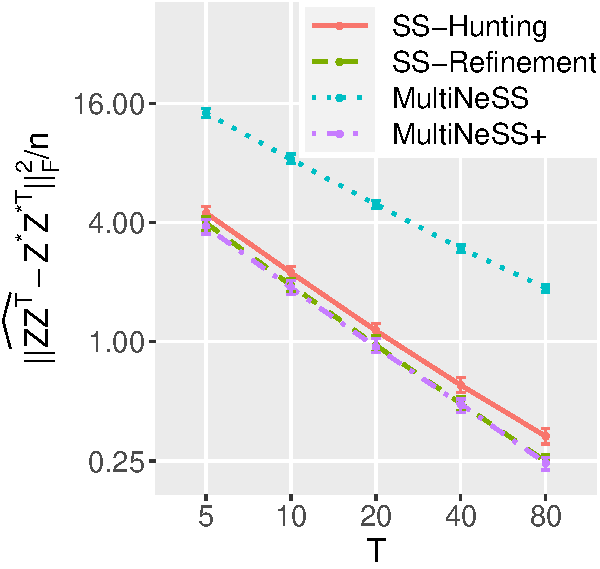
\includegraphics[width=1\linewidth]{Figures/Simu_BA.pdf}
    \caption{Bernoulli distribution}
\end{subfigure}
\begin{subfigure}{0.29\textwidth}
	\centering
	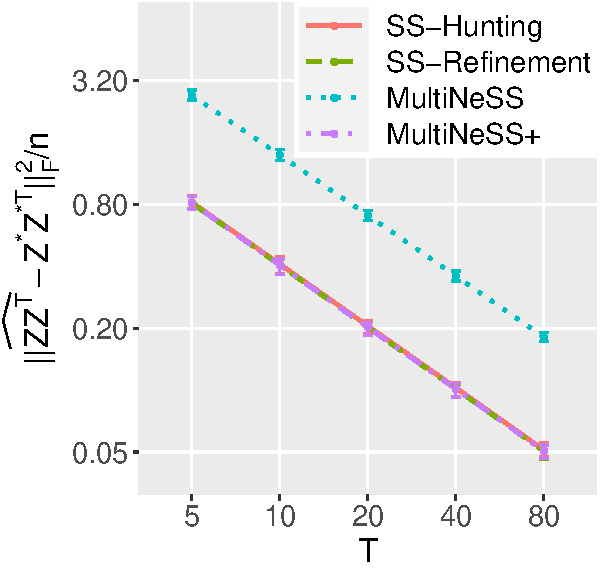
\includegraphics[width=1\linewidth]{Figures/Simu_GA.pdf}
    \caption{Gaussian distribution}
\end{subfigure}
\begin{subfigure}{0.29\textwidth}
	\centering
	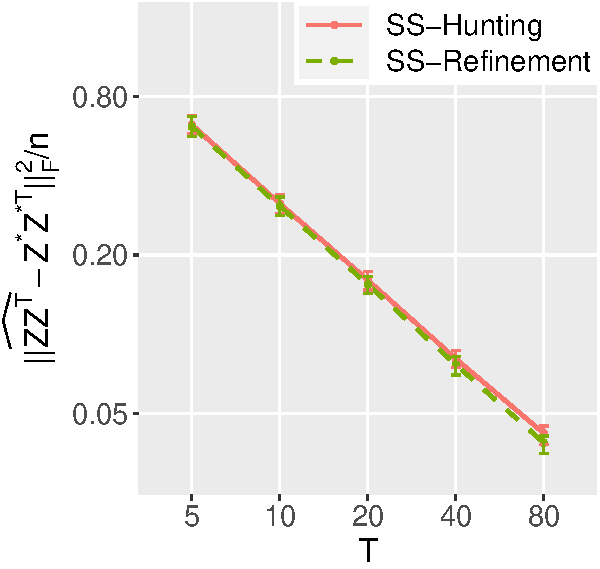
\includegraphics[width=1\linewidth]{Figures/Simu_PA.pdf}
    \caption{Poisson distribution}
\end{subfigure}
\caption{Empirical estimation errors versus $T$ under Case (A). Lines connect median estimation errors over 100 repetitions, and error bars are obtained from the 0.05 and 0.95 quantiles of those repetitions. Axes are in the log scale.}
\label{fig:simuA}
\end{figure}
\begin{figure}%[!htbp]
\centering
\begin{subfigure}{0.29\textwidth}
	\centering
	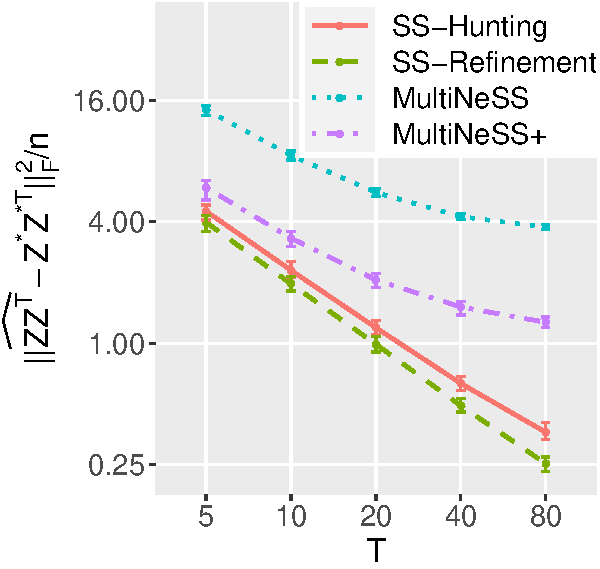
\includegraphics[width=1\linewidth]{Figures/Simu_BB.pdf}
    \caption{Bernoulli distribution}
\end{subfigure}
\begin{subfigure}{0.29\textwidth}
	\centering
	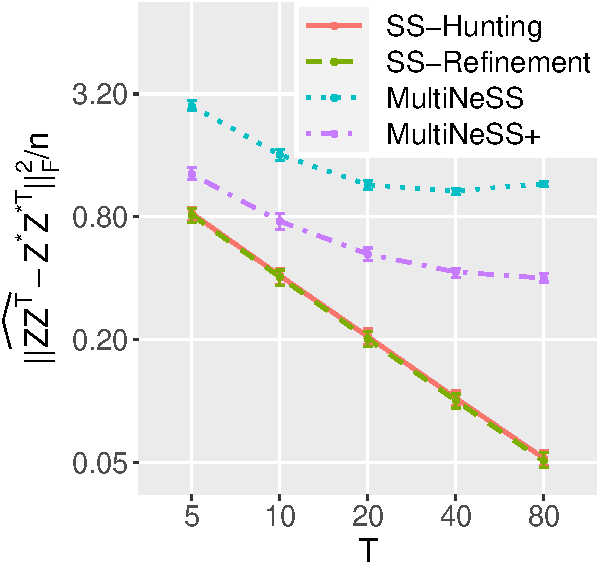
\includegraphics[width=1\linewidth]{Figures/Simu_GB.pdf}
    \caption{Gaussian distribution}
\end{subfigure}
\begin{subfigure}{0.29\textwidth}
	\centering
	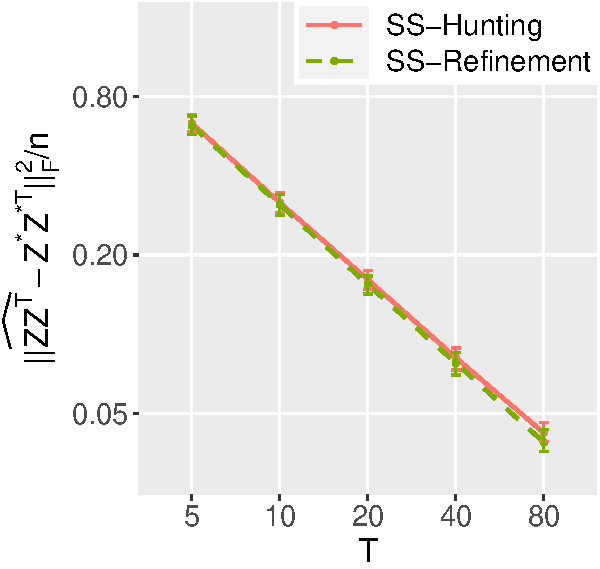
\includegraphics[width=1\linewidth]{Figures/Simu_PB.pdf}
    \caption{Poisson distribution}
\end{subfigure}
\caption{Empirical estimation errors  versus $T$ under Case (B). (Similar to Figure \ref{fig:simuA}.)}
\label{fig:simuB}
\end{figure}


Figures \ref{fig:simuA}--\ref{fig:simuC} present  empirical estimation errors of the four estimators under Cases (A)--(C), respectively. %Since the codes of MultiNeSS and MultiNeSS+ are not available under Poisson distribution, their errors are not presented under Poisson in the three figures.  
In Figure \ref{fig:simuA}, all the errors are inverse proportional to $T$, achieving the oracle error rate discussed in Section \ref{sec:challenges}. 
Among the four methods, SS-Refinement and MultiNeSS+ achieve the smallest error under different distributions. 
% Figure \ref{fig:simuB} depicts empirical estimation errors under Case (B). 
In Figure \ref{fig:simuB}, SS-Refinement achieves the smallest error across three distributions, 
while SS-Hunting performs similarly under Gaussian and Poisson distributions but not Bernoulli distribution. 
Different from Figure \ref{fig:simuA},
MultiNeSS and MultiNeSS+ no longer exhibit inverse proportional to $T$ error rates. 
Under Case (C), errors of MultiNeSS and MultiNeSS+ explode and thus are not presented in Figure \ref{fig:simuC}. 
Unlike Figures \ref{fig:simuA} and \ref{fig:simuB},  
SS-Hunting does not achieve inverse proportional to $T$ errors, whereas SS-Refinement still achieves that. 




% \begin{figure}%[!htbp]
% \centering
% \begin{subfigure}{0.29\textwidth}
% 	\centering
% 	\includegraphics[width=1\linewidth]{Figures/tmp/Simu_BA3.pdf}
%     \caption{Bernoulli distribution}
% \end{subfigure}\ 
% \begin{subfigure}{0.29\textwidth}
% 	\centering
% 	\includegraphics[width=1\linewidth]{Figures/tmp/Simu_BA3.pdf}
%     \caption{Gaussian distribution}
% \end{subfigure}\ 
% \begin{subfigure}{0.29\textwidth}
% 	\centering
% 	\includegraphics[width=1\linewidth]{Figures/tmp/Simu_BA3.pdf}
%     \caption{Poisson distribution}
% \end{subfigure}
% \caption{Empirical estimation errors versus $T$ under Case (A). Lines connect median estimation errors over 100 repetitions, and error bars are obtained from the 0.05 and 0.95 quantiles of those repetitions. Axes are in the log scale.}
% \label{fig:simuA}
% \end{figure}



\begin{figure}%[!htbp]
\centering
\begin{subfigure}{0.29\textwidth}
	\centering
	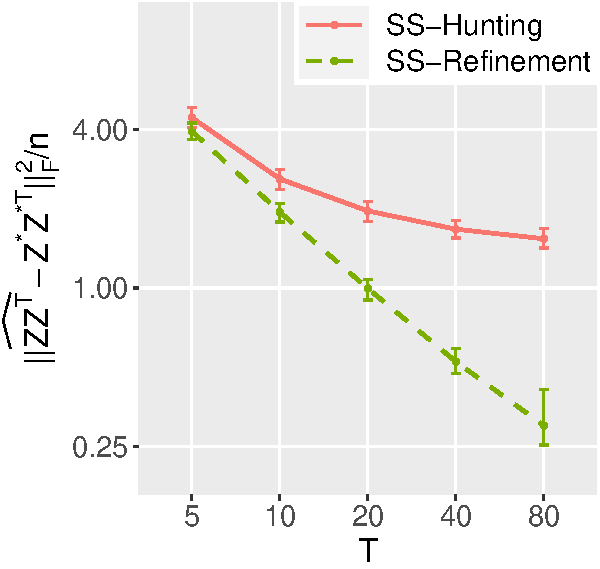
\includegraphics[width=1\linewidth]{Figures/Simu_BC.pdf}
    \caption{Bernoulli distribution}
\end{subfigure}
\begin{subfigure}{0.29\textwidth}
	\centering
	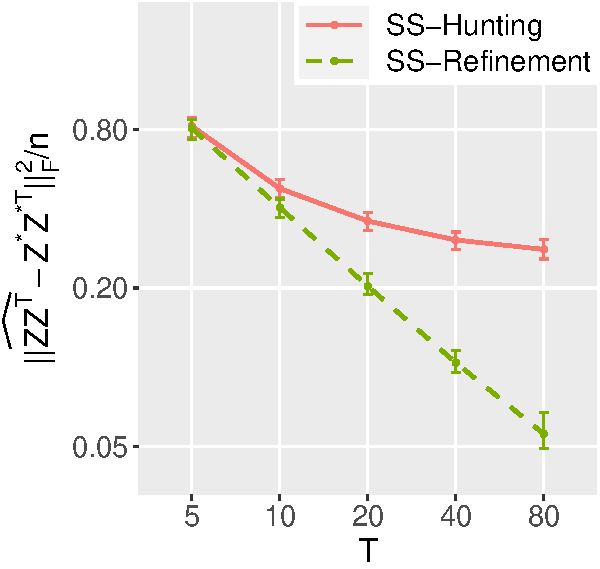
\includegraphics[width=1\linewidth]{Figures/Simu_GC.pdf}
    \caption{Gaussian distribution}
\end{subfigure}
\begin{subfigure}{0.29\textwidth}
	\centering
	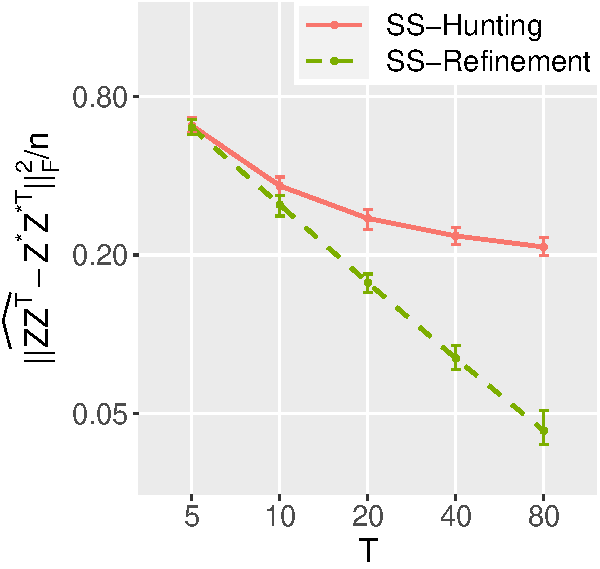
\includegraphics[width=1\linewidth]{Figures/Simu_PC.pdf}
    \caption{Poisson distribution}
\end{subfigure}
\caption{Empirical estimation errors versus $T$ under Case (C). (Similar to Figure \ref{fig:simuA}.)}
\label{fig:simuC}
\end{figure}

Intuitively, Cases (A)--(C) correspond to more and more challenging scenarios where the relationship between latent spaces become non-orthogonal and more complex. 
The non-ideal performances of MultiNeSS and MultiNeSS+ under Cases (B) and (C)
 align with Remark \ref{rmk:compare_peter} showing that our methods would require  less restriction on the latent spaces. 
 % MultiNeSS assumes nearly orthogonal conditions, while our proposed method does not have this restriction.  
% this demonstrates that in certain extreme cases, SS-Hunting can only achieve the constant rate specified in Theorem \ref{thm:initial}. 
For our two proposed estimators, 
SS-Refinement achieves the desired inverse proportional to $T$ error rate across all cases and distribution, whereas  SS-Hunting fails to achieve that in  challenging Case (C). 
% although SS-Hunting could perform  similarly to SS-Refinement in favorable scenarios, e.g., Cases (A) and (B), it 
% On the one hand, this demonstrates that in certain extreme cases, SS-Hunting can only achieve the constant rate specified in Theorem \ref{thm:initial}. 
This is consistent with our theoretical results in Theorems \ref{thm:initial} and \ref{thm:onestep} providing general error rates under weak assumptions about latent spaces. 
The results demonstrate the effectiveness of the proposed efficient estimation strategy. 
% Theorem \ref{thm:initial} is a general conclusion under weak conditions and may not represent the optimal convergence rate under more favorable circumstances. 

% \bigskip 
% Overall, all methods provide reasonable estimates, and the corresponding \blue{fitted slopes} are close to $-1$, suggesting that errors are inverse proportional to $T$. When considering the magnitude of the error, SS-Refinement and MultiNeSS+ exhibit comparable performances. However, MultiNeSS+ significantly reduces the estimation error of MultiNeSS, while SS-Refinement shows only a minor improvement compared with SS-Hunting. When comparing with the theoretical results, SS-Refinement exhibits a $1/T$ rate consistent with Theorem \ref{thm:onestep}, but SS-Hunting demonstrates a better convergence rate than predicted by Theorem \ref{thm:initial}.  It’s worth noting that the error rate of $\mathring Z$ in Theorem \ref{thm:initial} is a general conclusion under weak conditions and may not represent the optimal convergence rate under more favorable circumstances.

%\blue{discuss: Theorem \ref{thm:initial} error rates is more the joint error. We observe that the rate for $Z^{\star}$ can actually be better. } 



% The empirical estimation errors corresponding to Case B and Case C are depicted in Figure \ref{fig:simuB} and Figure \ref{fig:simuC}, respectively. Under Case B, SS-Hunting and SS-Refinement exhibit similar performance compared to that under Case A, while MultiNeSS and MultiNeSS+ no longer have a $1/T$ convergence rate. This result aligns with our discussion in Remark \ref{rmk:compare_peter} that MultiNeSS assumes nearly orthogonal conditions, while our proposed method does not have this restriction. Under Case C, MultiNeSS and MultiNeSS+ do not converge well, so they are not shown in the figure. Unlike the first two cases, SS-Refinement exhibits significant improvement compared to SS-Hunting and maintains the $1/T$ rate. On the one hand, this demonstrates that in certain extreme cases, SS-Hunting can only achieve the constant rate specified in Theorem \ref{thm:initial}. %On the other hand, this indicates that Condition \ref{cond:truevalue2} is merely a technically sufficient condition, as we discussed in Remark \ref{rm:condwextra}.








\section{Data analysis} \label{sec:data}
% To demonstrate the interpretations of , 
We analyze a multiplex-network dataset of  lawyers \citep{lazega2001collegial} to demonstrate the insights provided by examining shared and individual latent spaces. 
% the Lazega Lawyers dataset \citep{lazega2001collegial}. 
% We demonstrate the use of 
% the effectiveness of 
% the proposed method by applying it to the Lazega Lawyers dataset \citep{lazega2001collegial}. 
This dataset contains three types of connection relationships:  coworker, friendship, and advice,   between seventy-one lawyers in a Northeastern US corporate law firm. 
Within each type of network, we consider binary and undirected edges between lawyers indicating whether 
connections of each type exist between them. 
% there exist type-specific connections between them. 
% We consider undirected binary edge between two lawyers 
Since there is no ground truth of latent spaces in practice, 
we compare the estimated latent embeddings with observed node-wise features to gain insights into the results given by the proposed method and other existing methods.   

% \textcolor{gray}{The data were collected using sociometric name generators, and only the coworker network is undirected. To ensure consistency with our setup, we symmetrized the networks prior to analysis. The dataset also includes various individual attributes such as seniority, gender, office, and practice.} 

% For our proposed method, 
As network edges are binary, 
we adopt Bernoulli distribution in the model \eqref{eq:model} and estimate latent dimensions by Algorithm B.1, which gives  $\hat{k}_1 = 6$, $\hat{k}_2 = 4$, $\hat{k}_3 = 1$, and $\hat{k}=2$. 
Then we estimate  latent embedding  vectors under estimated latent dimensions by SS-Refinement.  
% In particular, we obtain  $\hat{k}_1 = 6$, $\hat{k}_2 = 4$, $\hat{k}_3 = 1$, and $\hat{k}=2$. 
As  a comparison, we also apply   MultiNeSS+ in  \cite{macdonald2022latent} and  MASE in \cite{arroyo2021inference}  with the dimension of the shared space set to be two.  

% \begin{figure}[htbp!]
% \centering
% \begin{subfigure}{0.28\textwidth}
% 	\centering
% 	\includegraphics[width=1\linewidth]{Figures/Law_Z.pdf}
%     \caption{SS-Refinement}
% \end{subfigure}
% \begin{subfigure}{0.27\textwidth}
% 	\centering
% 	\includegraphics[width=1\linewidth]{Figures/tmp/Law_Z.pdf}
%     \caption{MultiNeSS+}
% \end{subfigure}
% \begin{subfigure}{0.28\textwidth}
% 	\centering
% 	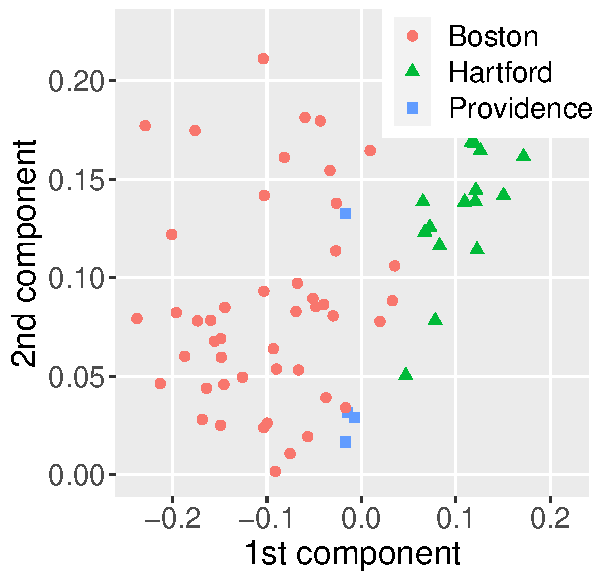
\includegraphics[width=1\linewidth]{Figures/Lawc_Z.pdf}
%     \caption{MASE}
% \end{subfigure}
% \caption{Estimated shared latent vectors $z_i$'s  using three methods.} 
% \label{fig:Z}
% \end{figure}

\begin{figure}
\centering
\begin{subfigure}{0.28\textwidth}
	\centering
	\includegraphics[width=1\linewidth]{Figures/Law_Z.pdf}
    \caption{SS-Refinement}
\end{subfigure}\quad 
\begin{subfigure}{0.28\textwidth}
	\centering
	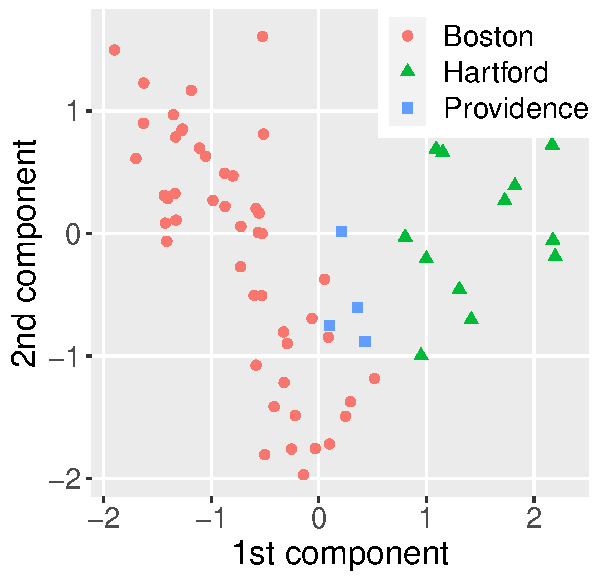
\includegraphics[width=1\linewidth]{Figures/Lawp_Z.pdf}
    \caption{MultiNeSS+}
\end{subfigure}\quad 
\begin{subfigure}{0.28\textwidth}
	\centering
	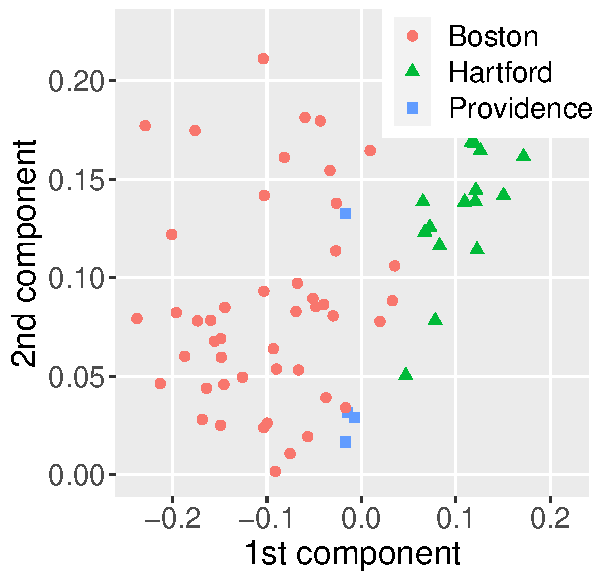
\includegraphics[width=1\linewidth]{Figures/Lawc_Z.pdf}
    \caption{MASE}
\end{subfigure}
\caption{Estimated shared latent vectors $z_i$'s  using three methods.} 
\label{fig:Z}
\end{figure}

\begin{figure}
\centering
\begin{subfigure}{0.28\textwidth}
	\centering
	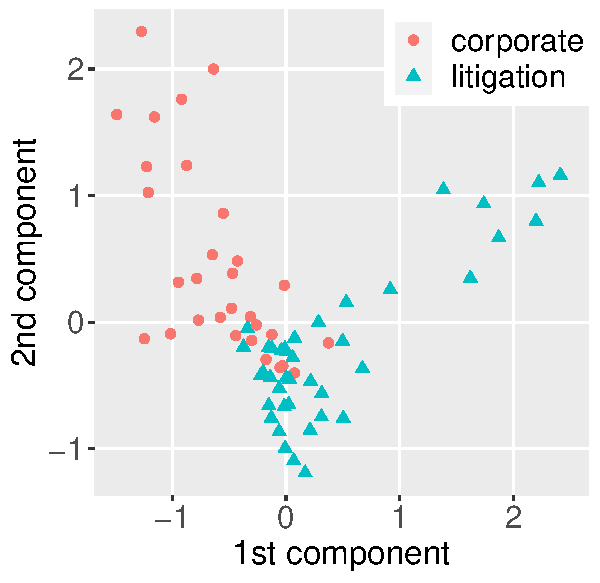
\includegraphics[width=1\linewidth]{Figures/Law_W1.pdf}
    \caption{SS-Refinement}
\end{subfigure}\quad 
\begin{subfigure}{0.28\textwidth}
	\centering
	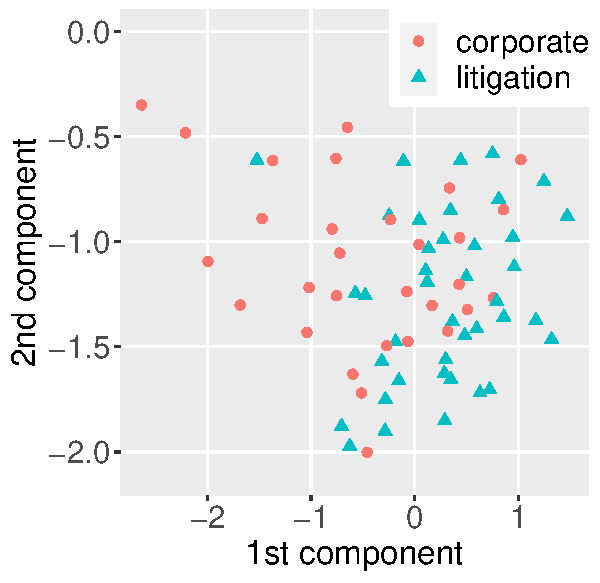
\includegraphics[width=1\linewidth]{Figures/Lawp_W1.pdf}
    \caption{MultiNeSS+}
\end{subfigure}
\caption{Estimated individual latent vectors $w_{1,i}$'s  using two methods.}
\label{fig:estW1}
\end{figure}
\begin{figure}[htbp!]
\centering
\begin{subfigure}{0.28\textwidth}
	\centering
	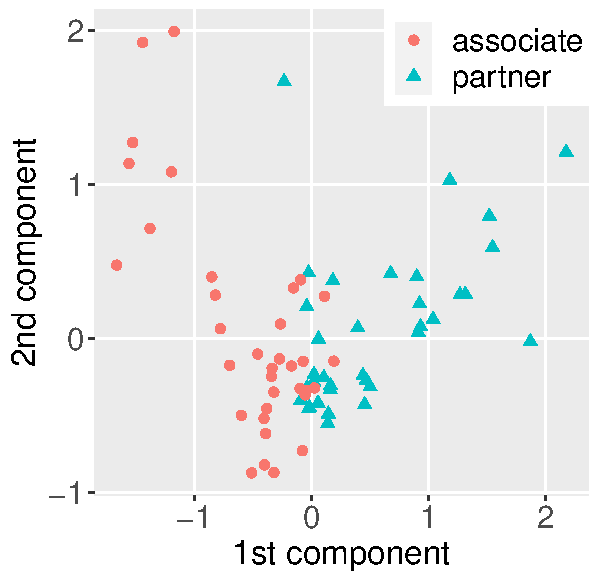
\includegraphics[width=1\linewidth]{Figures/Law_W2.pdf}
    \caption{SS-Refinement}
\end{subfigure}\quad 
\begin{subfigure}{0.28\textwidth}
	\centering
	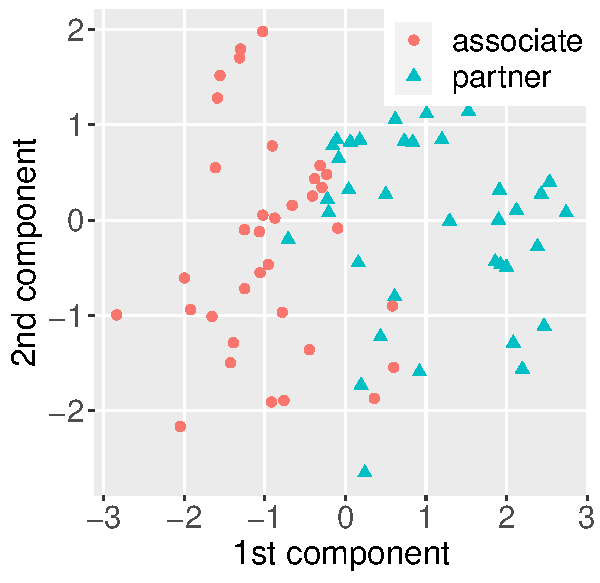
\includegraphics[width=1\linewidth]{Figures/Lawp_W2.pdf}
    \caption{MultiNeSS+}
\end{subfigure}
% \caption{Estimation of the heterogeneous latent vectors $w_{2,i}$'s  using different methods}
\caption{Estimated individual latent vectors $w_{2,i}$'s  using two methods.}
\label{fig:estW2}
\end{figure}
% Figure \ref{fig:Z} visualizes   
 % scatterplots of estimated 

 We first illustrate the 
 shared latent embeddings estimated by the three methods. 
% Under the model \eqref{eq:model}, $Z$ is i
% As the latent embeddings 
% For the  shared latent embeddings, 
Figure \ref{fig:Z} (a) and (b) present  the leading two principal component scores of the shared latent component $Z$ estimated 
% shared latent vectors projected onto the  leading two principal component directions of $Z^{\top}Z$ 
by SS-Refinement and MultiNeSS+, respectively. 
% latent vectors $Z$ estimated by SS-Refinement and MultiNeSS+ after projected onto the leading two PC directions of the shared component $ZZ^{\top}$.  
 Figure \ref{fig:Z} (c) displays latent embeddings estimated by MASE that are rotated to approximate (a) and (b) for the ease of comparison. 
% which are rotated to 
% MASE in \cite{arroyo2021inference} is applied , and 
In Figure \ref{fig:Z}, each point is colored according to the office location of the corresponding  lawyer.  
The patterns of points in Figure \ref{fig:Z} (c) slightly differ from those in (a) and (b), which could be due to the difference between models fitted.  
Nevertheless, the results of all three methods show that the shared latent embeddings are correlated with the office locations of lawyers. 
This  suggests that office locations could play a shared role in forming multiple types of connections between lawyers.  


% Figure \ref{fig:Z} (a) and (b) display similar results whereas 

% shared latent embeddings could be correlated with the office locations of lawyers. 
% the first component of $\hat{z}_i$'s 
% effectively separate people from different offices in the latent space. 
% As the visualization indicates, the first component of $\hat{z}_i$'s effectively separate people from different offices in the latent space. 
% We can see that their estimates are also effective in separating the different office populations. %\blue{In addition to the office interpretation, we also find that the remaining component of the estimated shared latent vectors correspond to the lawyers’ practice (see Figure \ref{fig:Z2} in Section \ref{sec:data supp} of the Supplementary Material). (Maybe remove this?)} 






We next compare the individual latent embeddings $W_t$'s estimated by SS-Refinement and MultiNeSS+, where we point out that MASE does not directly give  comparable estimates and thus is not included.     
% Since the model in \cite{arroyo2021inference} 
% COSIE, the underlying model of MASE, only 
% models 
% the heterogeneity of the inner product kernels across different networks, we only compare our method only with MultiNeSS+.
Figures \ref{fig:estW1} and \ref{fig:estW2}  present the estimated individual latent component  after projected to its leading two principal components for the coworker and friendship networks, respectively. 
% In Figure \ref{fig:estW1}, we present a visualization of the leading  two principal component scores of the estimated heterogeneous latent vectors for the coworker network, with
In Figure \ref{fig:estW1}, points are colored according to lawyers’ practice. 
The results show that latent vectors estimated by both two methods  demonstrate association with lawyars' practice, whereas  the separation between litigation and corporate lawyers appears to be more  obvious in estimates given by SS-Refinement. 
% Our approach provides clear separation of litigation lawyers and corporate lawyers in the first component of our estimates, while MultiNeSS+ does not accomplish effectively. 
This discrepancy might be attributed to the fact that MultiNeSS+ tends to encourage the column spaces of $Z$ and $W_t$'s to be orthogonal, which is not required in our approach and thus leads to distinct estimates in practice.   
% nearly orthogonality among the column space of $Z$ and $W_t$'s, whereas our approach requires much weaker conditions. 
% The argument is further validated by the visualization of the Gram matrix of the estimated latent vectors (see Figure \ref{fig:Gram} in Section \ref{sec:data supp} of the Supplementary Material), which shows that there exist similarities among the columns of $W_t$'s. 
% Moreover, Figure \ref{fig:estW2} visualizes the leading two principal component scores of the individual latent vectors for the friendship network, where points are colored based on the lawyers’ status. 
In  Figure \ref{fig:estW2},  points are colored based on the lawyers’ status. 
Similarly to Figure \ref{fig:estW1}, 
latent vectors estimated by both two methods exhibit correlation with a common covariate, lawyers’ status,  even though the  patterns of points are not exactly the same.  
% T indicating that both considered methods achieved clear separations between associate lawyers and partner lawyers. 



In summary, our analysis shows that investigating shared and individual latent embeddings  reveals key underlying factors driving the formation of heterogeneous multiplex networks. 
The proposed analysis paradigm could offer us a deeper understanding of multifaceted relationships and unveil  inherent structures of interlinked systems across various domains.  

% unveil fundamental structures in complex interconnected systems. 
% could provide valuable insights into the underlying factors driving the formation of heterogeneous multiplex networks. Shared and individual latent embeddings reveal multifaceted interconnected systems 



% estimated via the proposed method align well with the lawyers' attributes incorporated in the dataset. 
% \vspace{2em} 
% \textcolor{gray}{We first apply Algorithm \ref{algor:estk} to estimate the latent space dimensions that correspond to the three networks in the Lazega Lawyers dataset. According to the estimation results, the three networks share a $2$-dimensional latent space, with heterogeneous latent dimensions of $\hat{k}_1 = 6$, $\hat{k}_2 = 4$, and $\hat{k}_3 = 1$. We then fit model \eqref{eq:model} with a Bernoulli distribution and the estimated latent space dimensions through Algorithms \ref{algor:initial}--\ref{algor:refine}.  Figure \ref{fig:Z}(a) shows the estimation of the shared latent vectors $z_i$'s, with the points colored according to the lawyers' office. As the visualization indicates, the first component of $\hat{z}_i$'s effectively separate people from different offices in the latent space.} 



% \textcolor{gray}{
% To compare with other methods for multiple networks, we also perform MultiNeSS+ proposed by \cite{macdonald2022latent} and MASE proposed by \cite{arroyo2021inference}. The corresponding estimation results for $z_i$'s are presented in Figure \ref{fig:Z}(b)--(c). We can see that their estimates are also effective in separating the different office populations. In addition to the office interpretation, we also find that the remaining component of the estimated shared latent vectors correspond to the lawyers’ practice (see Figure \ref{fig:Z2} in Section \ref{sec:data supp} of the Supplementary Material). \textcolor{gray}{From the perspective of separating people with different offices and practices, our proposed method 
% is more interpretable than MultiNeSS+ and MASE.}}


% \textcolor{gray}{
% Apart from the shared latent vectors, we also focus on the heterogeneous parts of each network. Since COSIE, the underlying model of MASE, only models the heterogeneity of the inner product kernels across different networks, we compare our method only with MultiNeSS+. In Figure \ref{fig:estW1}, we present a visualization of the first two components of the estimated heterogeneous latent vectors for the coworker network, with the vectors colored according to the lawyers’ practice.  Our approach provides clear separation of litigation lawyers and corporate lawyers in the first component of our estimates, while MultiNeSS+ does not accomplish effectively. This could be attributed to the fact that MultiNeSS+ assumes the nearly orthogonality among the column space of $Z$ and $W_t$'s, whereas our approach requires much weaker conditions. The argument is further validated by the visualization of the Gram matrix of the estimated latent vectors (see Figure \ref{fig:Gram} in Section \ref{sec:data supp} of the Supplementary Material), which shows that there exist similarities among the columns of $W_t$'s. }



% \textcolor{gray}{
% Similarly, we visualize the first two components of the estimated heterogeneous latent vectors for the friendship network in Figure \ref{fig:estW2}. The estimated latent vectors are colored based on the lawyers’ status, indicating that both considered methods achieved clear separations between associate lawyers and partner lawyers. In summary, the latent vectors estimated via the proposed method align well with the lawyers' attributes incorporated in the dataset.} 




 
\section{Discussions} \label{sec:discussion}

This work establishes   
a general analysis framework for  efficient estimation of node-wise latent embeddings in multiple heterogeneous networks. 
It shows that aggregating multiplex networks can improve the efficiency of estimating shared latent spaces. 
In particular, we develop 
  a  novel two-stage approach: the first stage 
 hunts for shared latent embedding spaces,
and the second stage improves the statistical efficiency with likelihood information. 
We establish estimation error bounds for the estimators of the two stages. The final estimator has been shown to achieve the oracle rates of component for both the shared and individual components according to their dimensions.  
  The new developments would provide statistical insights into how to efficiently  aggregate heterogeneous datasets and unravel fundamental structures in complex interconnected systems. 

The new developments pave the way for a broad range of future studies. 
First, accurate estimation of latent embedding spaces plays a crucial role in  subsequent analytical tasks including, but not limited to, understanding latent confounders across multifaceted interconnected systems,  adjusting dependence of observations for causal inference  \citep{mcfowland2023estimating,nath2022identifying,hayes2022estimating}, and  prediction with or on noisy network data \citep{ma2020universal,le2022linear,lunde2023conformal}.   


Second, another interesting future research direction is to  extend the  analysis to various other network models. % with additional components to capture various connectivity patterns. 
% the  methods and theoretical techniques can be extended to  
For instance, to analyze networks exhibiting  significant degree heterogeneity, we could add network-specific and node-specific degree heterogeneity parameters in current model, similarly to   \cite{zhang2020flexible} and \cite{he2023semiparametric}. %letting 
%widely adopted in latent space models \citep{hoff2002latent,he2023semiparametric}.   
% the model \eqref{eq:model} does not  
% implicitly assumes the degree homogeneity across different nodes and time by restricting the latent vectors $y_{t,i}$ in a constant range. 
% when analyzing data with significant degree heterogeneity, a natural generalization of the model is to incorporate degree heterogeneity parameters, which is widely used in latent space models \citep{he2023semiparametric}. % \begin{align*}
%     \Theta_{t,ij} = \alpha_{it} + \alpha_{jt} + z_i^\mytrans z_j + w_{t,i}^\mytrans w_{t,j},
% \end{align*}
% In particular, we can let 
% $\Theta_{t,ij} = \alpha_{it} + \alpha_{jt} + z_i^\mytrans z_j + w_{t,i}^\mytrans w_{t,j},$
% where $\alpha_{it}$'s model the degree heterogeneity across $i \in \{1, \ldots, n\}$ and $t \in \{1, \ldots, T\}$. 
Moreover, other forms of interactions could be considered, such as using  a general kernel function beyond inner product \citep{rubin2022statistical,macdonald2022latent},
or modeling directed network edges with asymmetric latent embeddings  \citep{perry2013point,yan2019statistical}.  
% to enhance the flexibility of modeling interactions, various generalizations of modeling 
% a general kernel function beyond inner product may be adopted \citep{rubin2022statistical,macdonald2022latent},
% or one can model directed network edges with asymmetric latent embeddings  \citep{perry2013point,yan2019statistical}.  
In addition, when there are observed covariates \citep{yan2021covariate,huang2018pairwise}, it would be worthwhile to devise appropriate procedures for  covariate adjustments. %  and investigate the corresponding influences. 
The  methods and theoretical tools developed in this work provide a versatile toolbox that could be useful under  diverse scenarios of network analysis.  

Finally, our current  analysis of efficient estimation  requires the likelihood to be correctly specified.
However, in many applications, 
distributions of noisy networks  may deviate from their prespecified forms. This misspecification might alter the interpretation of latent embeddings and impede efficient estimations.   Understanding the effect of distribution misspecification would be an important future research direction. Such studies could  provide us better understanding towards underlying data structures and lead to  reliable and robust conclusions \citep{rubin2020manifold}. 
% To analyze complex data that may deviate from prespecified distributions, it would be important to 
%  understand the effect of misspecification on estimating latent embeddings. This could  provide us better understanding towards underlying data structures and draw reliable conclusions \citep{rubin2020manifold}. 

% serves as a cornerstone of 
% also be extended to this model.
% directed model: \blue{to do} 
% The paper proposes a general set of toolbox for analyzing heterogeneous networks with two steps: find shared latent spaces and then refine with high-order likelihood information. 
% The idea is flexible and can be readily generalizable. 
% For instance, in addition to hunting shared spaces in $Y_t$, 
% one may also hunt for shared space in $W_t$'s again and conduct sequential analysis.{ \color{gray} For example,
% use space hunting on the $W_t$'s; or,
% a penalty term like $\sum_{t_1,t_2} \lambda_{t_1,t_2} \operatorname{dist}^2(W_{t_1}, W_{t_2}) $, with adaptive lasso type of tuning on $\lambda_{t_1,t_2}  $ }


% combine with heterogeneous kernels COSIE model and kernels in  \cite{macdonald2022latent}
% discuss that if \begin{itemize}
%     \item $\hat{k}=0$
%     \item $\hat{k}_t=0$ 
% \end{itemize}
% our procedure could also provide inforamtion on whether there exsit shared factors


% Several additional components that could be integrated into our model to capture a wider range of effects are outlined below. Firstly, apart from capturing interaction effects through latent position inner products, the model could be enriched by incorporating marginal effects.
% % captured by degree heterogeneity parameters across nodes and layers. 
% For example, in the lawyer network data, beyond the primary interaction effects governed by variables such as the lawyer’s office, practice, and position, certain lawyers might be more active in the coworker network, while some others may be more engaged in the friendship network. Such individual-level effects could be modeled using degree heterogeneity parameters across nodes and layers. A natural modification to the model specifications \eqref{eq:modeltheta} and \eqref{eq:model2} is expressed as 
% \begin{align*}
%    g(\mathbb{E}[A_{t,ij}|\pmb\alpha,Z,W] ) =  \Theta_{t,ij} = \alpha_{it} + \alpha_{jt} + z_i^\mytrans z_j + w_{t,i}^\mytrans w_{t,j},
% \end{align*}
% where $\alpha_{it}$'s model the degree heterogeneity across nodes $i \in \{1, \ldots, n\}$ and layers $t \in \{1, \ldots, T\}$. We point out that our current estimation algorithms and theoretical analysis can also be extended to this model. Secondly, to accommodate directed network data, where the in-edges and out-edges of nodes may exhibit distinct behaviors, we are interested in developing a model for asymmetric adjacency. A possible parametrization based on  \eqref{eq:modeltheta} and \eqref{eq:model2} is given by
% \begin{align*}
%    g(\mathbb{E}[A_{t,ij}|Z,W] ) =  \Theta_{t,ij} = z_i^{(out) \mytrans} z_j^{(in)} + w_{t,i}^{(out) \mytrans} w_{t,j}^{(in)} ,
% \end{align*}
% where $A_{t,ij}$  denotes the directional edge from node $i$ to node $j$ in layer $t$, whose connectivity is determined by the inner product of the ``out latent vectors'' of $i$ and the ``in latent vectors'' of $j$. From a modeling perspective, this model invites further exploration into the similarities and differences between the learned in and out latent structures. From a theoretical point of view, the identifiability and information matrix eigenstructure of the asymmetric model are different from symmetric models, potentially necessitating novel technical advances.
% Thirdly, akin to the single network model studied in \cite{hoff2003random,hoff2005bilinear} and the network event history data studied in \cite{perry2013point}, integrating covariates into our model represents a worthwhile pursuit.  A potential adjusted form of the model specification \eqref{eq:modeltheta} is
% \begin{align*}
%    g(\mathbb{E}[A_{t,ij}|Z,W] ) =  \Theta_{t,ij} = z_i^\mytrans z_j + w_{t,i}^\mytrans w_{t,j} +  X_{t,ij}^\top \pmb\gamma ,
% \end{align*}
% where $X_{t,ij} $ denotes the time-varying covariate for the $i$-$j$ edge, and $\pmb\gamma$ is the regression coefficient vector. Covariate adjustment via regression can help unveiling more complex network structures and enhance downstream tasks such as link prediction \citep{ma2020universal,huang2018pairwise}.





 

% \appendix

% \begin{center}
%     \huge \textbf{Appendix} 
% \end{center}



\vspace{-1em}
\section*{Supplementary Material}
Due to space limitation, additional details, including individual estimation in Section \ref{sec:estimateyt}, estimating latent dimensions, and proofs are deferred to the Supplementary Material.

% \small
% \bibliographystyle{ims}
\bibliographystyle{apalike}
\begin{spacing}{1.5}
    \bibliography{Citation.bib}
\end{spacing}

\end{document}
